%%%%%
%%
%% Sample document ``thesis.tex''
%%
%% Version: v0.2
%% Authors: Jean Martina, Rok Strnisa, Matej Urbas
%% Date: 30/07/2008
%%
%% Copyright (c) 2008-2011, Rok Strniša, Jean Martina, Matej Urbas
%% License: Simplified BSD License
%% License file: ./License
%% Original License URL: http://www.freebsd.org/copyright/freebsd-license.html
%%%%%

% Available documentclass options:
%
%   <all `report` document class options, e.g.: `a5paper`>
%   withindex   - enables the index. New index entries can be added through `\index{my entry}`
%   glossary    - enables the glossary.
%   techreport  - typesets the thesis in the technical report format.
%   firstyr     - formats the document as a first-year report.
%   times       - uses the `Times` font.
%   backrefs    - add back references in the Bibliography section
%
% For more info see `README.md`
\documentclass[withindex, glossary]{cam-thesis}
\usepackage[table]{xcolor}% http://ctan.org/pkg/xcolor

% Citations using numbers
\usepackage[numbers]{natbib}
% \usepackage[dvipsnames]{xcolor}
\usepackage{graphicx,wrapfig,lipsum}

\usepackage[export]{adjustbox}
% \usepackage[square,sort,comma,numbers]{natbib}

% Include other packages here, before hyperref.
\usepackage{graphicx}
\usepackage{booktabs}
%\usepackage{algorithmic}
%\usepackage{algorithm}
\usepackage{textcomp}
\usepackage{mathtools,xparse}

\usepackage[linesnumbered,ruled,vlined]{algorithm2e}
\usepackage{algpseudocode}

\usepackage{stfloats}
\usepackage{url}
\usepackage{verbatim}
\usepackage{xcolor}
\usepackage{amsmath}
\usepackage{pdfpages}
\usepackage{glossaries}

\usepackage{listings}

\DeclarePairedDelimiter\abs{\lvert}{\rvert}%
\DeclarePairedDelimiter\norm{\lVert}{\rVert}%

\usepackage{subcaption}
\usepackage{float}
\usepackage{stfloats}

\usepackage{lscape}

\usepackage{hyperref}
\hypersetup{
    colorlinks=true,
    linkcolor=blue,
    filecolor=magenta,      
    urlcolor=cyan,
    pdftitle={Overleaf Example},
    pdfpagemode=FullScreen,
    }

\renewcommand{\algorithmiccomment}[1]{$\triangleright$\textit{#1}}


\usepackage{lipsum} % Only used to generate random text.
% \usepackage{natbib}
% \usepackage[pagebackref,breaklinks,colorlinks]{hyperref}

% The "axessiblity" package can be found at: https://ctan.org/pkg/axessibility?lang=en
\usepackage[accsupp]{axessibility}  % Improves PDF readability for those with disabilities.

\usepackage{bm}


\newcommand{\TODO}[1]{\textbf{\color{cyan}[TODO: #1]}}
%%%%%%%%%%%%%%%%%%%%%%%%%%%%%%%%%%%%%%%%%%%%%%%%%%%%%%%%%%%%%%%%%%%%%%%%%%%%%%%%
%% Thesis meta-information
%%

%% The title of the thesis:
\title{Data-efficient Neural\\
Appearance Manipulations}

%% The full name of the author (e.g.: James Smith):
\author{Fazilet Gokbudak}

%% College affiliation:
\college{Queens' College}

%% College shield [optional]:
% \collegeshield{CollegeShields/Christs}
% \collegeshield{CollegeShields/Churchill}
% \collegeshield{CollegeShields/Clare}
% \collegeshield{CollegeShields/ClareHall}
% \collegeshield{CollegeShields/CorpusChristi}
% \collegeshield{CollegeShields/Darwin}
% \collegeshield{CollegeShields/Downing}
% \collegeshield{CollegeShields/Emmanuel}
% \collegeshield{CollegeShields/Fitzwilliam}
% \collegeshield{CollegeShields/Girton}
% \collegeshield{CollegeShields/GonCaius}
% \collegeshield{CollegeShields/Homerton}
% \collegeshield{CollegeShields/HughesHall}
% \collegeshield{CollegeShields/Jesus}
% \collegeshield{CollegeShields/Kings}
% \collegeshield{CollegeShields/LucyCavendish}
% \collegeshield{CollegeShields/Magdalene}
% \collegeshield{CollegeShields/MurrayEdwards}
% \collegeshield{CollegeShields/Newnham}
% \collegeshield{CollegeShields/Pembroke}
% \collegeshield{CollegeShields/Peterhouse}
\collegeshield{CollegeShields/Queens}
% \collegeshield{CollegeShields/Robinson}
% \collegeshield{CollegeShields/Selwyn}
% \collegeshield{CollegeShields/SidneySussex}
% \collegeshield{CollegeShields/StCatharines}
% \collegeshield{CollegeShields/StEdmunds}
% \collegeshield{CollegeShields/StJohns}
% \collegeshield{CollegeShields/Trinity}
% \collegeshield{CollegeShields/TrinityHall}
% \collegeshield{CollegeShields/Wolfson}
% \collegeshield{CollegeShields/FitzwilliamRed}

%% Submission date [optional]:
% \submissiondate{November, 2042}

%% You can redefine the submission notice [optional]:
% \submissionnotice{A badass thesis submitted on time for the Degree of PhD}

%% Declaration date:
\date{My Month, My Year}

%% PDF meta-info:
\subjectline{Computer Science}
\keywords{one two three}



%%%%%%%%%%%%%%%%%%%%%%%%%%%%%%%%%%%%%%%%%%%%%%%%%%%%%%%%%%%%%%%%%%%%%%%%%%%%%%%%
%% Abstract:
%%
\abstract{%
  Recent works on appearance manipulation leverage deep learning techniques to achieve high-quality edits. However, such methods often rely on large amounts of data, making them undesirable in data-scarce regimes. In this thesis, I explore neural appearance manipulation techniques specifically designed for data-limited environments. More specifically, I aim to constrain the solution space of editing tasks with limited data through priors that are either imposed or learned through training.
  
    I first begin with exploring implicit appearance manipulations that work directly in the image domain without explicit information about the appearance, such as reflectance or illumination. Focusing on a low-level detail retouching task, I propose a machine learning framework that learns the style from only a single image pair. This is achieved by leveraging the priors observed in how photographers manually edit photos. Continuing within the image domain, I later explore a more complex appearance manipulation task, transient attribute transfer, utilising a diffusion model in a zero-shot setting.

    Despite their effectiveness and efficiency, working in the image domain presents challenges regarding controllability over appearance. For instance, editing each material individually within an image is complicated, requiring an additional segmentation algorithm to separate the materials \cite{}. Furthermore, patch-space information is intertwined with illumination, which is difficult to estimate \cite{}. Therefore, as an alternative to implicit editing, I explore explicit appearance modelling that aim for sparse reconstruction with real-world applications in physically-based rendering systems. I propose a neural material representation model that excels in generalising to new materials, editing existing appearances, and compressing them. This model can be integrated into either a rendering or a capture system. While rendering offers finer control capabilities in scene editing, capture systems serve as the engine for such rendering processes.

    In summary, my thesis focuses on neural network-based appearance editing suitable for data-scarce problem spaces. Here, I explore scene manipulation in two distinct aspects: 1) image-based implicit editing, encompassing both low-level and high-level editing, and 2) explicit appearance modelling with a neural Bidirectional Reflectance Distribution Function (BRDF) estimation. These approaches have the potential to significantly advance research in efficient and realistic appearance editing, offering valuable contributions to the research community working on similar subjects.

}



%%%%%%%%%%%%%%%%%%%%%%%%%%%%%%%%%%%%%%%%%%%%%%%%%%%%%%%%%%%%%%%%%%%%%%%%%%%%%%%%
%% Acknowledgements:
%%
\acknowledgements{%

}



%%%%%%%%%%%%%%%%%%%%%%%%%%%%%%%%%%%%%%%%%%%%%%%%%%%%%%%%%%%%%%%%%%%%%%%%%%%%%%%%
%% Glossary [optional]:
\makeglossaries

\newglossaryentry{MLP}{
    name=MLP,
    description={Multilayer Perceptron}
}

\newglossaryentry{LLF}{
    name=LLF,
    description={Local Laplacian Filter}
}

\newglossaryentry{BRDF}{
    name=BRDF,
    description={Bidirectional Reflectance Distribution Function}
}
\newglossaryentry{HVS}{
    name=HVS,
    description={Human Visual System}
}
\newglossaryentry{SGD}{
    name=SGD,
    description={Stochastic Gradient Descent}
}

\newglossaryentry{DDIM}{
    name=DDIM,
    description={Denoising Diffusion Implicit Models}
}

%%%%%%%%%%%%%%%%%%%%%%%%%%%%%%%%%%%%%%%%%%%%%%%%%%%%%%%%%%%%%%%%%%%%%%%%%%%%%%%%
%% Contents:
%%
\begin{document}

%%%%%%%%%%%%%%%%%%%%%%%%%%%%%%%%%%%%%%%%%%%%%%%%%%%%%%%%%%%%%%%%%%%%%%%%%%%%%%%%
%% Title page, abstract, declaration etc.:
%% -    the title page (is automatically omitted in the technical report mode).
\frontmatter{}



%%%%%%%%%%%%%%%%%%%%%%%%%%%%%%%%%%%%%%%%%%%%%%%%%%%%%%%%%%%%%%%%%%%%%%%%%%%%%%%%
%% Thesis body:
%%


\chapter{Introduction}



%\marginpar[Margin note.]{Margin par.}



\section{Overview} 

The appearance of a 3D scene comprises the visual features that are shaped by the interaction of light with materials, textures, and geometry, defining how we perceive objects in terms of colour, shading, and surface detail. Many factors, including lighting conditions, material properties, and environmental effects, affect appearance. Lighting, the type, location, intensity and colour of light sources, define how objects are illuminated, generating shadows, highlights, and overall contrast. Materials describe the optical properties of objects, such as base colour, transparency, reflectivity, and surface roughness. Textures are 2D images or procedural patterns applied to 3D surfaces, providing detailed surface information, such as colour, bumpiness, or imperfections. The 3D models' geometric detail and surface topology affect how light interacts with objects. Atmospheric conditions such as fog, reflections, and global illumination contribute to the overall appearance by simulating real-world environmental factors. The position and properties of the virtual camera, including focal length and field of view, influence the composition, perspective, and the visual hierarchy of objects in the scene. Overall, appearance is a result of the interplay between light, material properties, surface detail, and environmental factors, all of which contribute to the perceptual qualities and realism of the rendered image.

Appearance manipulations refer to the edits of the aforementioned visual features, ranging from retouching intricate details to transforming entire scenes. Appearance manipulation techniques are instrumental in the success of multiple fields with real-world applications. In filmmaking, it helps create realistic special effects or offers subtle changes to lighting, costumes, and even an actor’s appearance during post-production. In social media and advertising, it allows users to benefit from filters, face-tuning, and other aesthetic tools. In augmented and virtual reality (AR/VR) platforms, it enables embodying human avatars that improve immersive realism, including changing hairstyles, outfits or body types. In fashion and e-commerce, users can trustfully shop clothes or accessories online through virtual try-ons. Even the fact that Richard Linklater had filmed the movie "Boyhood" (2014) over 12 years to capture the natural aging of the actors shows the necessity and importance of precise appearance manipulation techniques across disciplines. Therefore, this thesis is dedicated to tackle the challenging task of appearance manipulations with learning-based techniques with the hope that the proposed approaches can alleviate some of the difficulties that editors come across, such as accuracy, the scarcity of data, etc. This thesis investigates the three distinct perspectives of appearance (fine details, transient attributes, reflectance representations) and presents data-efficient machine learning approaches for accurate and visually-pleasing manipulations.

Earlier approaches to manipulate scene appearance involve traditional image processing/computer graphics techniques and extensive manual editing in dedicated software platforms, such as Photoshop, Lightroom, Blender or Unreal Engine. These traditional editing approaches require significant time and skill due to the complexity and scale of the transformations involved. On the other hand, recent advancements in machine learning techniques starting with convolutional neural networks and reaching the current state of generative models have paved the way for precise and natural-looking appearance transfers that maintain the photorealism of the rendered scene. For instance, we can now instruct programs to edit images in only a few seconds thanks to the developing field of generative AI. Furthermore, the deep learning models have allowed us to represent naturally continuous signals as continuous neural functions, which were before bounded to the discrete representations. Consequently, machine learning techniques have revolutionised appearance manipulation by generating high-quality, realistic renderings from data inputs. However, the main bottleneck in these approaches is the scarcity of the training data that can drastically reduce the performance of the ML models. For instance, the number of pixels that belong to details is significantly lower than those belonging to low-frequency components, or obtaining the real "summer" - "winter" image pair can require us to wait for months. Furthermore, capturing the real-world reflectance measurements of even relatively simple materials takes hours in a professional capture setup. For these reasons, this thesis specifically focuses on generalisable approaches that can manipulate appearance with data efficiency.


Appearance manipulation has become an indispensable tool in modern visual culture, driving innovation in entertainment, healthcare, and beyond. AI's involvement enhances the accuracy, scalability, and creativity of appearance modifications, pushing the boundaries of what is visually possible and enabling more seamless and engaging user experiences across industries.


\subsection{One-shot Detail Retouching}

\begin{figure}[ht]
  \centering
  % \fbox{\rule{0pt}{2in} \rule{0.9\linewidth}{0pt}}

    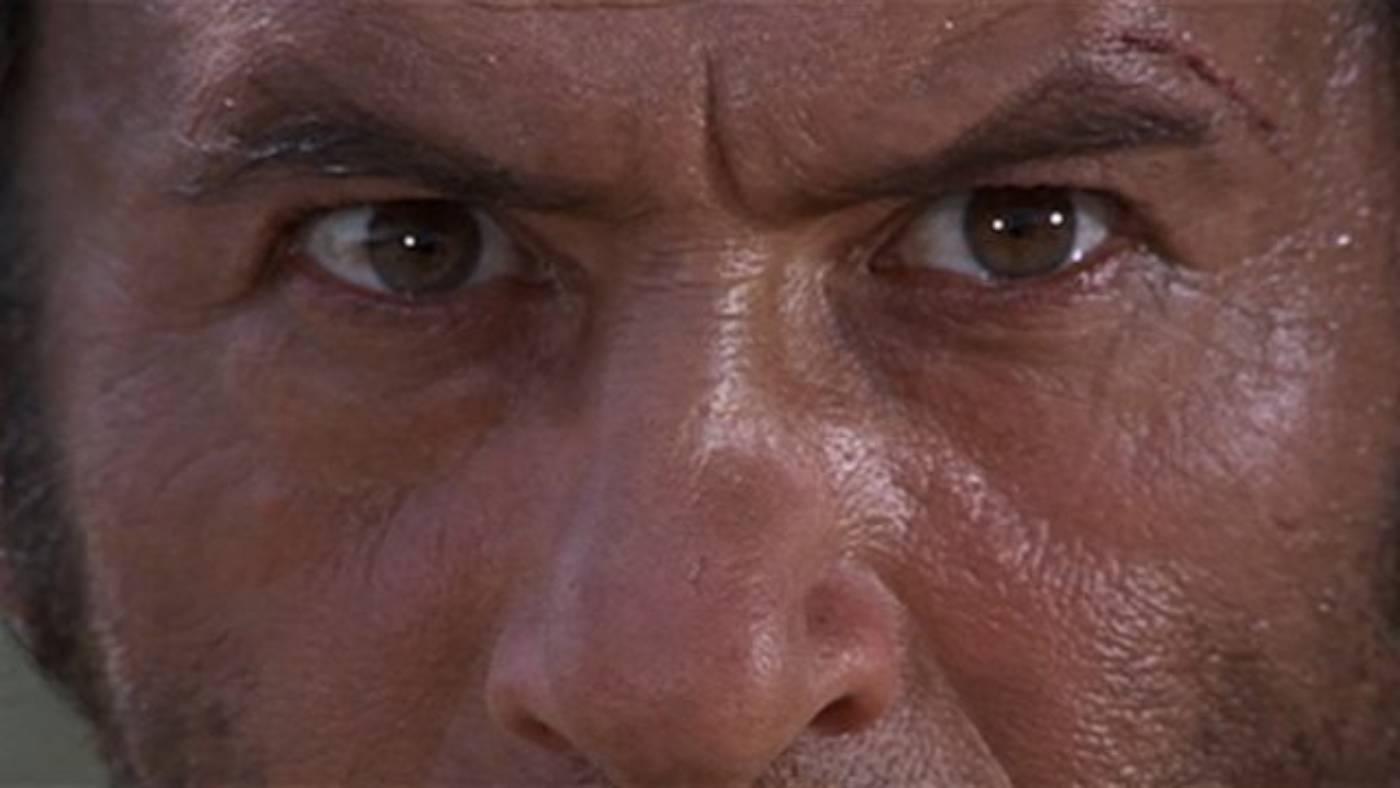
\includegraphics[width=\linewidth]{Images/A scene from ‘The Good, the Bad and the Ugly’ (1966). Image courtesy- Produzioni Europee Associati .jpg}

   \caption{A pixel, a picture element, is the smallest unit of a rendered image. Displaying an image with fewer pixels causes losses in details as one pixel starts covering a larger area in the 3D scene.}
   \label{fig:colour-approximate}
\end{figure}


\begin{wrapfigure}{r}{5cm}
  \centering
  % \fbox{\rule{0pt}{2in} \rule{0.9\linewidth}{0pt}}
   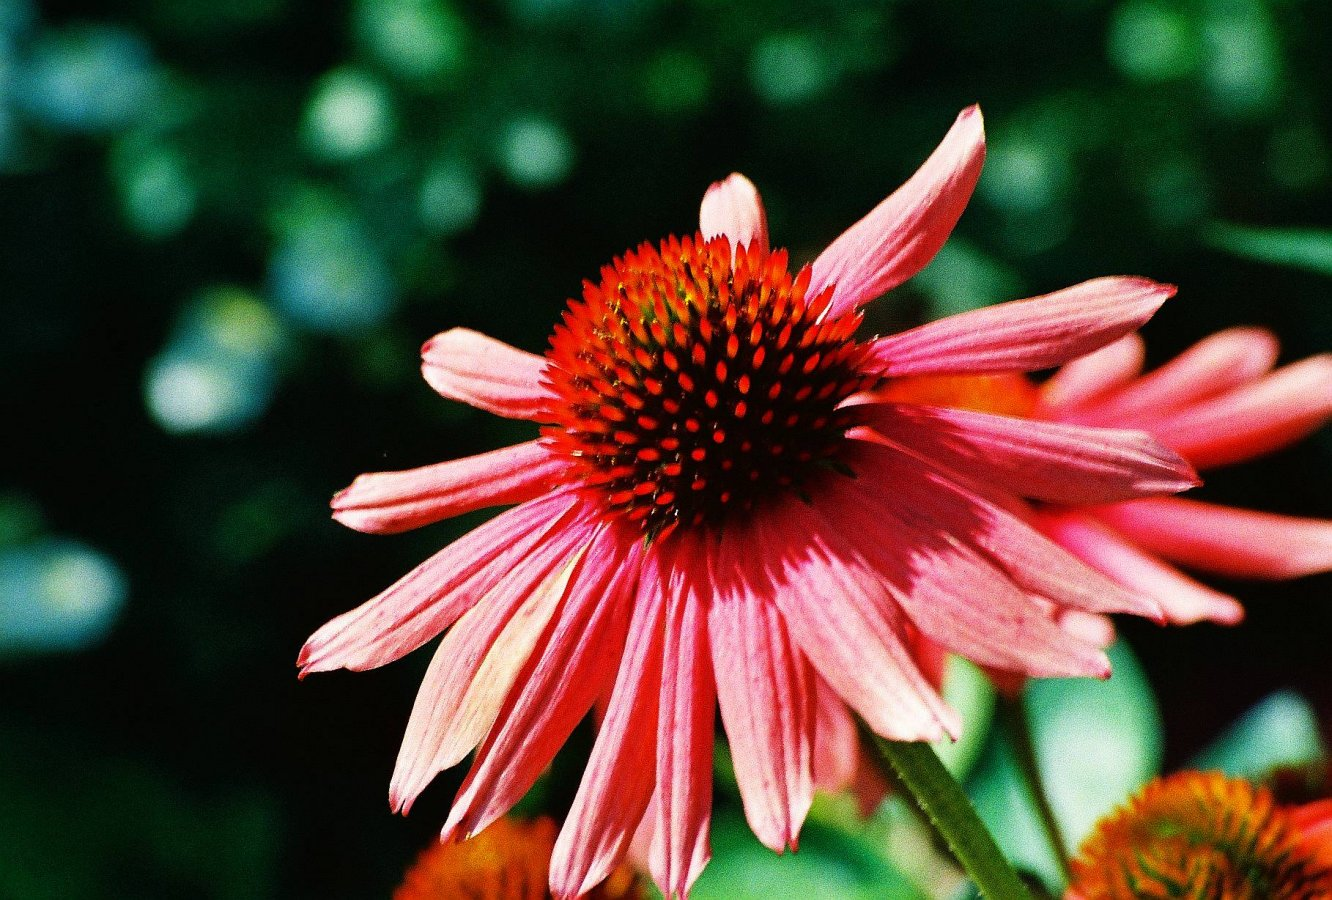
\includegraphics[width=\linewidth]{Images/byRickJones .jpg}
   
   \caption{Graph representation of a linear equation. Figure from [Issac, 2018].}
   \label{fig:neuron}
\end{wrapfigure}

\subsection{Transient Attribute Transfer}
\begin{figure}[ht]
  \centering
  % \fbox{\rule{0pt}{2in} \rule{0.9\linewidth}{0pt}}

    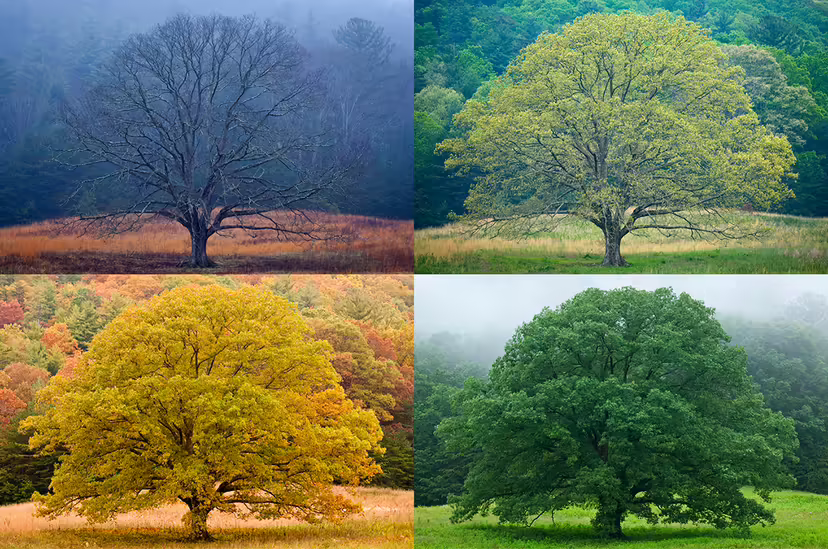
\includegraphics[width=\linewidth]{Images/seasonchanges.png}

   \caption{A pixel, a picture element, is the smallest unit of a rendered image. Displaying an image with fewer pixels causes losses in details as one pixel starts covering a larger area in the 3D scene. Image from [Michael Melford/Getty Images]}
   \label{fig:colour-approximate}
\end{figure}

\subsection{Generalisable Neural BRDF Representation}

\begin{figure}[ht]
  \centering
  % \fbox{\rule{0pt}{2in} \rule{0.9\linewidth}{0pt}}

    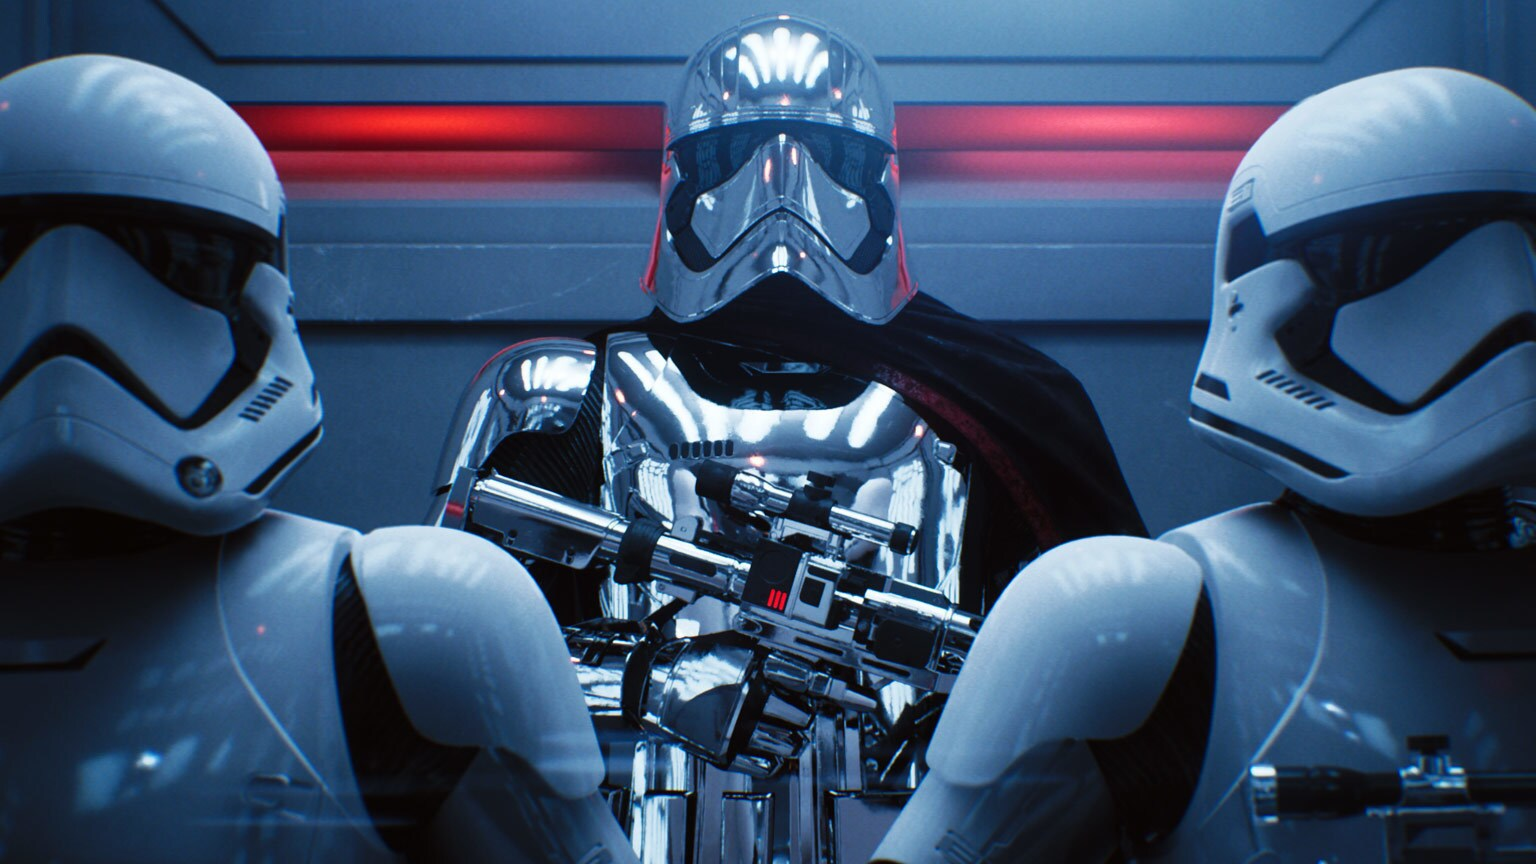
\includegraphics[width=\linewidth]{Images/StarWars-RayTracing.jpeg}

   \caption{Photorealistic rendering can be achieved through extensive ray tracing for which reflectance should be accurately measured and represented.}
   \label{fig:colour-approximate}
\end{figure}



\section{Contributions}
\section{Publications}

The following works are produced throughout my doctoral studies and contributed to main chapters of this dissertation:

\begin{itemize}

\item \textbf{Fazilet Gokbudak}, Alejandro Sztrajman, Chenliang Zhou,  Fangcheng Zhong, Rafal Mantiuk, and Cengiz Oztireli. Hypernetworks for Generalizable BRDF Representation. \textit{ECCV 2024}

\item \textbf{Fazilet Gokbudak} and Cengiz Oztireli. Text-guided Transient Attribute Transfer. \textit{Under review}.

\item \textbf{Fazilet Gokbudak} and Cengiz Oztireli. One-shot Detail Retouching with Patch Space Neural Transformation Blending. \textit{In Proceedings of the 20th ACM SIGGRAPH European Conference on Visual Media Production (CVMP '23)}, 2023. Association for Computing Machinery, New York, NY, USA, Article 2, 1–10. https://doi.org/10.1145/3626495.3626499

\end{itemize}

The following works did not directly contribute to this dissertation; however, they helped me build skills and knowledge for the success of the main contributions:

\begin{itemize}

\item Madeleine Darbyshire, Shaun Coutts, Eleanor Hammond, \textbf{Fazilet Gokbudak}, Cengiz Oztireli, Petra Bosilj, Junfeng Gao, Elizabeth Sklar, and Simon Parsons. Multispectral Fine-Grained Classification of Blackgrass in Wheat and Barley Crops. \textit{Under Review}, 2024.

\item Chenliang Zhou, Alejandro Sztrajman, Rainer Gilles, and Fangcheng Zhong, \textbf{Fazilet Gokbudak}, Zhilin Guo, Weihao Xia, Rafal Mantiuk, and Cengiz Oztireli. Physically Based Neural Bidirectional Reflectance Distribution Function. \textit{Under Review}, 2024.

\end{itemize}

Furthermore, the work I completed during my internship at Amazon 
\chapter{Background}

% \section{Rendering an Image of a 3D Scene}
\section{Rendering}

This section gives an overview of rendering an image of a 3D scene to connect the image-level appearance with a broader concept of appearance representations in computer graphics.  It starts with the display of images on a screen and elaborates on 3D scene components that are taken into account for photorealistic rendering, mainly focusing on appearance. 

\subsection{Displaying an image}
An image is displayed on a computer screen or, in general, a display system after the stored data is processed in a computer. Here, the computer and the display system operate with discrete data, known as bits and pixels. Considering real-world objects as continuous structures, the object shapes need to be broken down into discrete surfaces (pixels) for their display as an image. This operation is known as discretisation. 

\begin{figure}[ht]
  \centering
  % \fbox{\rule{0pt}{2in} \rule{0.9\linewidth}{0pt}}

    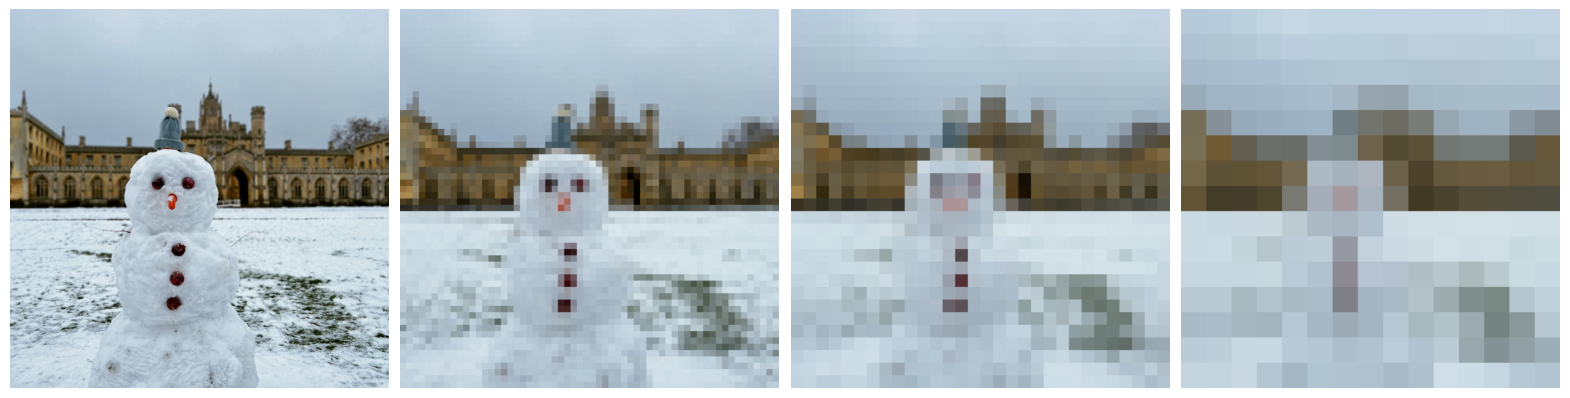
\includegraphics[width=\linewidth]{Images/pixelate_image_snowman.png}

   \caption{A pixel, or picture element, is the smallest unit of a rendered image. Displaying an image with fewer pixels results in a loss of detail, as each pixel begins to cover a larger area in the 3D scene.}
   \label{fig:colour-approximate}
\end{figure}

Let's consider the display of a sphere on a computer screen. We apply a grid on the sphere to represent pixels. Some pixels have a constant colour of the object, while some are blank. On the other hand, some pixels include different shades of the object colour or some are half-overlapped with the sphere. The question here is how to fill the pixels with mixed colours. 

In a simple case where we only have a single colour with a blank background, we can subdivide this pixel into sub-pixels and count the number of pixels that belong to the object and the background. Later, the colour of the corresponding pixel can be approximated by taking the weighted average between the background and object colour. For instance, Figure \ref{fig:display-grid} shows the display of a sphere with grids symbolising pixels. The sub-pixels on the right can be counted to compute the colour of the corresponding large pixel. The generalised implementation of this approach can be seen in Figure \ref{fig:colour-approximate}, where I computed the mean value with a sliding window of different sizes (50, 100 and 200 in order, for image size of 3024 x 4032).

\begin{figure}
  \centering
  % \fbox{\rule{0pt}{2in} \rule{0.9\linewidth}{0pt}}
   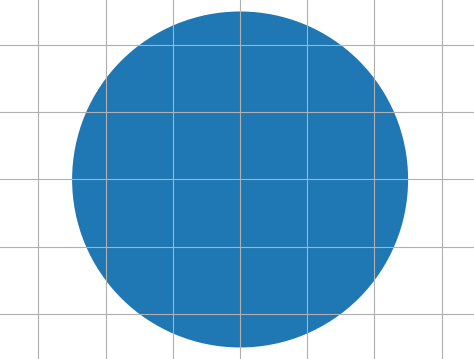
\includegraphics[width=0.48\linewidth]{Images/grid_circle.png}
    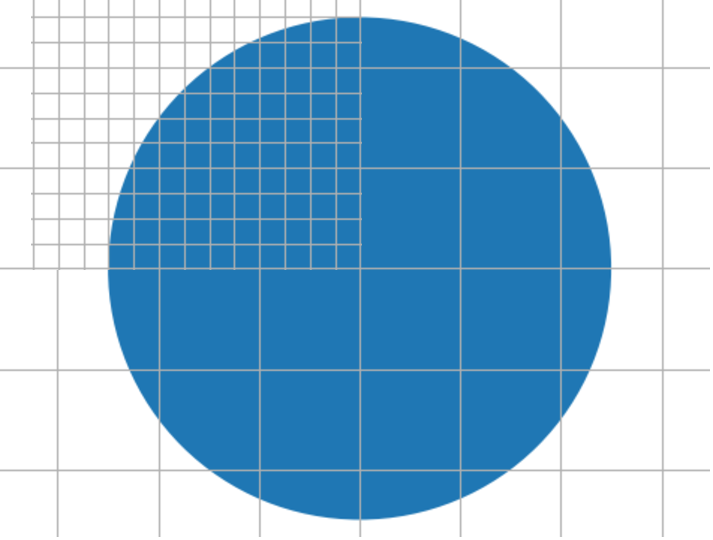
\includegraphics[width=0.48\linewidth]{Images/merged_grid_circle2-crop.pdf}

   \caption{To compute the colour of a pixel with variations, it is common practice to divide the pixel into sub-pixels and take the weighted average of each sub-pixel.}
   \label{fig:display-grid}
\end{figure}


\begin{wrapfigure}{l}{6cm}
\includegraphics[width=\linewidth]{Images/colourspace.png}
\caption{Comparison of different colour gamuts. Image from [Schewe and Fraser, 2007].}\label{fig:colour-gamut}
    
\end{wrapfigure} 

Another approach would be to increase the resolution of an image, defined by the number of pixels per image. Nonetheless, this improvement is constrained by the screen’s resolution. As we endeavour to simulate the real world, the discretisation process remains a part of this virtual representation. Furthermore, it is not merely the surface of objects that requires discretisation; the colour of each pixel must also be pieced into bits for digital storage. In other words, the number of colours we can display is restricted by the number of bits used for colour encoding. 

In the developing stages of computing, the brightness of each pixel was represented by a single bit: a value of one for white and zero for black. These days, one of the most commonly used colour spaces, standard RGB space (\gls{sRGB}), encodes each colour with 8 bits, requiring $8 * 3 = 24$ bits per pixel. Figure \ref{fig:colour-gamut} compares different colour spaces for the range of available colours in their space, known as colour gamut. Here, the question about pixel colour computation changes to how we can display a colour that is unavailable in a colour space. This problem is known as colour quantisation. The solution would be again approximating the desired colour with the closest matching colour available in the space/palette.

% \begin{figure}
%   \centering
% \caption{Comparison of different colour gamuts \cite{schewe2007colour}}\label{fig:colour-gamut}
%     \includegraphics[width=0.44\linewidth]{Images/colourspace.png}
% \end{figure} 
% %-----------------


The issue with colour quantisation is that few colour samples might not accurately represent the continuous colour spectrum, causing discrete steps, bands, between the colour samples (Figure \ref{fig:colour-band}). Luckily, the current image formats allow 24 (\gls{sRGB}) / 32 (\gls{RGBA}) bits to encode colours, displaying more than 16 million distinct colours, reducing the colour banding effect significantly. Nevertheless, the representation of continuous signals in the virtual environment remains limited due to the discretisation of the data with bits for storage in a computer.

Another problem to consider is aliasing, which occurs when the sampling frequency for discretisation is lower than twice the continuous signal bandwidth (Nyquist Theorem). The range of frequencies you can capture in a scene depends on the image resolution or pixel size. For instance, if an object is too far from the image plane, its projection can become smaller than the pixel size, for which we end up seeing the object as a dot.



\begin{figure}
  \centering
    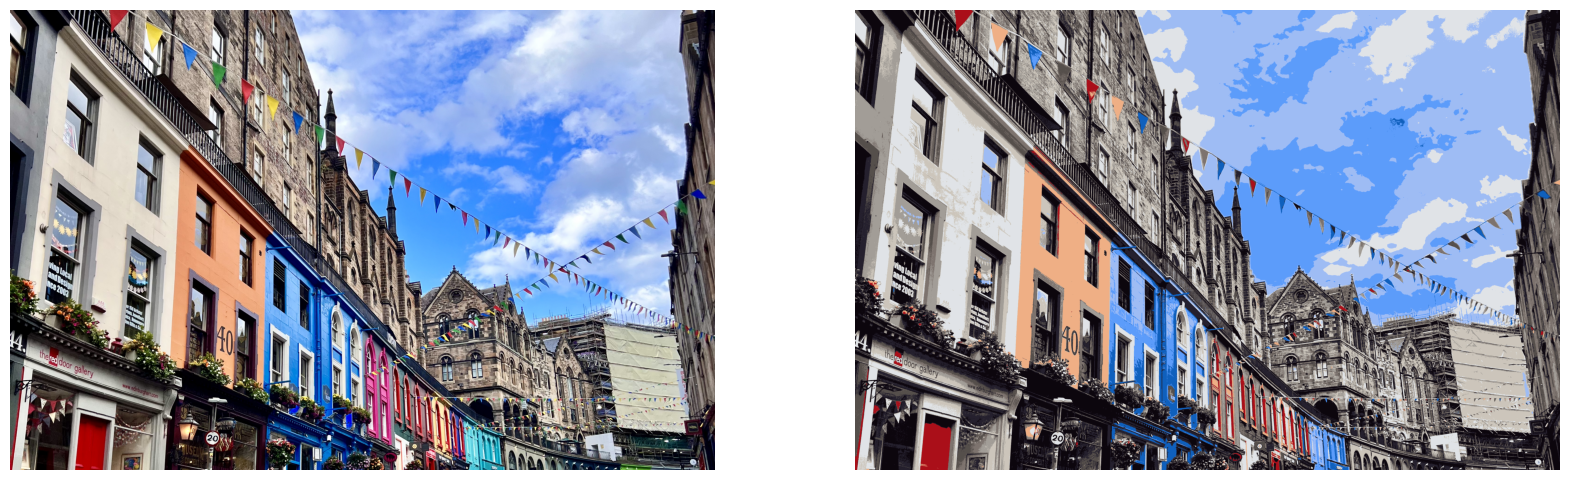
\includegraphics[width=\linewidth]{Images/colour_quantization.png}

    \caption{When a colour is represented with too few bits, the transition between colours appears as discrete steps, known as colour banding (right).}\label{fig:colour-band}
\end{figure} 


Note that the pixel-based display discussed above is called raster graphics or raster display. It lays the image onto a two-dimensional array of pixels with a grid of $x$ and $y$ coordinates on a display space. Here, zoom-in does not bring any additional details due to limitations of the image and screen resolution. On the other hand, vector graphics stores the shape of objects with mathematical expressions instead of pixel values, offering flexibility with the resolution as the shape of the objects is computed based on the desired resolution.

\subsection{3D scene components}

A 3D scene consists of objects of different sizes, shapes, and appearances. To render an image of a scene, we first need a viewpoint represented by a camera. This mimics the case in the human visual system (\gls{HVS}), where we look at a scene from a certain point, and the image of the scene appears in our retina. Without any light, all scene components appear dark. Therefore, light is a crucial aspect of the scene description. Another aspect is geometry, which defines the shape of the objects. Geometry, camera and light are three essential components of a 3D scene. While rendering a scene in a 3D software platform, such as Blender or Maya, a scene file contains all this information along with material/texture details. The light-material interaction defines the appearance, which this thesis focuses on. Before delving into the details of what appearance means in computer graphics, I will briefly review geometry as it builds up a baseline for appearance representations.

\begin{figure}[ht]
  \centering
  % \fbox{\rule{0pt}{2in} \rule{0.9\linewidth}{0pt}}
   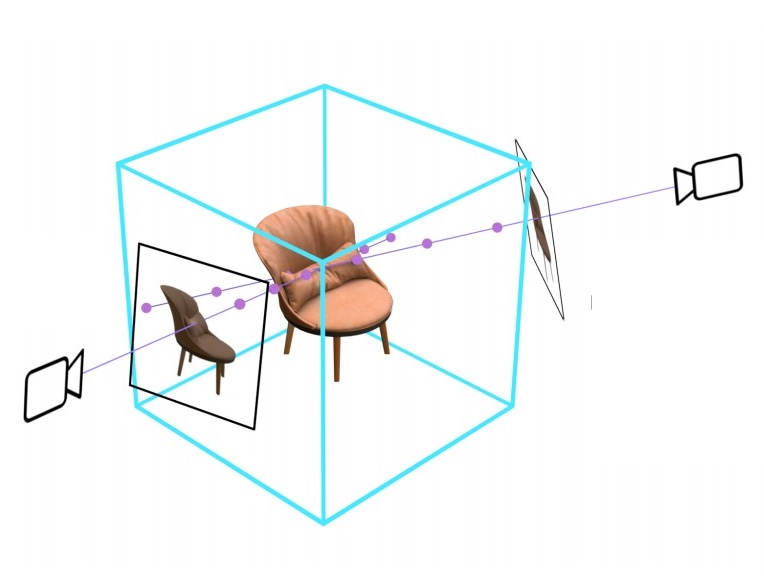
\includegraphics[width=\linewidth]{Images/scene_with_camera.jpg}
   \caption{Rendering an image of a 3D scene requires lighting, viewpoint (camera) and geometry. Image from [Boss et al., 2021].}
   \label{fig:teaser}
\end{figure}


\paragraph{Geometry.} In the real world, what differentiates the state of the objects is the density of the matter the objects consist of. For instance, clouds are made up of loosely connected molecules with large holes in between. Wood and metal are densely composed with little space between the molecules. On the other hand, computer graphics assumes that objects are either solid or not, keeping things simple since the external shape of an object is what matters at the end. 


In general, the shape of an object is represented with 3D points in computers' memory, with $x$, $y$, $z$ axes defined in the Cartesian coordinate system. The surface (a polygon) can be constructed by connecting multiple points on the same plane (co-planar). The simplest polygon we can create is a triangle. Triangles are widely used because of their simplicity and efficiency, which led to the development of multiple efficient algorithms to compute the intersection of a triangle with a line. In case surfaces are defined by many points, it is common to divide them into multiple triangles, known as triangulation. Although the real-world objects are not naturally polygonal, this simplification helps efficient rendering and digital representation.

\begin{figure}
  \centering
  % \fbox{\rule{0pt}{2in} \rule{0.9\linewidth}{0pt}}
   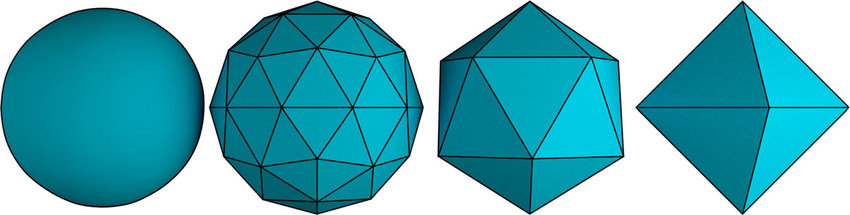
\includegraphics[width=\linewidth]{Images/Triangulation-of-surfaces-Any-curved-surface-in-this-case-a-sphere-can-be-approximated.png}
   \caption{Triangulation of surfaces is a commonly used method in computer graphics to define the shape of objects. It enables the creation of complex shapes by breaking them down into smaller triangles. Increasing the number of triangles enhances the resolution of the shape, leading to smoother and more detailed surface representations. Image from [Broeren et al., 2019].}
   \label{fig:triangulation}
\end{figure}

One might wonder how triangulation handles the reconstruction of smooth surfaces. It is indeed not an optimal solution. However, considering a smooth curve, we can approximate it by taking a few points (samples) on the curve and connecting them with straight lines (segments). To enhance the resolution, we can take more samples, that is, reduce the size of the segments. By applying this to smooth surfaces, we can increase the number of triangles (Figure \ref{fig:triangulation}) that will eventually increase the rendering time. Converting a smooth surface to triangular mesh is known as tessellation.

Returning to the early discussion on discretisation, computer graphics only approximates the shape of real-world continuous objects with discrete data. Since the ultimate goal is to display these shapes on a screen that also operates with discrete data, one well-known approach to conceal the triangular look of a surface is to keep the size of the triangles smaller than the pixel size. This approach has been used widely in professional rendering programs, such as Pixar's RenderMan, and has recently taken its place in real-time applications.

Ray tracing algorithms, which HyperBRDF is built on, do not necessarily need a polygonal representation of objects. Ray tracing computes the intersection point of a ray (a straight line) with the object surface, which can be found either with a geometric or an algebraic solution. The algebraic solution becomes feasible when the surfaces are defined by mathematical equations, known as implicit/algebraic surfaces. A ray equation, essentially a line equation, and the mathematical equation for the surface of an object give us a system of linear equations for which a solution exists if the ray and the object intersect.

Although geometry can be defined using various methods, such as meshes, NURBS, subdivision surfaces, implicit surfaces, etc., this section focuses solely on polygonal mesh representation. Triangles are the most common rendering primitives used in ray tracing and modern GPUs. As supporting a single primitive type is preferred for simplicity and efficiency, most 3D platforms convert geometry to triangular meshes before rendering.
 
\subsection{Photorealistic rendering}
There are various approaches to rendering an image of a scene, but regardless of the chosen method, the expectation is to produce the same image output. In photorealistic rendering, which is often the most desired approach, the goal is for the rendered image to appear as it would to the human eye, much like a photograph. Achieving such photorealism requires an understanding of two key aspects of our visual system: 1) the geometric construction of shapes in relation to other objects, and 2) the physical laws governing appearance. Specifically, photorealistic rendering focuses on simulating the behaviour of light as it propagates and interacts with matter.

\paragraph{Perspective projection and visibility.}

The human visual system is inherently an optical system that converges light rays reflected from objects to a focal point. Following the geometry, our eyes perceive objects that are further away smaller than the closer objects of the same size. In other words, objects get smaller in the rendered image in our retina as they move away from our eyes, known as the foreshortening effect. The lens systems in cameras already replicate this effect, and photorealistic rendering also aims to achieve the foreshortening effect along with simulating the physics laws for appearance.  

To achieve foreshortening effect, imagine we have a canvas or an image plane between the eye and the object. By tracing the lines from the eye to the corners of the objects, we can find the location of the projected corners (points) on the image plane (perspective projection). We can then draw the objects' edges on the image plane to complete the look. However, this look is unlikely to be photorealistic as we haven't figured what edges are visible from the viewpoint. For instance, if it were an opaque cube, then the back sides would remain hidden behind the front sides. Therefore, rendering involves computations for both the visibility problem and the perspective projection. 

\begin{figure}[ht]
  \centering
  % \fbox{\rule{0pt}{2in} \rule{0.9\linewidth}{0pt}}
   \includegraphics[width=\linewidth]{Images/perspective_projection.png}
   \caption{Perspective projection mimics the foreshortening effect our visual system creates while observing a scene. The image plane/canvas includes the 2D projections of the visible objects within the view frustum.}
   \label{fig:perspective_projection}
\end{figure}


We can project a 3D scene onto a flat surface in different ways. For instance, in artistic drawing, perspective projection can include multiple focal points (Figure \ref{fig:artistic_drawing}). However, computer graphics generally assumes one-point perspective as it mimics our visual system as well as cameras. In this approach, the line of sight, the line from the eye perpendicular to the canvas, passes through the centre of the canvas. The view frustum is the region of the scene projected onto the canvas. The lines passing through the corners of the canvas forms the frustum base (Figure \ref{fig:perspective_projection}). Here, we can change the size of the canvas, which results in the change of the frustum size and, consequently, the visible region of the scene. This resembles the techniques in photography where changing the focal length of the camera lenses adjusts the field of view.

\begin{figure}[ht]
  \centering
  % \fbox{\rule{0pt}{2in} \rule{0.9\linewidth}{0pt}}
   \includegraphics[width=0.48\linewidth, height=4.5cm]{Images/single_point_perspective.png}
    \includegraphics[width=0.48\linewidth, height=4.5cm]{Images/two_points_perspective.png}

   \caption{Single-point vs two-point perspective. Computer graphics mimics our visual system, focusing on single-point projection. However, multi-point perspective is widely explored in artistic drawing.}
   \label{fig:artistic_drawing}
\end{figure}


% \paragraph{Visibility problem}
The visibility problem occurs when some parts of the scene are not visible from a known viewpoint. For instance, if we only project the corners of an object and draw the edges, then some corners that shouldn't be visible from the known viewpoint will be included in the rendered image. Furthermore, some objects will be occluded by others. Computer graphics tackles the visibility problem in two ways: rasterisation and ray tracing. I will not go into the details of these algorithms as this is beyond the focus of this thesis.

% In this section, I will mostly focus on ray tracing as HyperBRDF is designed for such renderers.photorealistic rendering aims to project or flatten a 3D scene onto an image plane that lies between the scene and the camera position or the viewpoint. Mimicking our visual system, we first apply perspective projection via similarity formula in geometry and then decide which points are visible from the viewpoint. Some will be indeed occluded by other objects or the front sides. 

\paragraph{Appearance.}
Perspective projection and visibility only project the size and shape of the scene realistically without any consideration for appearance, such as the colour, texture, and brightness. We can only perceive an object if the light bounces off its surface. Therefore, appearance involves light-matter interactions, where the light travels in a ray form in space and gets absorbed or reflected when it interacts with the surface of an object. Different light sources, such as the sun or light bulbs, can emit light. After the light bounces off a surface, it continues its journey until it either reaches our eyes, where it is converted to electrical signals or another surface where the interaction steps repeat.

\begin{wrapfigure}{l}{4.8cm}
  \centering
  % \fbox{\rule{0pt}{2in} \rule{0.9\linewidth}{0pt}}
   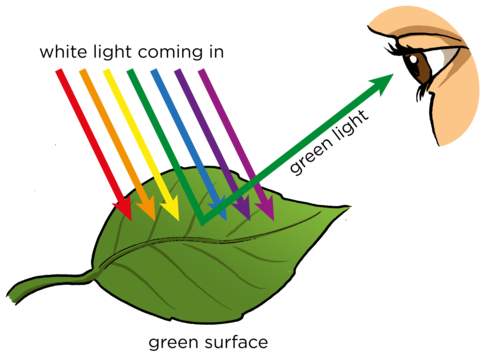
\includegraphics[width=\linewidth]{Images/object-colour.png}
   \caption{The reflected light from the surface of an object defines its colour. Image from \href{http://www.mstworkbooks.co.za/natural-sciences/gr8/images/gr8ec04-gd-0027.png}{website link}.}
   \label{fig:object-colour}
\end{wrapfigure}

The colour of an object is defined by the mixture of the reflected light colours (Figure \ref{fig:object-colour}). The light colour is a continuous spectrum with the visible light lying between 380 to 700 nanometers in wavelength. For instance, a leaf reflects green light while absorbing the remaining visible spectrum. Another example would be a black object that absorbs all visible lights or a white object that reflects them all.

At the object level, reflection can be considered a mirror-like look, where the light turns around the normal to the surface at the point of contact. The outgoing direction becomes the reflected version of the incoming one. Microscopic level interactions are more complex with light bouncing off in random directions, known as scattering. Computing the photon-atom interactions is indeed impractical. Therefore, computer graphics researchers have developed mathematical models to simulate the light-matter interactions at the microscopic level. I will discuss them later in this chapter. Section \ref{hyperbrdf-RW} will also compare HyperBRDF with such mathematical formulas. Here, I will overview some of the well-known shading and lighting effects:

\textbf{\textit{Reflection}} occurs when light interacts with mirror-like objects that change the direction of light in the reverse direction with the same angle reflected around the point of contact. The incoming light, also known as the incident light, turns around the normal and leaves the surface in the reflected/outgoing direction (Figure \ref{fig:microfacet} - right). Metals, such as silver and aluminium are considered materials with high reflectivity. The surface of the water or glass also creates reflection, but their reflectivity is considerably lower.

\textbf{\textit{Specular reflection}} appears when the surface is not perfectly smooth, and its roughness causes lights to bounce off in different directions. Consider a rough surface at the microscopic level having many microfacets looking in slightly different directions. The complex nature of the material surface then reflects the lights at a microfacet level, each microfacet acting as a mirror (Figure \ref{fig:microfacet}). The overall outgoing light becomes the combination of each of these reflections, known as specular or glossy reflection. Most often, these microfacets are not visible to our eyes akin to smooth surface appearance. The deviation of lights from the mirror direction depends on how rough the surface is, that is, how varied the facet orientations are with respect to a smooth surface. More microfacets with higher variance in orientations will lead to greater divergence from the mirror angle, enlarging the glossy region of the surface. Here, roughness and glossiness are used antonymous to describe the specularity of a material. This kind of reflection often leads to blurred or deformed images, as shown in Figure \ref{fig:water_reflection}. 


\begin{figure}
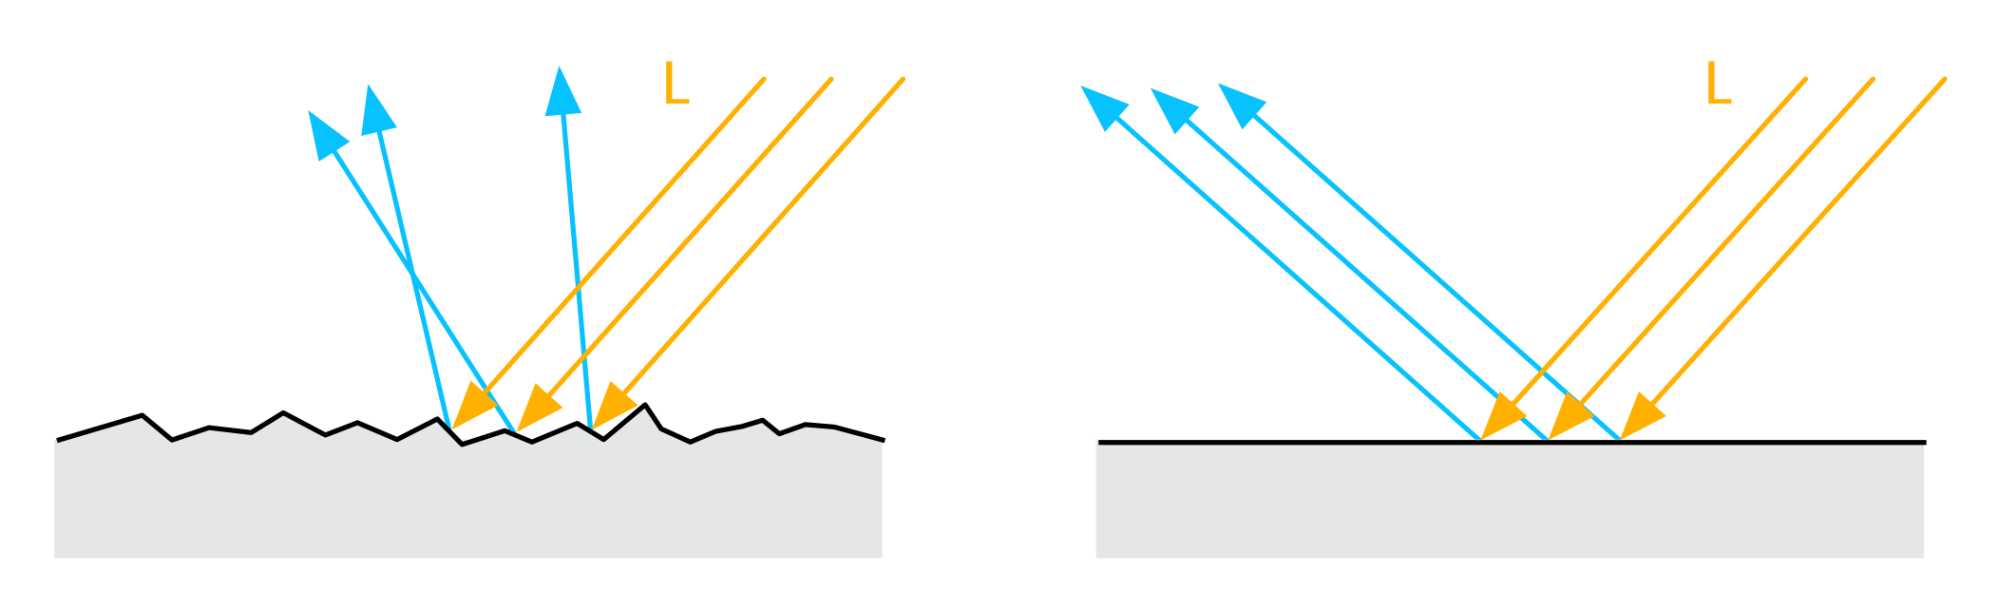
\includegraphics[width=\linewidth]{Images/diagram_microfacet.png}
\caption{Reflection on a surface with microfacets vs smooth surface. Image from [Guy and Agopian, 2024]}\label{fig:microfacet}
\end{figure} 

\begin{wrapfigure}{r}{5.4cm}
\includegraphics[width=\linewidth]{Images/rough_river_surface_reflection.png}
\caption{The ripples on the water's surface cause a blurred image of the bridge, acting as a rough surface.}\label{fig:water_reflection}
\end{wrapfigure}  

% \begin{figure}
%   \centering
%   % \fbox{\rule{0pt}{2in} \rule{0.9\linewidth}{0pt}}
%    \includegraphics[width=0.5\linewidth]{Images/rough_river_surface_reflection.png}
%    \caption{The ripples on the surface of the water causes a blurred image of the bridge, acting like a rough surface.}
%    \label{fig:water_reflection}
% \end{figure}


\textbf{\textit{Diffuse reflection}} is the reflection that we observe when the incident lights are so scattered that they reflect in random directions, equally spread. Diffuse surfaces are either extremely rough or composed of tiny structures where the light gets trapped, reflected and refracted multiple times before leaving the surface (Figure \ref{fig:diffuse-scattering}). The outgoing direction becomes independent from the incident direction due to the large number of internal reflections underneath the surface. This randomness results in the object appearing equally bright in all viewing directions. 

\begin{figure}[ht]
  \centering
  % \fbox{\rule{0pt}{2in} \rule{0.9\linewidth}{0pt}}
   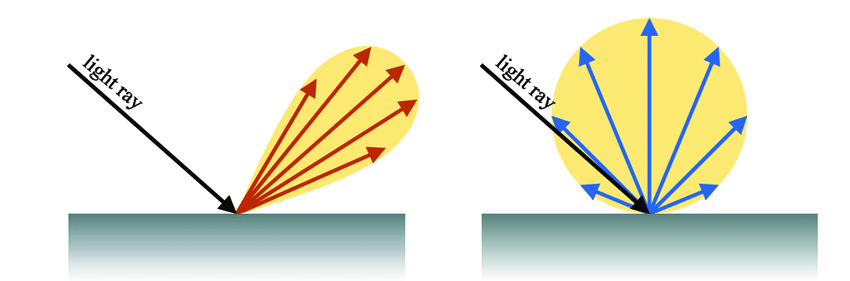
\includegraphics[width=\linewidth]{Images/Differences-between-the-specular-and-diffuse-reflections-specuclar-reflections-occur-on.png}
   \caption{Specular vs diffuse reflection. Diffuse surfaces cause rays to scatter randomly, brightening the object equally in all viewing directions. Specular reflection is, on the other hand, view-dependent, reflected rays concentrated around the mirror reflection. Image from [Park and Baek, 2021].}
   \label{fig:specularvsdiffuse}
\end{figure}

\begin{wrapfigure}{l}{6.5cm}
  \centering
  % \fbox{\rule{0pt}{2in} \rule{0.9\linewidth}{0pt}}
   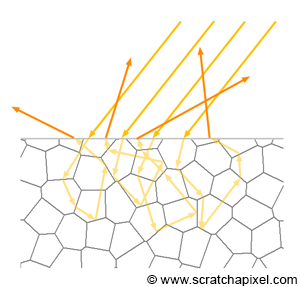
\includegraphics[width=0.5\linewidth]{Images/shad-diffuse1.png}
   \caption{Diffuse surfaces often have complex internal structures that cause the light to be reflected multiple times underneath the surface.}
   \label{fig:diffuse-scattering}
\end{wrapfigure}

Diffuse surfaces, also known as Lambertian or matte surfaces, differ from specular ones in that diffuse materials are often formed of multiple internal pieces that trap the light, causing the light's outgoing direction to become independent from the viewpoint. Specular ones, on the other hand, are modelled with microfacets that reflect the light rays around the mirror angle, remaining correlated with the incoming direction. As diffuse reflections are view-independent, the brightness of a diffuse surface remains consistent across all viewing angles (Figure \ref{fig:specularvsdiffuse}). This distinction can be observed when looking at real-world materials, observing how their brightness changes when we move around, changing our viewpoint.


Some other lighting and shading effects include transparency, subsurface scattering, indirect lighting and shadows. When light contacts a transparent object, such as glass or water, it bends and passes through the surface in a different direction, which can be computed using Snell's Law. Subsurface scattering, also known as translucency, occurs when light travels within the object, leaving the object at a different point and direction. Wax, marble or thin layers of skin are considered as translucent objects. Indirect lighting is the result of the light being reflected from other surfaces, illuminating the object without any direct light from the light source. Lastly, shadows are dark regions due to light being blocked by an object. 

The appearance of a scene depends on how light interacts with an object and the path light travels through. All the aforementioned effects contribute to appearance. Some effects, such as reflection, specularity, diffuse, transparency and subsurface scattering, relate to material properties. They affect shading, the appearance of an object. Other effects (shadows and indirect lighting) depend on the light's journey (light transport), that is, how much light the object gets after the light interacts with multiple surfaces. 

Shading is concerned with the interaction of light with the material. Light transport tracks the light's path throughout its journey while it bounces off surfaces. It takes into account the obstructions, changes of reflections, etc. In the real world, the two are not differentiated as they determine the appearance together. However, computer graphics keep these two distinct for efficient and practical computations. It is worth mentioning that simulating light-matter interactions is more challenging than tracking the light path. The latter is more straightforward, while the former requires simplifications for the material representations.



\paragraph{Ray tracing - Light transport simulation.}

Light starts its journey from a light source and travels in a straight line, bouncing off surfaces. Following this path to simulate the light is known as forward tracing. However, not all rays emitted from a source will reach the eye/camera. Considering their size, most rays are unlikely to contribute to our view of the scene, travelling in different directions. As it is highly impractical to trace all rays, including those not contributing to our view, ray tracing algorithms trace the rays from the eye to the light source in the reverse direction for efficient computations (backward tracing).

The simulation starts with shooting rays from the virtual camera to the light source for each pixel on an image plane (Figure \ref{fig:raytracing}). Here, the view ray, also known as the primary or camera ray, passes through the centre of a pixel. The colour of that pixel is computed by the shading algorithms that define the light-material interactions. Let's imagine we shoot a ray that encounters an object on its way to the light source. The intersection point can be found by equating the mathematical equations defining the ray (a line) and the object. If a solution exists, then the object and the ray intersect. Once we obtain the intersection point with the object, we can shoot shadow rays from that point to the light source to compute the diffuse and specular reflections at the corresponding point. If the shadow ray encounters another object before reaching the light source,  the intersection point remains in the shadow of the other object. Furthermore, the ray can be absorbed, reflected or refracted based on the material properties. In the case of reflection, new rays can be spawned to compute the contribution of the reflection to the colour of the object.


\begin{figure}
  \centering
   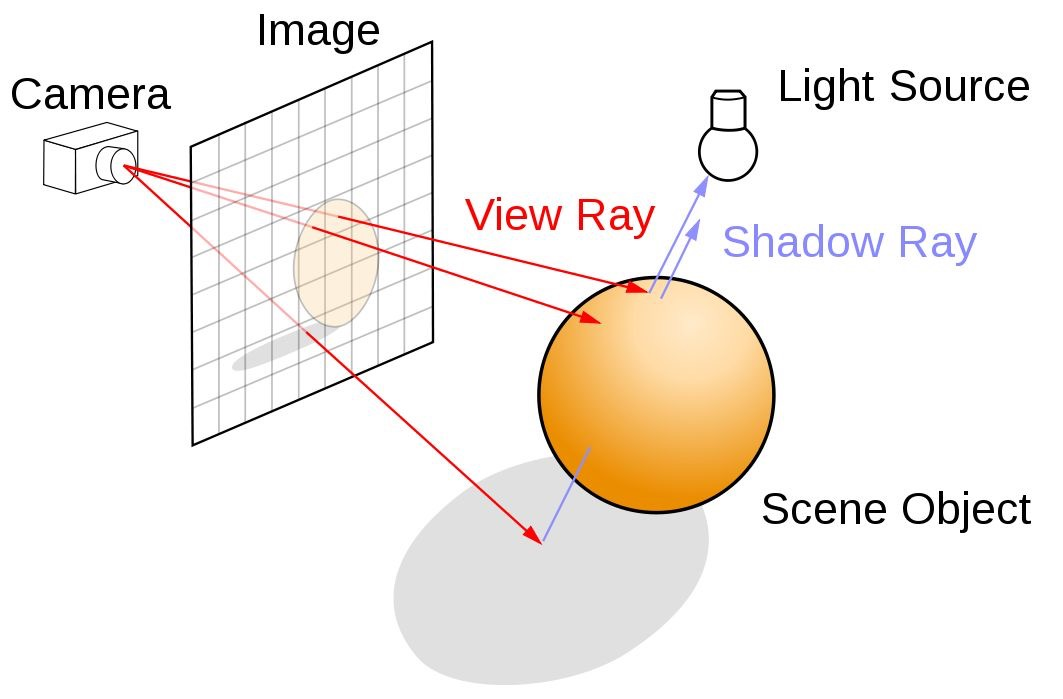
\includegraphics[width=\linewidth]{Images/ray-tracing-image-1.jpg}
   \caption{Ray tracing simulate the light's journey to compute the colour of each pixel on the rendered image.Image from [Henrik, 2008].}
   \label{fig:raytracing}
\end{figure}

Shooting only one ray per pixel can cause issues, such as jagged edges or missing tiny objects. To alleviate such issues, we can shoot multiple rays in a sub-pixel grid or in a random setting. However, this increases the render time because of the large number of computations required to trace the rays. This brings us to the trade-off between the render time and the accuracy of the rendered image. This trade-off often leads to different applications, such as virtual effects in the film industry requiring high accuracy with longer render time and real-time AR/VR applications with fast rendering but relatively low quality.

Ray tracing is a computationally expensive rendering technique that simulates the light transport realistically, following the laws of physics. Unlike rasterization, ray tracing does not deal with perspective projection or visibility explicitly or separately. Instead, it simulates both naturally by computing the intersection points of the ray with objects. Here, I explained the basics of the algorithm, which has advanced in recent years with intensive versions known as path tracing. 

\subsection{Shaders and BRDF}

Shading is the process of computing the colour of objects seen from the camera's viewpoint. Earlier, we discussed that achieving photorealism involves two main steps:  visibility along with perspective projection and shading. If we are to achieve photorealism, shading should reproduce the appearance of a scene so realistically that our eyes perceive the rendered image the same as the real word. A photorealistic image should look like a photograph of the same scene taken from the same viewpoint. 

Appearance is, in principle, the by-product of illumination and object properties. As the scene gets more light, objects are likely to appear brighter. Object properties that determine the appearance are reflectivity, which defines light-material interactions, and the geometric construction, i.e., orientation. The object colour we perceive is the mixture of light rays reflected off the surface. Objects often do not emit light but are lit by light sources emitting rays. This emitted light hits the surface of the object, some of which is later reflected off the surface and reaches our eyes, creating the object's colour. This type of lighting is known as direct lighting since the reflected light directly comes to our eyes after visiting the object. Indirect illumination occurs when an object gets some light reflected off other objects. Light can bounce off multiple surfaces, even infinitely many, before reaching our eyes.

Let's return to the discussion on lighting and shading effects we observe in the real world. We mentioned that what differentiates the objects with mirror-like,  specular and diffuse surfaces is the way they reflect the incoming light. A diffuse or Lambertian surface randomly spreads the incident light, looking equally bright in all viewing directions. Mirror-like objects reflect the ray around the point of contact, while specular surfaces distribute the light around the mirror direction. In the case of mirror-like or specular surfaces, the objects wouldn't be visible if our viewing direction is far from the mirror direction. Although we clearly distinguish different types of surfaces in computer graphics, real-world surfaces do not necessarily show only one kind of reflection.


Most real-world objects can exhibit both diffuse and specular reflections at the same time. This can happen either because the object is composed of multiple materials with different reflectivities joined together, or it has multiple layers of materials added on top of each other, as in the skin layers. Putting them together, we can define the overall appearance as the weighted sum of diffuse and specular components: 
\begin{equation}
I = k_d * I_d + k_s * I_s
\end{equation}
where $I$ is the total intensity of the light reflected by the surface at the point of contact, $I_d$ and $I_s$  are diffuse and specular intensities, and $k_d$ and $k_s$ are their corresponding coefficients. Here, we oversimplify the representation, neglecting shadows and interaction between objects.



\begin{wrapfigure}{l}{7.5cm}
  \centering
  % \fbox{\rule{0pt}{2in} \rule{0.9\linewidth}{0pt}}
   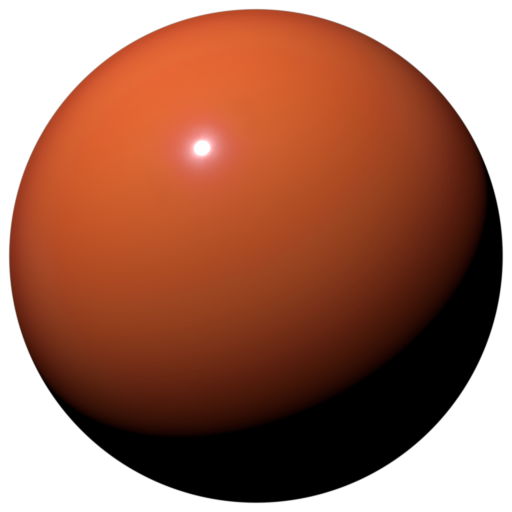
\includegraphics[width=0.5\linewidth]{Images/specular+diffuse.png}
   \caption{A material composed of both specular and diffuse components, lit by a point light source. The specular highlight (white circle) is centered around the light source direction. The material is specular-maroon-phenolic from MERL dataset \cite{Matusik2003jul}.}
   \label{fig:diffuse+spec}
\end{wrapfigure}


The diffuse shading can be computed based on the angle between the normalized incident light direction $L$ and the normal to the surface $N$:
\begin{equation}
I_d = I_l \, k_d \cos(\theta) = I_l \, k_d \, (N . L)
\end{equation}
where $I_l$ is the intensity of the light source. Note that the lights with different colours can have different $I_l$ and $k_d$. Also, $\cos(\theta) < 0$ indicates that the light remains behind the surface, not contributing to the brightness on the visible side. The effect of $\cos$ term is visible in Figure \ref{fig:diffuse+spec}, where the diffuse intensity gets dimmer as the points on the surface gets further away from the point of contact (specular highlight). 

\begin{figure}[ht]
  \centering
  % \fbox{\rule{0pt}{2in} \rule{0.9\linewidth}{0pt}}
   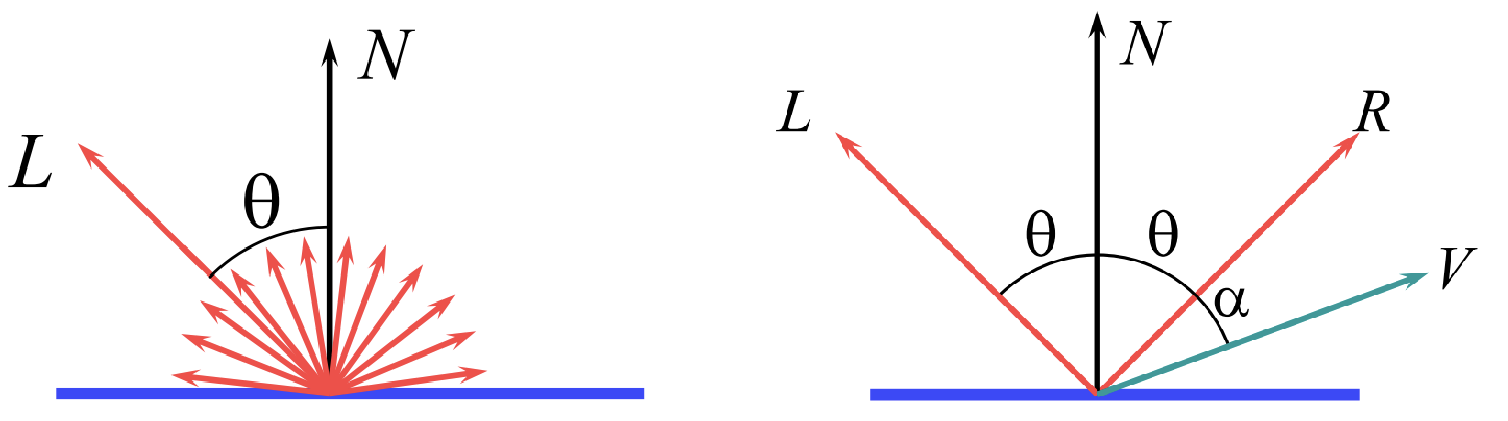
\includegraphics[width=\linewidth]{Images/diffuse+specular+angle.pdf}
   \caption{Diffuse and specular reflections.. Figures from [Mantiuk, 2022]}
   \label{fig:diffuse-spec-angle}
\end{figure}

Furthermore, the specular term can be approximated by:
\begin{equation}
I_s = I_l \, k_s \, \cos^n(\alpha) = I_l \, k_s \, (R . V)^n 
\end{equation}
where $R$ is the mirror reflection, $V$ is the viewing direction, and $n$ is an ad-hoc roughness coefficient (Figure \ref{fig:diffuse-spec-angle}).


We mentioned that the consideration of only diffuse and specular reflections ignores indirect lighting, which can be compensated by adding an additional constant term, $I_a * k_a$, known as ambient illumination. The overall shading then becomes:

\begin{equation}
I = I_a * k_a + \sum_i \, I_i \, k_d \, (N . L) + \sum_i \, I_i \, k_s \, (R_i . V)^n
\label{eq:Phong-eq}
\end{equation}

This mathematical model is known as the Phong shading model, a well-known shading model used for decades in computer graphics. The simplified specular reflection term was introduced by Phong in 1998 \cite{phong1998illumination}. This model does not take into account the shadows, requiring an additional ray tracing or shadow mapping for the simulation of shadows. It also considers the light sources infinitely far from the surface, ensuring the lighting direction $L$ remains the same across the surface.

Modelling light-material interactions is extremely complex due to the nature of materials. Hence, computer graphics researchers have developed mathematical models to approximate the function defining the reflectance of a material surface. This function is known as the Bidirectional Reflectance Distribution Function (\gls{BRDF}). The Phong shading model is one of the most popular BRDF approximation models due to its simplicity. Some other mathematical models include Cook-Torrance~\cite{cooktorrance1982}, Ward~\cite{ward1992} and GGX~\cite{walter2007microfacet}, with GGX being the most widely used approximation for its realistic results. I will compare HyperBRDF with GGX results in Chapter \ref{ch:HyperBRDF}.

Before going into the details of BRDF, let's examine the effect of the roughness term in the Phong model:

\begin{figure}[ht]
  \centering
  % \fbox{\rule{0pt}{2in} \rule{0.9\linewidth}{0pt}}
   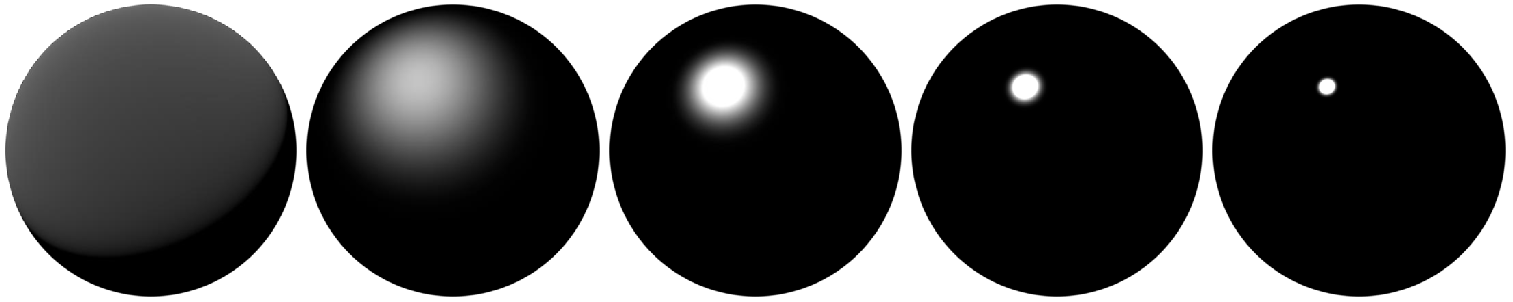
\includegraphics[width=\linewidth]{Images/Phong-roughness-coeff.pdf}
   \caption{Phong shading model implementation with decreasing roughness/increasing glossiness from left to right.}
   \label{fig:phong-roughness}
\end{figure}

\begin{wrapfigure}{l}{6cm}
  \centering
  % \fbox{\rule{0pt}{2in} \rule{0.9\linewidth}{0pt}}
   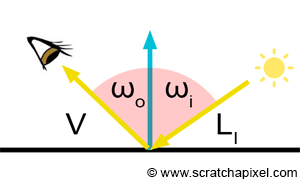
\includegraphics[width=\linewidth]{Images/shad2-brdfdir}
   \caption{BRDF depends on the incident light and viewing direction.}
   \label{fig:brdf}
\end{wrapfigure}
The rougher the material surface is, the more matte the object appears. As we decrease its roughness by increasing the value $n$, the specular highlight becomes a mirror-like reflection around the point of contact. 


\paragraph{BRDF.} 
Looking at Eqn. \ref{eq:Phong-eq}, we observe that the appearance/shading depends on two variables: incoming light direction for diffuse and specular terms and viewing direction for specular only. Therefore, we can generalise this function as a function with two parameters as  $f_R(\omega_o, \omega_i)$, where  $\omega_o$ and $\omega_i$ are the angles between the surface normal and viewing direction and the light direction, respectively (Figure \ref{fig:brdf}). This function, known as BRDF, gives us the amount of light reflected in the viewing direction when the surface is lit in the incoming light direction.

The mathematical formulations, such as Phong or GGX, approximate $BRDF(\omega_o, \omega_i)$s of real-world materials with simplifying assumptions on their nature. For instance, some models are designed to simulate only certain material types (Oren-Nayar model for Moon's BRDF). Some models follow the principle of optics or are designed empirically (Phong). Fitting to measured BRDF values is another alternative approach that recent neural network-based models, including HyperBRDF, are built upon.  

Comparing the mathematical approximations to real-world measurements helps us understand how accurate the BRDF model represents a real-world material. $BRDF(\omega_o, \omega_i)$ itself is defined based on the laws of physics and can be physically measured by some specialised hardware, such as gonioreflectometer. Cameras can also be used to measure the BRDF. For instance, the MERL dataset \cite{Matusik2003jul} is captured using a CCD camera. However, measuring the specular values can become a challenge with a camera capture due to the requirement of High Dynamic Range support. 


Real-world BRDF measurements are usually represented as tabulated data where each pair of incoming and outgoing directions corresponds to the brightness of RGB colours. In case the directions are defined in the Cartesian coordinates with $x, y, z$ values, the representation maps a six-dimensional input ($\omega_i, \omega_o$) to a three-dimensional output value (RGB colour). The precise representation of BRDFs requires densely sampled captures, such as more than a million samples in the MERL dataset \cite{Matusik2003jul} Consequently, a specialised hardware system measures the BRDF values at every small increments of the incoming and outgoing angles, covering a large range of possible values. 

It is worth mentioning that different approaches have been proposed to parametrise the BRDF as an alternative to the standard ($\omega_i$, $\omega_o$) parametrisation.  For instance, \citeauthor{rusinkiewicz1998new} \cite{rusinkiewicz1998new} replace ($\omega_i$, $\omega_o$)  with halfangle $\bm{h}$ and difference vector $\bm{d}$ for more efficient representations based on common BRDF features. In their proposed coordinate system, isotropic BRDFs become independent of halfangle. Furthermore, \citeauthor{dupuy2018adaptive} \cite{dupuy2018adaptive} propose an adaptive parameterisation that automatically adapts to the behaviour of a material. For the HyperBRDF experiments in Chapter \ref{ch:HyperBRDF}, I express the BRDFs using the Rusinkiewicz parametrisation \cite{rusinkiewicz1998new} for the efficiency in isotropic materials.


\begin{figure}[ht]
  \centering
  % \fbox{\rule{0pt}{2in} \rule{0.9\linewidth}{0pt}}
   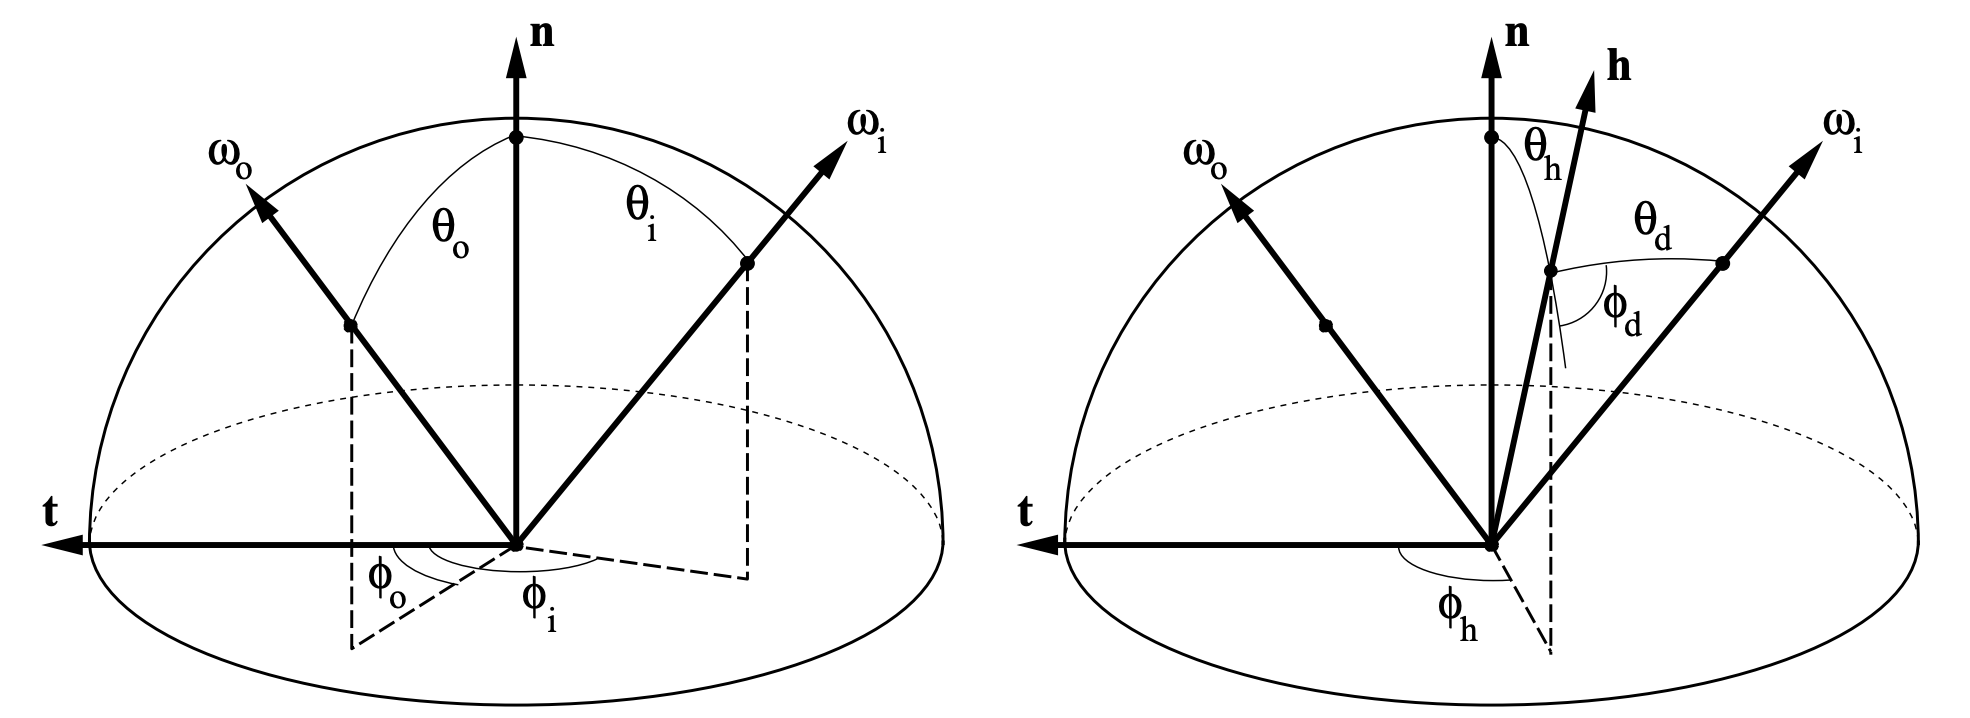
\includegraphics[width=\linewidth]{Images/Rusinkiewicz.png}
   \caption{Standard (left) vs Rusinkiewicz parametrisation. Figure from [Rusinkiewicz, 1998]}
   \label{fig:RusinkiewiczvsStandard}
\end{figure}


The BRDF is essentially a radiometric term with the usage in computer graphics for realistic simulations of light-material interactions. Hence, physically-based BRDFs hold the following properties:
\begin{itemize}
  \item positivity $f_R(\omega_o, \omega_i) \geq 0$, BRDF is positive across valid incoming and outgoing directions.
  \item Helmholtz reciprocity: $f_R(\omega_o, \omega_i) = f_R(\omega_i, \omega_o)$, The surface acts the same if the incoming and outgoing directions are switched.
  \item energy conservation. Unless the object emits light, the reflected light cannot be larger than the received one.
\end{itemize}


BRDF models should hold these physics-based properties to reproduce appearance realistically. In \citeauthor{Chenliang's paper} \cite{Chenliang's paper}, we discuss how these properties can be enforced in neural BRDF models. 

Rendering based on simulating the light's journey is computationally expensive. Therefore, a fast BRDF computation is an important consideration while choosing a model. For instance, Phong is a simple model that requires fewer computations. However, it is not energy-conserving. Recent mathematical models, such as GGX, have replaced Phong due to more accurate representations. Nevertheless, mathematical models still oversimplify the complex real-world BRDFs, constrained with a few parameters to tune. Therefore, recent work has started developing neural network-based approaches, which can offer higher capacity for the representation of highly-complex material appearance.

Lastly, we defined BRDF as the function of only two parameters, the incoming and outgoing directions, for which we assume that material properties remain the same across the whole surface. Complex real-world materials are composed of different substances, which results in showing various reflectivities at different points of contact. The Spatially Varying Bidirectional Reflectance Distribution Function (SVBRDF) can represent this behaviour with an additional location parameter ($f_R(\omega_o, \omega_i,  \vec{x})$). Furthermore, we assume that the reflected light leaves the surface at the point of contact, which unlikely occurs in translucent materials where we observe subsurface scattering. The Bidirectional Surface Scattering Reflectance Distribution Function (BSSRDF) represents such behaviour with additional parameters for both entry and exit locations ($f_R(\omega_o, \vec{x_o}, \omega_i,  \vec{x_i})$). For the rest of this thesis, I will only focus on BRDF representations with the assumptions mentioned here.

\subsection{Rendering equation}

To conclude the rendering section, let's define the rendering equation used to reproduce the outgoing light in ray tracing algorithms for the realistic simulation of light-material interactions.:
\begin{equation}
L_o(\vec{x}, \omega_o) = L_e(\vec{x}, \omega_o)  +  \int_S^2 L_i(\vec{x}, \omega_i) \, f_{\vec{x}}(\omega_o,  \omega_i) \, \abs{w_i . N} d\omega_i
\label{eqn:rendering-eqn}
\end{equation}
Here, $L_o(\vec{x}, \omega_o) $ is the outgoing light at point $x$ in the direction of $\omega_o$, $L_e(\vec{x}, \omega_o)$ is the emitted light that represents the light sources, $L_i(\vec{x}, \omega_i) $ is the incoming light at point $x$ in the direction of $\omega_i$, $f_{\vec{x}}(\omega_o,  \omega_i)$ is the BRDF, and $\abs{w_i . N} = \cos(\theta_i)$ is the Lambert's cosine term.

The rendering equation gives the outgoing light at point $x$ for a given incident light direction with the known BRDF. Here, we can define the BRDF term in multiple ways, such as with mathematical models discussed earlier, with a neural network outputting the BRDF values when fed with the directions or with physical measurements captured with special instruments. 

\section{Machine learning}
This section gives an overview of the machine learning techniques I have utilised for the appearance manipulation techniques proposed in the following chapters. Machine learning techniques have become the state-of-the-art approach in most computer vision and graphics tasks due to their promising ability to learn. Especially the advances in the field with the introduction of deep learning that offers inherent nonlinearity have made these models ideal for tackling ill-posed image editing tasks that most often have $many$ solutions.

Starting with the learning process, I will first discuss the basics of machine learning, including multilayer perceptrons that will build the baseline for the machine-learning framework proposed in one-shot detail retouching. Later, I will discuss neural representations that offer the storage of the data in a novel neural network-based setup, which is very useful for the processing of visual data that usually lies in a complex high-dimensional space. The hypernetwork model I borrowed for the HyperBRDF model is a neural representation model generalizable to new data for reconstruction. Lastly, I will summarise diffusion models, specifically latent diffusion, for zero-shot transient attribute transfer.

\subsection{Foundations}
Machine learning (ML) is a subfield of artificial intelligence (AI) in which machines learn a task from data without explicit programming. ML algorithms, such as linear regression, decision trees or neural networks, define the procedure for the learning process. An ML model is the trained version of the algorithm used to make predictions or decisions. The model consists of internal variables (parameters) learned during the learning process, known as training. The model structure is called architecture, which can include tree nodes, neurons, layers, connections, etc.

\paragraph{Types of learning.} The data is the key to the success of any ML algorithm. Supervised learning methods use paired data, each training example including input data and its corresponding output (label). The model learns a mapping between the input and the output. Classification or image-to-image translation can be given as examples. Unsupervised learning approaches, such as clustering or dimensionality reduction, learn patterns from the data without any label. Some methods, semi-supervised methods, combine both labelled and unlabeled data. Lastly, reinforcement models learn the task with a feedback mechanism, including rewards and punishments. The ML algorithms I have utilised for my main approaches are based on supervised learning. Therefore, the rest of this section focuses on supervised learning.

\paragraph{Training.} During training, the model learns from a dataset, that is, updates its parameters to minimise the errors in predictions with a loss function. Training is an iterative method and starts with assigning initial values to model parameters. These initial values are, in general, chosen to be random. At each iteration, \textbf{epoch}, the parameters are adjusted with an optimiser, such as gradient descent or Adam, that reduces the errors in predictions. The errors are computed for each training example and averaged over the training dataset for the epoch loss. 

The large amount of data in the training set can make parameter updates slow and computationally expensive. Therefore, the dataset is often split into subsets, known as \textbf{batches}, and each batch is processed separately at each epoch. The \textbf{batch size} is the number of training examples in one batch. It affects the efficiency, the stability of the model updates and the convergence speed. The completion of one epoch means that the model passed through the entire dataset once. The number of batches multiplied by the batch size gives the total number of examples in the training dataset. For instance, if we have a dataset of 100,000 images and choose batch size 1000, we then process 100 batches to complete one epoch. 

\begin{wrapfigure}{r}{7cm}
  \centering
  % \fbox{\rule{0pt}{2in} \rule{0.9\linewidth}{0pt}}
   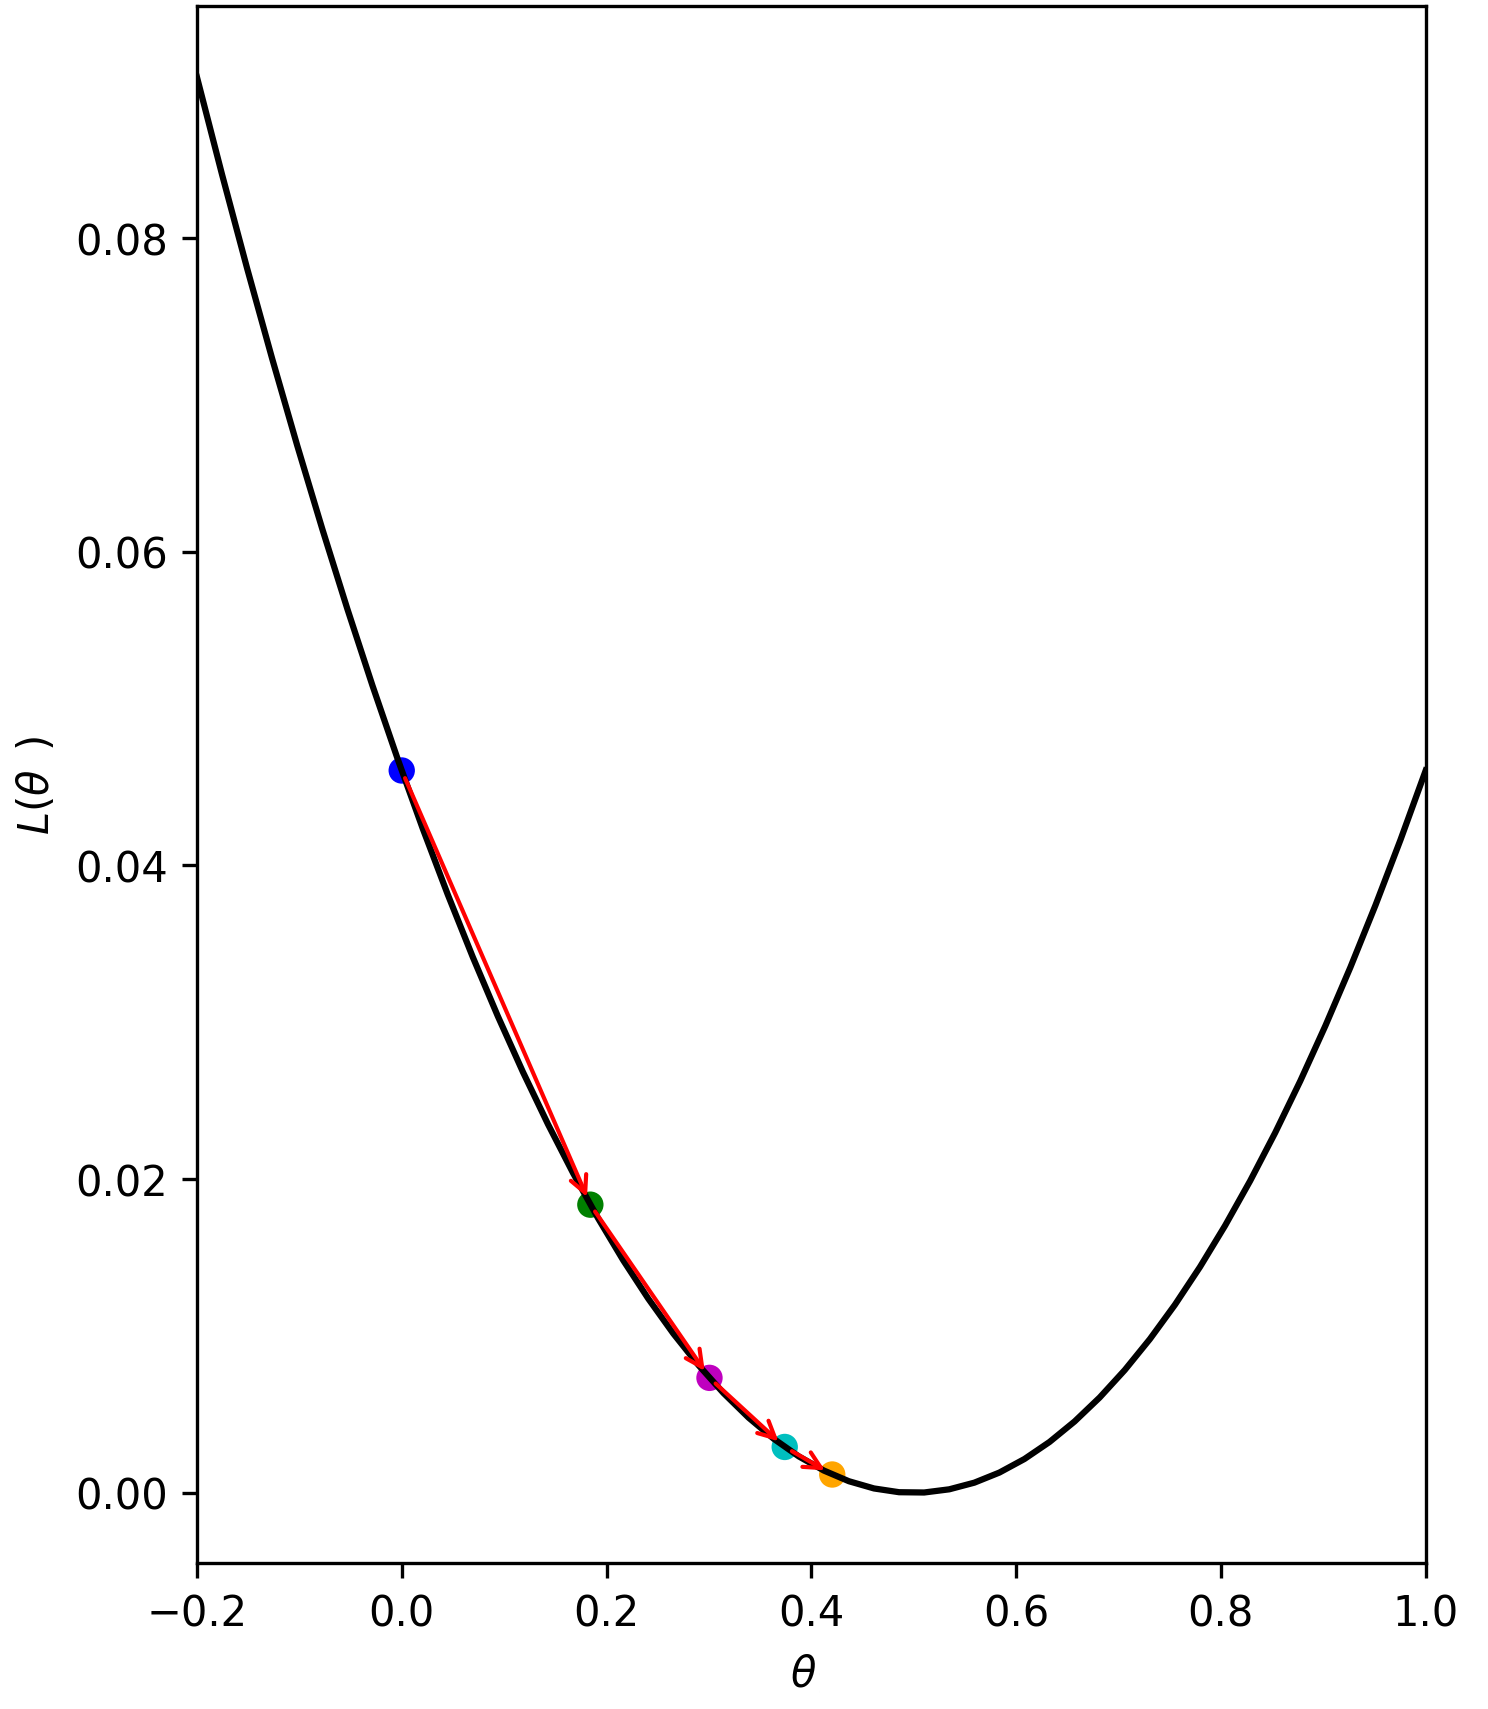
\includegraphics[width=\linewidth]{Images/gradient-descent.png}
   \caption{Gradient descent steps.}
   \label{fig:gradient-descent}
\end{wrapfigure}
The model parameters can be updated either after the entire dataset is passed through the model (\textbf{batch gradient descent}), or after each batch is processed (\textbf{mini-batch gradient descent}), or for one training example rather than waiting for batch or dataset processing (\textbf{stochastic gradient descent (\gls{SGD})}). The formula for the stochastic gradient descent is $\theta = \theta - \eta \, \nabla_{\theta} \mathcal{L}(\theta; x_i, y_i)$, where $\theta$ represents the model parameters, $\eta$ is the learning rate or step size, and $x_i$ and $y_i$ are the example input and its label, respectively. The term $\nabla_{\theta} \mathcal{L}(\theta; x_i, y_i)$ is the gradient of the loss function that directs the parameters towards the opposite of the derivative of the loss function. The drawback of the SGD is that the convergence may be slow and noisy due to high variance in updates. Therefore, Adam optimiser has surged as an alternative to SGD and gained more popularity among the ML research community. SGD keeps the learning rate $\eta$ the same for all parameter updates and across all epochs. Adam, on the other hand,  adapts an adaptive learning rate scheme and combines the advantages of two extensions of SGD: Adaptive Gradient Algorithm (AdaGrad) and Root Mean Square Propagation (RMSProp). It updates the learning rate for each parameter based on estimates of the first and second moments of the gradients. The adaptive learning rate scheme helps the model converge faster with higher performance. The extra information about Adam optimiser can be found in the main paper \cite{kingma2014adam}. For the results in the following chapters, I utilised the Adam optimiser while training the ML models.

The training settings, such as batch size, learning rate or number of epochs, change from task to task. These external settings, known as hyperparameters, are set before the training starts and control the flow of the training process. The hyperparameters are not learned from the data but need tuning with some techniques, such as grid search or Bayesian optimisation, for the best model performance. The size of the model also depends on the task. For a large-scale project, such as text generation, a model might require millions of parameters for effective results. However, we can also learn a handful of parameters. For instance, fitting the real-world BRDF measurements to mathematical models only requires learning 3-5 parameters. One-shot detail retouching also proposes trainable transformation matrices of size $9 \times 9$ whose entries are learned during training.

\paragraph{Loss function.} We mentioned that the optimiser tries to minimise the errors in predictions with a loss function. In supervised learning, the loss can be defined as the difference between the model output and the label, also known as ground truth. Defining the difference depends on the expectations from the model. Two well-known loss functions are L1 and L2 norm distances. If we define the neural network as a function $f_\theta$, then L1 loss becomes $\mathcal{L}_{1} = \sum_i \,\abs{y_i - f_\theta(x_i)}$, and L2 loss is $\mathcal{L}_{2} = \sum_i \, (y_i - f_\theta(x_i))^2$ (Figure \ref{fig:l1vsl2loss}).  If the dataset consists of outliers, data points that significantly diverge from the remaining data points, L2 leads to larger errors due to the computation of the squared differences. For instance, details or high-frequency components in an image can be considered outliers as these values deviate from the average image. Therefore, L1 loss might be more handy for enhancing the details. If the losses are averaged over the dataset, they are called Mean Absolute Error (MAE) and Mean Squared Error (MSE), respectively.

Some tasks might require more sophisticated loss functions. For instance, we can compute the difference on another space by first projecting the paired data onto the target space. VGG loss \cite{johnson2016perceptuallossesrealtimestyle} uses a VGG network to map the input image to their style features, which are then used to compute the L2 loss. In HyperBRDF, I first apply a logarithmic mapping to scale the data for more effective training. Such tricks are, in general, task-specific and are designed to improve the model performance.


\begin{figure}[ht]
  \centering
  % \fbox{\rule{0pt}{2in} \rule{0.9\linewidth}{0pt}}
   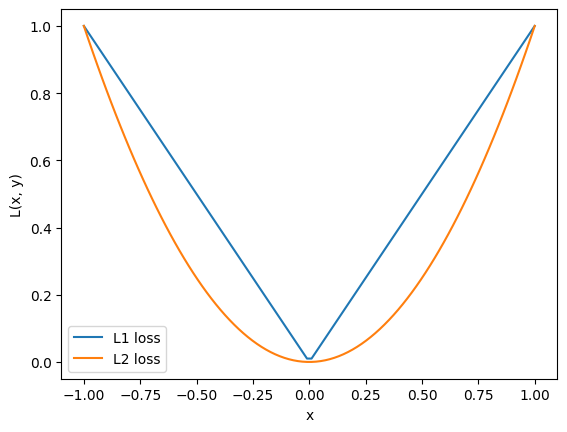
\includegraphics[width=0.6\linewidth]{Images/l1vsl2loss.png}
   \caption{L1 vs L2 loss values for a single data point. Ground truth $y$ is set to 0.}
   \label{fig:l1vsl2loss}
\end{figure}

\paragraph{Regularisation.} Training the model on the entire dataset can lead to overfitting. That is, the model's performance significantly decreases when tested on different data points. It occurs when the learned model becomes highly complex, no longer representing the overall data distribution but fitting to individual training samples instead. To make models generalise well to new data, we can add a regularisation term to the loss function. This term helps penalise the highly complex models, preventing overfitting. L1 ($\lambda \, \sum_i \abs{\theta_i}$) and L2 norm ($\lambda \, \sum_i \theta^2_i$) regularizations are two well-known terms. L1 norm pushes low parameter values to zero, encouraging sparsity. As some parameters become zero, L1 regularisation becomes highly effective in feature selection. L2 regularisation reduces model complexity but maintains the features. It manages multicollinearity by distributing the importance among correlated features and offers smooth solutions. The coefficient $\lambda$ defines the strength of the regularisation. If we combine a MSE with L2 regularisation, we will have the following loss function:

\begin{equation}
\mathcal{L}(\theta) = \frac{1}{m} \sum_{i=1}^{m} (y_i - f_\theta(x_i))^2 + \lambda \sum_{j=1}^{n} \theta_j^2
\label{MSE-with-L2reg}
\end{equation}

Here, $m$ is the number of training samples, and $n$ indicates the number of parameters. In HyperBRDF, I benefitted from L2 regularization for both latent representations and model parameters to maintain the features while reducing collinearity.

\paragraph{Data augmentation} is the process of producing altered versions of pre-existing data samples with the aim of increasing the diversity in the training dataset. Data augmentation is another strategy to prevent overfitting and make the model more generalizable to new samples. It also helps compensate for data-scarce regimes where collecting a large-scale dataset is highly impractical. The augmentation approach depends on the type of data. For images, the types of augmentation can include geometric transformations, such as rotating, scaling, translation, flipping, and cropping; colour space transformation, such as brightness, contrast, saturation and hue adjustment; noise injection; applying kernel filters; etc. In one-shot detail retouching, I extracted patches of size $3 \times 3$ with a stride of 1, which led to overlapping patches as a means of data augmentation.

\subsection{Multilayer perceptrons}

Inspired by biological neural networks, deep neural networks (DNN) are designed as artificial neural networks that consist of layers, neurons, and connections between the neurons. As the ML field has advanced over time, the neural network models have become highly complex with multiple layers that lie between the input and output layers. To understand the basics of DNNs, consider a linear equation $y = \sum^n_i\vec{w_i} . \vec{x_i} + b = \vec{w}^T . \vec{x} + b$, where neurons are input data points $x_i$ that are connected to the output neuron $y$ via connections, known as weights $w_i$ (Figure \ref{fig:neuron}), and a bias term $b$. Here, we have the input layer (first layer with input neurons) and the output layer (last layer of the network)  and weights multiplied with input data points to obtain the output. This model can be considered a basic neural network architecture. 

\begin{wrapfigure}{r}{5cm}
  \centering
  % \fbox{\rule{0pt}{2in} \rule{0.9\linewidth}{0pt}}
   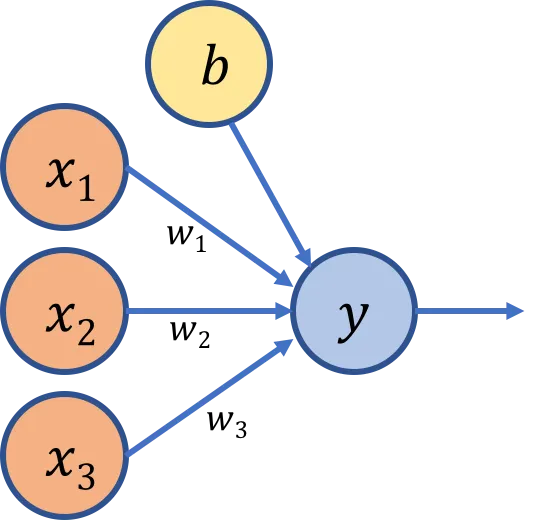
\includegraphics[width=\linewidth]{Images/neuron.png}
   \caption{Graph representation of a linear equation. Figure from [Issac, 2018].}
   \label{fig:neuron}
\end{wrapfigure}

The machine learning bit of neural networks is known as deep learning, a subfield of ML in which the learning process discussed above is used to learn the weights and biases of this equation or, more generally, the neural network. I mentioned earlier that nonlinearity is an inherent feature of deep learning. This comes from an additional function, known as the activation function, applied to the linear equation above ($y = \sigma(\vec{w} ^T. \vec{x} + b)$). The nonlinearity helps bring additional information to the linear system, which, otherwise, could have infinitely many solutions in the linear space.


With the assumption of a feedforward structure, a neural network can put its neurons into stacks of layers, each layer only depending on the previous layers. This model, a \textbf{multilayer perceptron (\gls{MLP})} (Figure \ref{fig:mlp}), is one of the simplest and most widely used neural network models that can be employed for multiple applications, such as image classification, regression, and pattern recognition. By extending the equation above, an MLP layer can be expressed in the matrix form as:
\begin{equation}
\vec{y} = \sigma \biggl(\mathbf{W}\vec{x} + \vec{b} \biggr)
\end{equation}
where $\mathbf{W}$ and $\vec{b}$ are the weight matrix and bias vector of the corresponding MLP layer. We can stack multiple such layers (hidden or intermediate layers) between the input and output layers, which increases the \textbf{depth} of the MLP:
\begin{equation}
\vec{y} = \sigma_2 \biggl( \mathbf{W}_2\sigma_1 \biggl(\mathbf{W}_1\vec{x} + \vec{b}_1 \biggr) + \vec{b}_2\biggr) 
\end{equation}
Here, each layer has its own weights and biases, weights multiplied by the output of the previous layer. We can compute the total number of parameters by multiplying the number of input and output neurons for each layer and then adding them all together along with the bias terms. 

%For instance, the total number of parameters in the MLP model shown below is $4 \times 5 + 5 \times 3 + 3 \times 2 + 5 + 3 + 2$.


\begin{figure}[ht]
  \centering
  % \fbox{\rule{0pt}{2in} \rule{0.9\linewidth}{0pt}}
   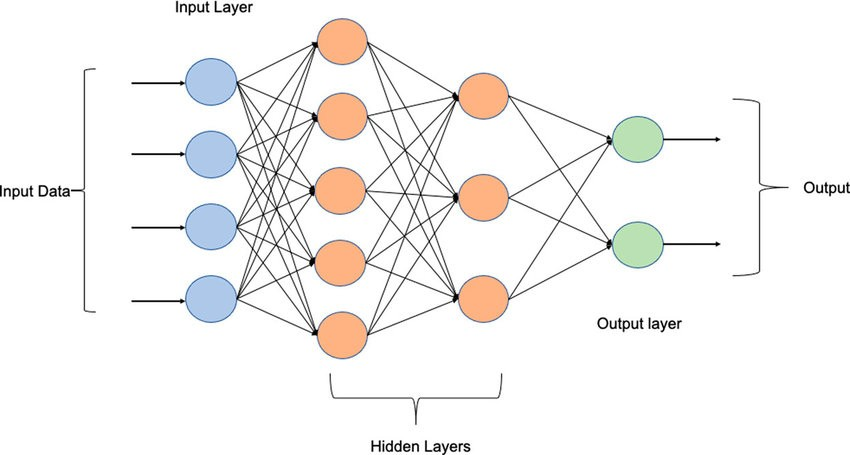
\includegraphics[width=\linewidth]{Images/MLP.jpeg}
   \caption{A basic multilayer perceptron model. Figure from [Kishore NG, 2023].}
   \label{fig:mlp}
\end{figure}

The passing of the input towards the network to obtain the output is called \textbf{forward pass} or \textbf{forward propagation}. The \textbf{backward pass}, on the other hand, defines the training process of neural networks. Training in deep learning follows the same steps as discussed earlier for the ML model training. We compute a loss function based on the output obtained with the forward pass, then take its gradients to update the parameters (weights and biases in this case). As deep neural networks have multiple layers, computing the gradient of the loss with respect to the first layers requires applying the chain rule. The gradients propagate back towards the input. That is why backward pass is also called \textbf{backpropagation}. One problem with backpropagation is that the gradients can get extremely small as they backpropagate towards the input layer, known as \textbf{vanishing gradients}. It happens because the gradient with respect to early layers is the product of the gradient with respect to later layers. If the gradient in the last layers is smaller than one, their products vanish rapidly. ReLU activation function, batch normalization, skip connections and gradient scaling are methods to overcome the vanishing gradients problems.

\paragraph{Activation functions.} The choice of activation functions depends on the task and output expectations. The ones I utilised for this dissertation are as follows:

\begin{itemize}
\item The rectified linear function (ReLU):

\begin{equation}
\sigma(x) = max(x, 0)
\end{equation}

ReLU is one of the most commonly used activation functions in computer vision problems due to the lack of vanishing gradients and computational efficiency. It is also an ideal choice when the output values should not go below zero. For instance, the value range of image pixels is, in general, $[0, 1]$ after pre-processing, or the BRDF values should hold positivity.

\item The exponential linear unit (ELU):
\begin{equation}
 \sigma(x) = \begin{cases}
x, & \text{if $x>0$}\\
\exp(x) - 1,  & \text{if $x\leq0$} 
  \end{cases}
\end{equation}

\item Sinusoidal Activation Function:

\begin{equation}
\sigma(x) = \sin(x)
\label{eq:sine-act}
\end{equation}
\end{itemize}

\subsection{Neural implicit representations}

At the beginning of this chapter, I discussed the limitations of the image display and representation due to discretisation. The real world is in a continuous spectrum, including geometry, light, reflectivity, and sound. However, we should discretise the inherently continuous signals for virtual representations and storage in computers. For example, images are represented as a grid of pixels, geometry as point clouds or meshes, and sound waves and electrical signals as discrete samples. The discrete representation bounds the amount of information about a signal to a discrete structure of a certain size. Not only scaling up an image does not bring any additional information but also causes artifacts, such as blurring or aliasing. 

To represent signals in a continuous domain, imagine we have a continuous function $f$ that maps the coordinates or locations to corresponding signal values. In an image case, the function $f$ takes $(x, y)$ pixel coordinates as input and outputs the corresponding RGB pixel value. This representation allows us to sample pixel grids at any resolution. More generally, the parameterisation of a signal as a mathematical formula offers a mapping from the coordinate space to the value space without resolution limitations. The difficulty with such a representation is to find the appropriate function since most signals are usually too complex to be analytically tractable. Neural implicit representations address this by representing signals with neural networks as they are essentially universal function approximators \cite{cybenko1989approximation}.

Recent advancements in computer vision and graphics research have transitioned from discrete representations to continuous function representations parameterised by multilayer perceptrons. These MLPs, also referred to as "coordinate-based" MLPs, utilise low-dimensional coordinates as inputs and are trained to output representations of shape, density, and/or colour at each respective input location \cite{ffn}. Their highly efficient compactness compared to grid-sampled representations as well as suitability for gradient-based optimisation make coordinate-based MLPs ideal for neural representations of signals. These MLPs have been employed to represent images \cite{nguyen2015deep}, volume density \cite{mildenhall2021nerf}, signed distance functions \cite{park2019deepsdf}, and BRDFs \cite{sztrajman2021neural}, achieving state-of-the-art performance across a range of tasks including shape and appearance representation, texture synthesis, and novel view synthesis.

ReLU-based MLPs are known to have a spectral bias \cite{rahaman2019spectral}. That is, they struggle with predicting high-frequency components, mainly fitting to low-frequency ones. This spectral bias causes losses in details, and consequently, the represented signals become blurry. To enhance the capacity of MLPs for highly accurate representations, methods based on sinusoidal functions have been proposed. In NeRF, a positional encoding with $cos$ and $sin$ mapping is applied to the continuous 5D coordinates (spatial location $(x, y, z)$ and viewing direction $(\theta, \phi)$) before feeding them to the network for novel view synthesis. \citeauthor{ffn} \cite{ffn} later shows that positional encoding is a special case of Fourier features \cite{rahimi2007random} and proposes a more general mapping formula that can be applied across a range of different tasks, including image and 3D shape regression and MRI reconstruction. Along this line, \citeauthor{sitzmann2020siren} \cite{sitzmann2020siren} propose replacing ReLU activation functions with a sinusoidal one (Eqn. \ref{eq:sine-act}).

Fourier feature mapping function $\gamma$ maps input points $\mathbf{v}$ to a higher dimensional space with a set of sinusoid:
\begin{equation}
\gamma(v) = [\alpha_1 \cos(2 \, \pi \, \mathbf{b}^T_1 \, \mathbf{v}), \alpha_1 \sin(2 \, \pi \, \mathbf{b}^T_1 \, \mathbf{v}), ..., \alpha_1 \cos(n \, \pi \, \mathbf{b}^T_n \, \mathbf{v}), \alpha_1 \sin(n \, \pi \, \mathbf{b}^T_n \, \mathbf{v})]
\label{eq:ffn}
\end{equation}

where $b_i$ and $a_i$ are considered as  the Fourier basis frequencies and the corresponding Fourier series coefficients, respectively.

\begin{figure}[ht]
  \centering
  % \fbox{\rule{0pt}{2in} \rule{0.9\linewidth}{0pt}}
   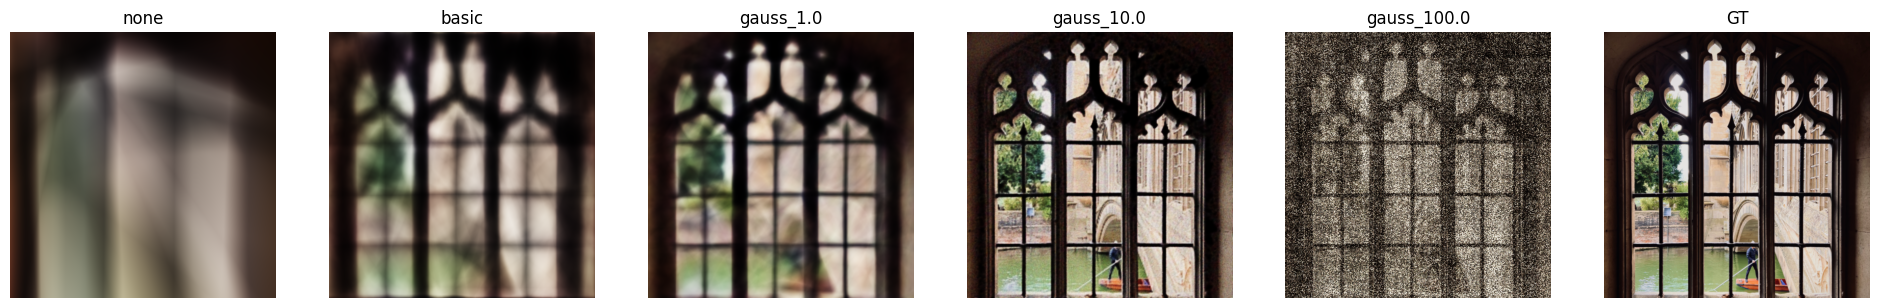
\includegraphics[width=\linewidth]{Images/FFN.png}
   \caption{To overcome the spectral bias in coordinate-based MLPs, a Fourier feature mapping \cite{ffn} can be applied before feeding the input to the model. Here, 'none' represents an MLP model without mapping. 'basic' and 'gauss' are different variants of Fourier feature maps, and 'GT' is the ground truth.}
   \label{fig:ffn}
\end{figure}

\paragraph{Generalisable neural implicit representations.}
The effectiveness of the coordinate-based MLP models with periodic functions either as an activation or a mapping is compelling. However, the drawback of such neural representations is that they are designed for the reconstruction of individual signals, which significantly reduces their generalisation capacity due to overfitting. One approach to convert these overfitting neural implicit representations to generalisable representations where a set of signals lies on a joint manifold is to condition the coordinate-based MLPs with a latent code that represents the location of a signal on the manifold. Concatenated latent vectors, hypernetworks, and attention-based set latent representations are three common approaches to such conditioning strategies \cite{rebain2022attention}.

Generalisable neural implicit representations have two main components: an encoder that learns the latent space representations of the signals and a decoder that maps to signal values. The conditioning mechanisms are a part of the decoder where the input coordinates and latent codes are both used to estimate the corresponding signal value. One option is to concatenate the latent code and input coordinates (either with or without any mapping) and feed this concatenated input to the MLP (Concatenated latent vectors). Another option is to use the latent code to predict the parameters of the coordinate-based MLP, whose input still remains the input coordinates (Hypernetworks). Alternatively, one can benefit from cross-attention layers which compute attention between a query related to the input coordinates and a batch of tokens which is equivalent to the latent codes (Attention-based conditioning). 


\begin{figure}[ht]
  \centering
  % \fbox{\rule{0pt}{2in} \rule{0.9\linewidth}{0pt}}
   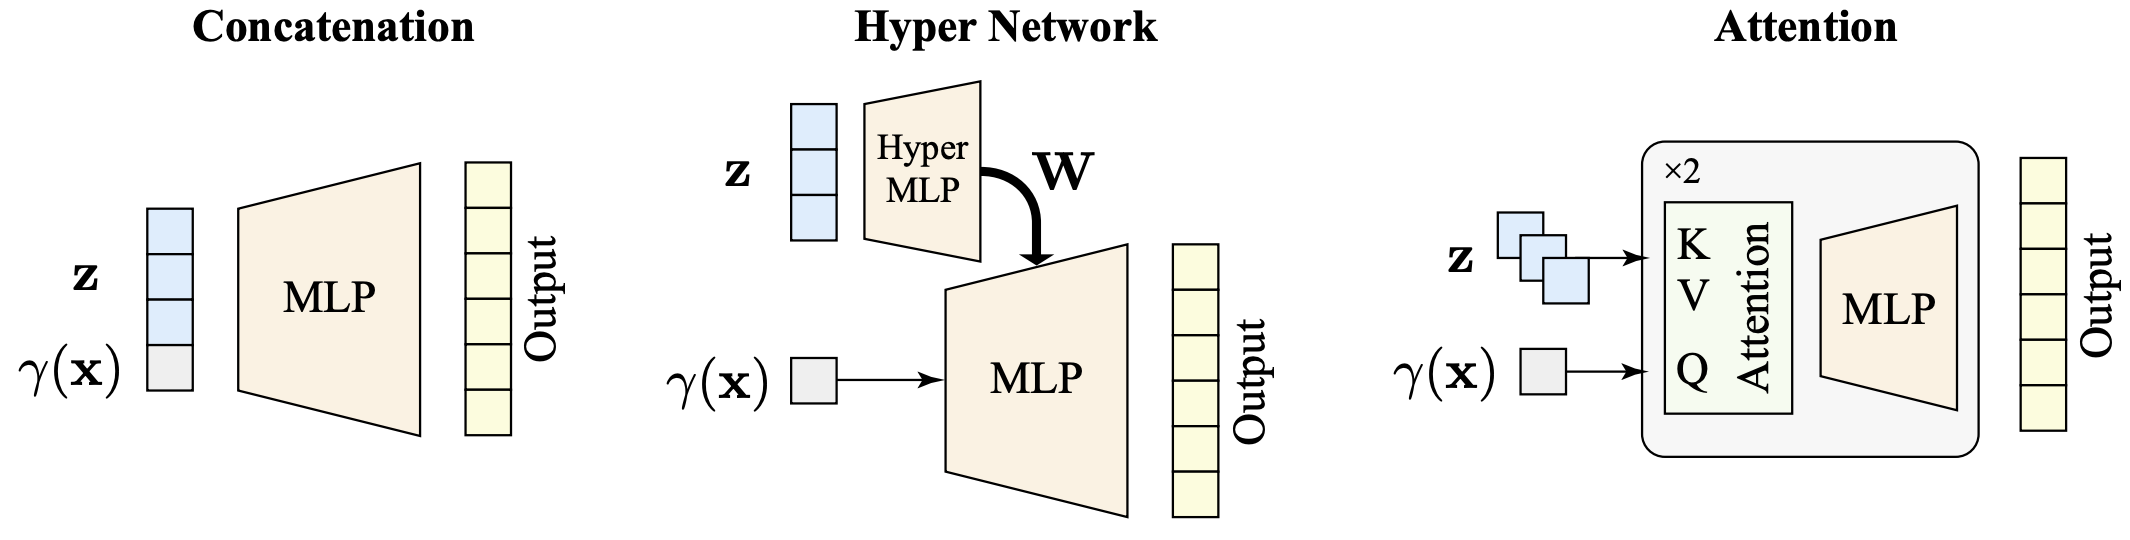
\includegraphics[width=\linewidth]{Images/conditioning-mechs.png}
   \caption{Three conditioning mechanisms for generalisable neural representations. Coordinate-based MLPs can be conditioned by 1) the concatenation of input coordinates \textbf{x} and latent code \textbf{z} (left), 2) another neural network predicting the weights of the primary MLP which takes the inpur coordinates as the input (middle), or 3) attention layers with a set of tokens (\textbf{z}) and coordinate-related query . Here, $\gamma$ is the mapping function discussed earlier and an optional component. Figure from [\citeauthor{rebain2022attention}, \citeyear{rebain2022attention}]}
   \label{fig:ffn}
\end{figure}


The joint representation of multiple signals helps learn a strong prior about common features of the signals, which can then be used to reconstruct individual signals effectively. For instance, HyperBRDF benefits from the learned prior about general material appearance so that it can reconstruct individual materials from a significantly reduced number of samples.  



\subsection{Diffusion models}
Diffusion models have emerged as an alternative to generative adversarial networks (GAN) and variational autoencoders (VAE) on the image generation domain and recently surpassed their performance in related computer vision tasks, such as conditional generation and image-to-image translation. 
\chapter{One-shot Detail Retouching}\label{one-shot}

Whether it is a human face we are examining or a butterfly wing with colourful tiny structures, details are the essential components defining aesthetics and identity. They drop hints about several aspects of the subjects, such as wrinkles pointing to either the rough age of the person or their emotional status, scratches describing the roughness of a material surface, or flyaway hair strands implying windy weather. When we capture a close-up photograph of a real-world scene, these details dominate the overall vibe of the scene, which consequently reflects on the appearance in photographs. As tiny as they are, however, editing these details is extremely challenging with a data-efficient learning-based approach due to the scarce number of pixels belonging to fine details. This chapter explores a detail editing task, photo retouching, and presents a novel learning-based framework that learns the transfers in intricate details from a single example pair.

Photo retouching is a challenging task for novice users, as it requires expert knowledge and advanced tools. Photographers often spend a significant amount of time producing high-quality retouched photos with intricate details. This chapter introduces a one-shot learning-based technique to automatically retouch details of an input image based on just a single pair of before and after example images. This approach provides accurate and generalisable detail edit transfer to new images, utilising a new representation for image-to-image maps. Specifically, I present neural field-based transformation blending in the patch space, which defines patch-to-patch transformations for each frequency band. This parametrisation of the map, with anchor transformations, associated weights, and spatio-spectrally localised patches, allows us to capture details effectively while remaining generalisable. I evaluate the proposed technique on both known ground truth filters and artist retouching edits. Our method accurately transfers complex detail retouching edits.

\begin{figure}
  \includegraphics[width=\textwidth]{Chapters/detail-retouching-figs/teaser_CVMP.pdf}
  \caption{The one-shot technique automatically transfers retouching edits to new images by learning the desired edits from one example \textit{before-after} pair (insets). The transferred edits accurately shape intricate details such as wrinkles, dark spots, strands of hair, or eyelashes, as shown in the input (top) and retouched (bottom) pairs. Images from [Jenavieve (top-left), Logan ProPro (top-left, inset), Marissa Oosterlee (top-middle). (CC-BY)].}
  % \Description{Our technique automatically transfers retouching edits to new images by learning the desired edits from one example \textit{before-after} pair (insets). The transferred edits accurately capture intricate details such as wrinkles, dark spots, strands of hair, or eyelashes, as shown in the input (top) and retouched (bottom) pairs.}
  \label{fig:teaser}
\end{figure}


% \received{20 February 2007}
% \received[revised]{12 March 2009}
% \received[accepted]{5 June 2009}






\section{Introduction}\label{sec:introduction}

Photo retouching is often desirable as it improves the aesthetic quality of photographs by eliminating imperfections and \nobreak highlighting subjects of interest. Even with significant progress in digital photography owing to advancements in camera sensors and image processing algorithms, professional retouches via manual adjustments are still needed to achieve a desired look. These artistic edits require considerable manual effort as they consist of global adjustments, such as brightening and contrast enhancement, as well as fine edits applied to local regions. Professionals spend a great deal of time to generate such edits, which motivates us to automatically mimic a specific style or type of retouch.

The development of automatic photo retouching tools can be helpful for both novice users and experts as it offers a basis for a professional retouching style. However, automating detailed edits of professionals is challenging as their editing pipelines are spatially varying, context-aware, and highly nonlinear, containing per-pixel adjustments. Recent learning-based methods address this complexity in image-to-image translation by proposing local context-aware methods, such as pixel-adaptive neural network architectures \cite{shaham2021spatially, li2020lapar}, learning parameters of local filters \cite{moran2020deeplpf}, or multi-stream models to extract global and local features separately \cite{Gharbi17Deep}. However, these data-driven methods require a large dataset of matching example image pairs. Even then, the mappings are sensitive to segmentation errors, unseen semantic regions, and image content~\cite{yan2016automatic}. %Many successful methods require example and input images to be content-wise pixel-level aligned to achieve plausible results \cite{Shih14Style}.

% in intricate details 
The gap between manual and automatic enhancement motivates me to develop a novel photo retouching technique that can learn global and local adjustments from just \emph{a single example image pair}. The proposed method thus sidesteps the need for large datasets, which are very difficult to obtain for the detail retouching task. Users are allowed to choose one example \emph{before-after} pair from which the model learns the underlying retouching style. Subsequently, the retouching edit can be applied to a different input image.

Here, we assume that example and input images share similar local content. The user can thus decide on the semantics of the example and input photos and the structural changes to be transferred. This is easy for humans and practical for many scenarios, e.g. face edits transferred to faces. The framework then handles the difficult part for humans: capturing how fine details change in an edit and applying those automatically to a new image. The method can further be combined with brushes if fully automatic transfers are not desired. 

This is achieved by defining the retouching problem as a map given by a \emph{spatio-spectral patch-space neural field based transformation blending}. This representation is primarily inspired by professional detail retouching pipelines as I elaborate on in Section \ref{chap:motivations}. This map representation is composed of learned patch maps at multiple scales, i.e. frequency bands. Each of these maps is represented by a number of \emph{transformation matrices} blended with \emph{patch-adaptive weights} that are learned by a multilayer perceptron. I jointly optimize the transformation matrices and corresponding weights for each band. This representation captures edits to details better than any previous techniques while staying generalizable to new images. It is also simple enough to be extended in many different ways in future works.

In summary, there are two main contributions of this work: 

%Multiple Transformation Blending
\begin{itemize}

    \item \textbf{A novel patch-space image map representation} as a weighted blending of transformation matrices with neural fields.
    
	\item \textbf{A one-shot detail retouching algorithm} that allows transfer of edits to details to new images based on a single before-after image pair.

\end{itemize}


\section{Related work}

Photo retouching has been explored in image processing and computer vision communities under different domains, such as photo enhancement and image-to-image translation. Below, we first discuss recent methods on photo enhancement and then image-to-image map definitions with the main focus on learning-based methods.

\subsection{Digital photo enhancement}
% \myworries{Check Rafals' paper -- is it global tone mapping, where to put it in the related work}
\paragraph{Global image enhancement.} Colour and tone transfer has been considered a very effective technique to improve the perceptual quality of photos with pre-defined rules or examples \cite{Faridul14ASurvey, mustafa2022distilling}. 

Earlier methods typically apply global changes and adjust image statistics \cite{Bychkovsky11Learning, Bae06Two, Pitie05NDimensional,Pitie07Automated,Reinhard01Color,Sunkavalli10Multi, he2020conditional, park2018distort}, e.g., mean and standard deviation, without considering image content and local variations \cite{CohenOr06Color}. These methods, in general, transfer colour changes, ignoring edits in fine details. On the other hand, the proposed method learns a mapping per frequency band, capturing transfers even in high frequencies. \citeauthor{Bychkovsky11Learning} \cite{Bychkovsky11Learning} collected the MIT-Adobe FiveK dataset of 5,000 photographs and their retouched versions by five artists. The authors propose a regression model to learn artists' retouching styles from before-retouched pairs. \citeauthor{chen2017fast} \cite{chen2017fast} introduce a fully-convolutional neural network model to learn global image processing operators, such as photographic style, nonlocal dehazing, and pencil drawing. \citeauthor{Hu18Exposure} \cite{Hu18Exposure} presents a photo retouching pipeline for various post-processing operations, where global adjustment curves are approximated. The authors propose a deep reinforcement learning approach to model users' edit preferences from a given photo collection. 
 
Nevertheless, global transfers cannot capture local and regional variations in a photo \cite{CohenOr06Color}.They may result in artifacts when the local target regions of the example and input images do not match. In this method, we adapt the mappings to each image patch separately, thus accurately capturing local edits in intricate details.

\paragraph{Local context-aware image enhancement.} 
 To capture local variations, different methods have been proposed, such as learning local representative color transform \cite{kim2021representative}, estimating an image-to-illumination mapping with a local feature extractor \cite{wang2019underexposed}, local histogram matching \cite{Shapira13Image}, segmentation \cite{Laffont14Transient,Tai07Soft}, combining and learning pre-defined filters \cite{Berthouzoz11AFramework,Chen18Deep,Huang14Parametric,Omiya18Learning,Saeedi18Multimodal} or with further user guidance \cite{An10User,Pouli11Progressive,Tai05Local}, detection or learning of image semantics and context \cite{Gharbi17Deep,Hwang12Context,Kaufman12Content,Nam17Deep,Yan14Automatic,Zhu18Automatic}, matching \cite{HaCohen11Nonrigid}, or precise alignment \cite{Kagarlitsky09Piecewise, Shih13Data}. 
 
 Furthermore, recent work has focused on learning global and local adjustments via spatially-varying filters \cite{moran2020deeplpf, Gharbi17Deep, chen2018deep, shaham2021spatially, li2020lapar}. \citeauthor{chen2018deep} \cite{chen2018deep} introduce a global feature extraction layer along with per-pixel adjustments to enhance photos. Bilateral guided joint upsampling \cite{chen2016bilateral} also allows for local and global image processing with an encoder-decoder approach. HDRNet \cite{Gharbi17Deep} learn content-aware, global, and local adjustments via a two-stream convolutional architecture, which extracts local and global features separately to fit local affine transformations and encode the high-level description of images, respectively. Also, \citeauthor{moran2020deeplpf} \cite{moran2020deeplpf} propose to learn the parameters of three different spatially local filters to automatically enhance photos. 

Local color and tone adjustments might still be insufficient to capture intricate details \cite{Bae06Two}. Transfer of such details typically requires a dense matching \cite{HaCohen11Nonrigid} or alignment between example and input images \cite{Shih14Style}. To achieve either dense matching or alignment, methods constrain their datasets to contain very similar example and input images, for example, faces with similar characteristics and views~\cite{Shih14Style}. On the other hand, this framework does not require dense correspondences between input and example images but still transfers intricate details. It accurately represents such complex mappings with an operator summing the effects of various transformations multiplied with corresponding patch-adaptive weights, applied at multiple frequency bands.

\paragraph{Differentiable image processing pipelines.}
To have more flexibility and control over the rendering process, methods based on image signal processors (ISP)s have been proposed to enhance photos. In both \cite{tseng2019hyperparameter, yu2021reconfigisp}, hyperparameters of an ISP are optimized. Different from \cite{tseng2019hyperparameter}, which only applies to a fixed pipeline, \citeauthor{yu2021reconfigisp} \cite{yu2021reconfigisp} can explore different ISP architectures. Furthermore, \citeauthor{tseng2022neural} \cite{tseng2022neural} model a commercial raw processing pipeline with a series of neural networks to render sRGB images from raw inputs. As we assume example and input images to be processed RGB images rather than raw data, I refrain from comparing our method with such ISP-based methods.


\subsection{Defining maps between images}

\paragraph{Unsupervised methods.} Some learning-based techniques only require one or more examples of retouched photos without their before examples to learn the transfer. Such unsupervised methods capture a certain style by decomposing images into a reflection map and an illumination map~\cite{ma2021retinexgan},
extracting and recomposing band representations of training images~\cite{yang2020fidelity}, regularizing unpaired training using information extracted from the input~\cite{9334429}, segmenting the image into semantic regions~\cite{Liu16Makeup}, adaptive image regions~\cite{Frigo16Split}, learning semantic and global features~\cite{Chen18Deep}, progressively translating image from coarse to fine via pyramids of generative models \cite{lin2020tuigan}, or utilizing artistic principles and pre-defined filters~\cite{Zhang13Style,Hu18Exposure}. These methods transfer pre-defined elements of the desired style, or global color and tone. Defining the desired style and the content of the input image that is to remain is challenging. Hence, these methods typically assume prior knowledge of the type of desired adjustments. Even then, capturing the retouching edits in details remains out of scope since these methods are mainly designed for domain transfer, working on high level features of images. % TuiGAN: compare with our work, discuss how bady they perform in details although they work as single-shot --

As a weakly supervised method, \citeauthor{visual_attribute} \cite{visual_attribute} propose a technique based on image analogy \cite{Hertzmann01Image} to transfer the visual attributes, such as color, tone, texture, and style, across images that look very different but share similar semantic structures. Similar to this work, they also work with one example pair (A and B') to transfer the attributes. However, they rather focus on high-level features, disregarding the edits in intricate details.

\paragraph{Supervised methods.} 
For a conceivable representation, many supervised transfer methods require a large dataset of well-aligned example image pairs whose contents are very similar \cite{kim2021representative, wang2019underexposed}. However, finding or generating such a dataset is difficult as the content of images can change dramatically. Even with such a dataset, segmentation errors, unseen semantic regions, or image content can still change the results significantly \cite{10.1145/2790296}. In contrast, this framework allows users to choose the example pairs from which the desired style is learned, hence sidestepping the challenging semantics problem. Similar content and structures between example and input images lead to more natural transfers.


Convolutional neural networks (CNNs) are the de-facto model for image processing with supervised learning methods. While CNNs present state-of-the-art results in computer vision tasks, they are not required \cite{tolstikhin2021mlp}. MLP-based architectures have recently gained popularity in image classification and image-to-image translation. \citeauthor{cazenavette2021mixergan} \cite{cazenavette2021mixergan} propose the MLP-Mixer architecture that only uses simple MLP blocks to learn image classification. \citeauthor{cazenavette2021mixergan} \cite{cazenavette2021mixergan} also show an application of an MLP-based architecture for image synthesis. They adapt the MLP-Mixer architecture \cite{tolstikhin2021mlp} to perform unpaired image-to-image translation. The fact that MLP-based architectures attain competitive results in challenging vision tasks motivated me to explore the use of an MLP block as an alternative to CNNs in the context of photo retouching.

\section{Overview and motivations}
\label{chap:motivations}

Given a pair of example images $X$ and $Y$, the aim is to learn a map $M$ such that $Y = M(X)$. The learned map can then be applied to a new input image $I$ to obtain the retouched output $O = M(I)$. 

The map is defined by 1) decomposing the example images into multiple feature maps $X_l$, $Y_l$ capturing details at different scales, such as coefficients at different bands of a Laplacian pyramid. 2) learning a separate mapping $M_l$ for each $X_l$, $Y_l$ pair in the patch space as a blending of transformation matrices with neural field based weights, all learned jointly. The overall map representation is illustrated in Figure~\ref{fig:modelT}.

For the transfer of edits, the $M_l$ are computed and applied to each patch of the decomposition $I_l$ of an input image $I$ to obtain the corresponding output patch of $O_l$. The patches are finally placed at their spatial locations and averaged to reconstruct each band $O_l$, which are summed to get the output image $O$.

The motivation behind designing such a map representation with frequency decomposition and transformation blending comes from studying the nature of retouching edits. 
\begin{itemize}
\item First, artists often decompose images into different frequency bands to have better control over structural and textural edits to details. For instance, they filter out the low frequency components to better enhance the details:

\begin{figure}[ht]
\centering
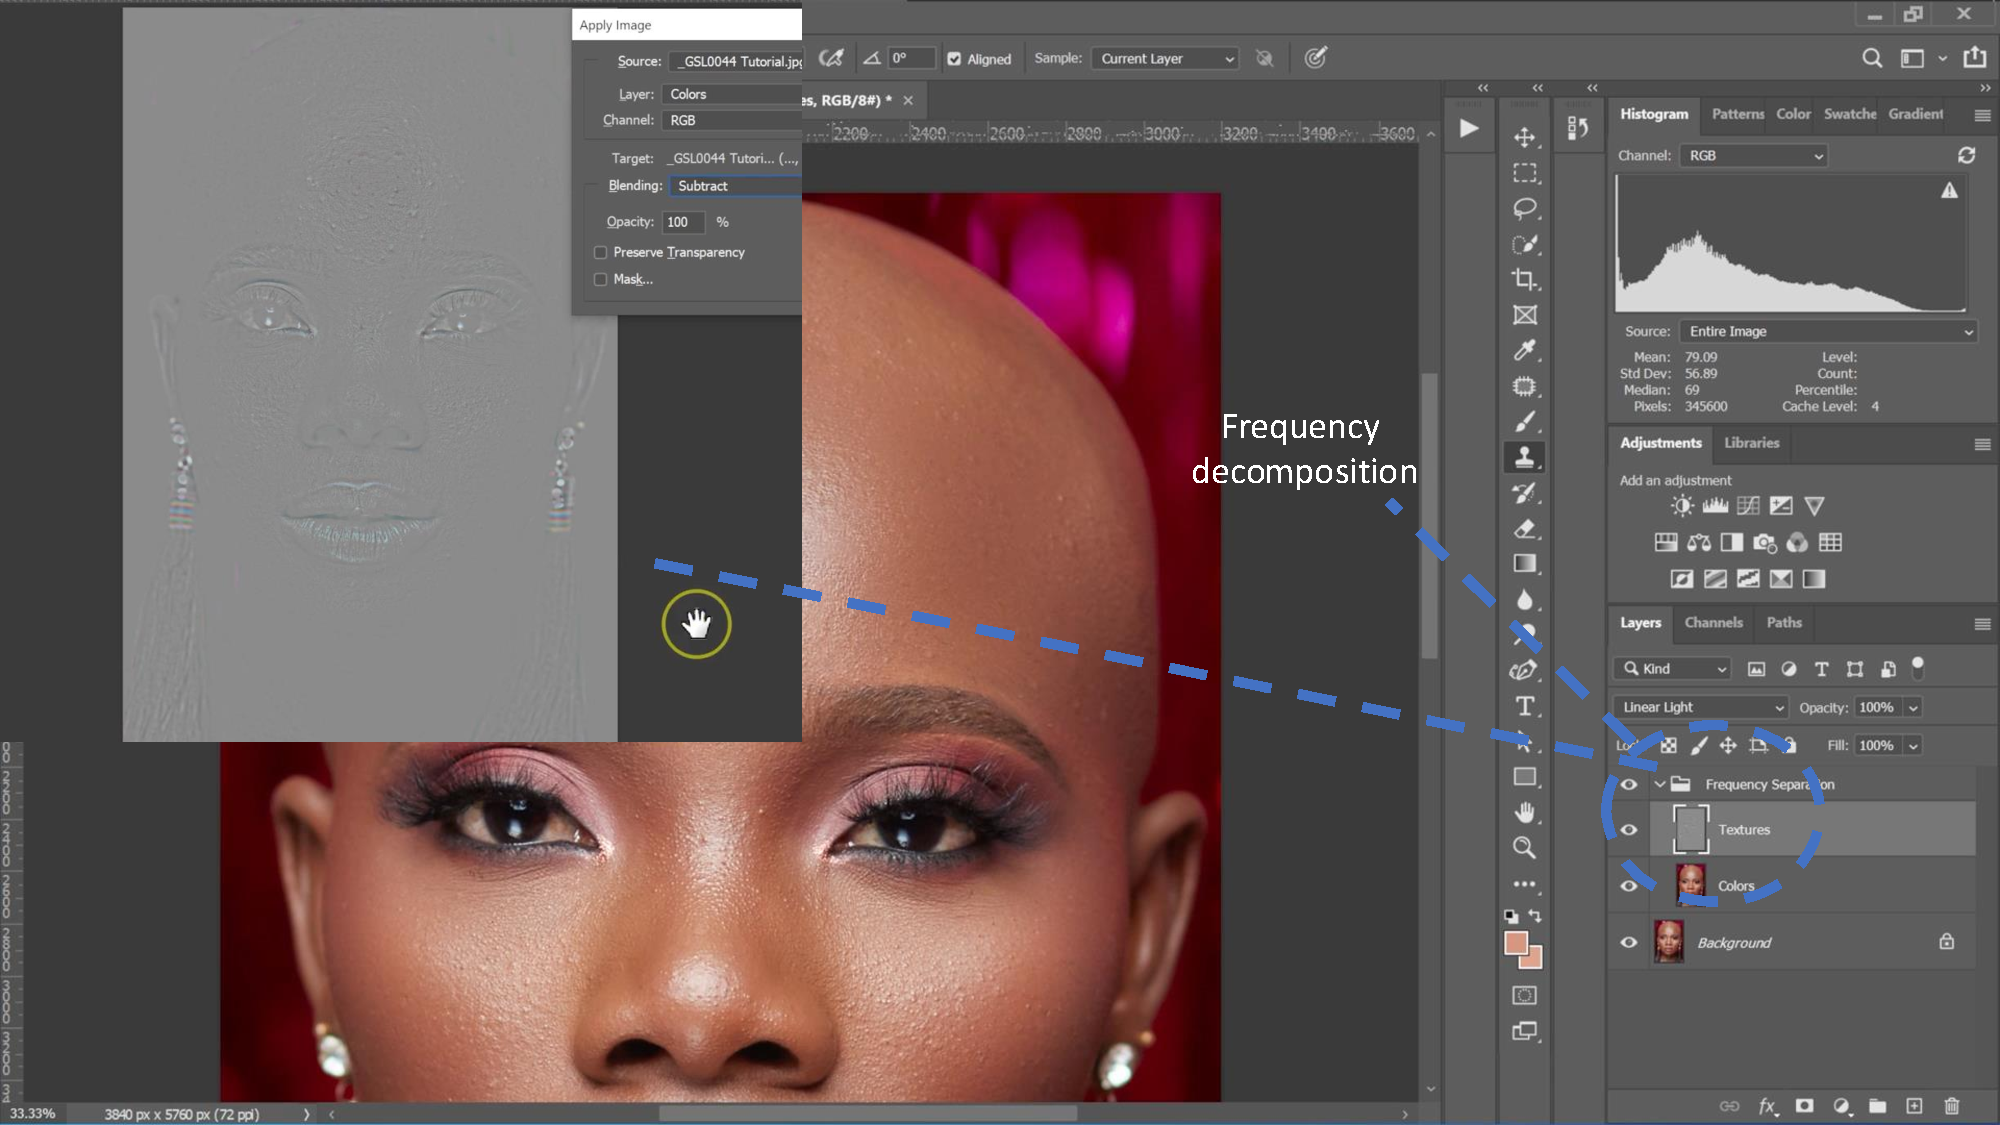
\includegraphics[width=\columnwidth]{Chapters/detail-retouching-figs/PS1.pdf}
    \caption{Frequency decomposition allows artists to have a higher control over different frequency components of an image. Here, the layer shown in the top-left corner is obtained by high-pass filtering of the portrait in the background. Screenshots from [Eustace Kanyanda, 2022].}

\label{fig:PS-high-pass}
\end{figure}

\item Second, image patches of similar content, e.g. skin or hair, are retouched similarly. This means similar patches in the patch space translate into similar edits. The proposed representation leads to a different transformation for patches of differing content. Local filters can offer such edits, where similar contents, such as pores, transform into a similar content, such as a smooth texture:
\begin{figure}[ht]
\centering
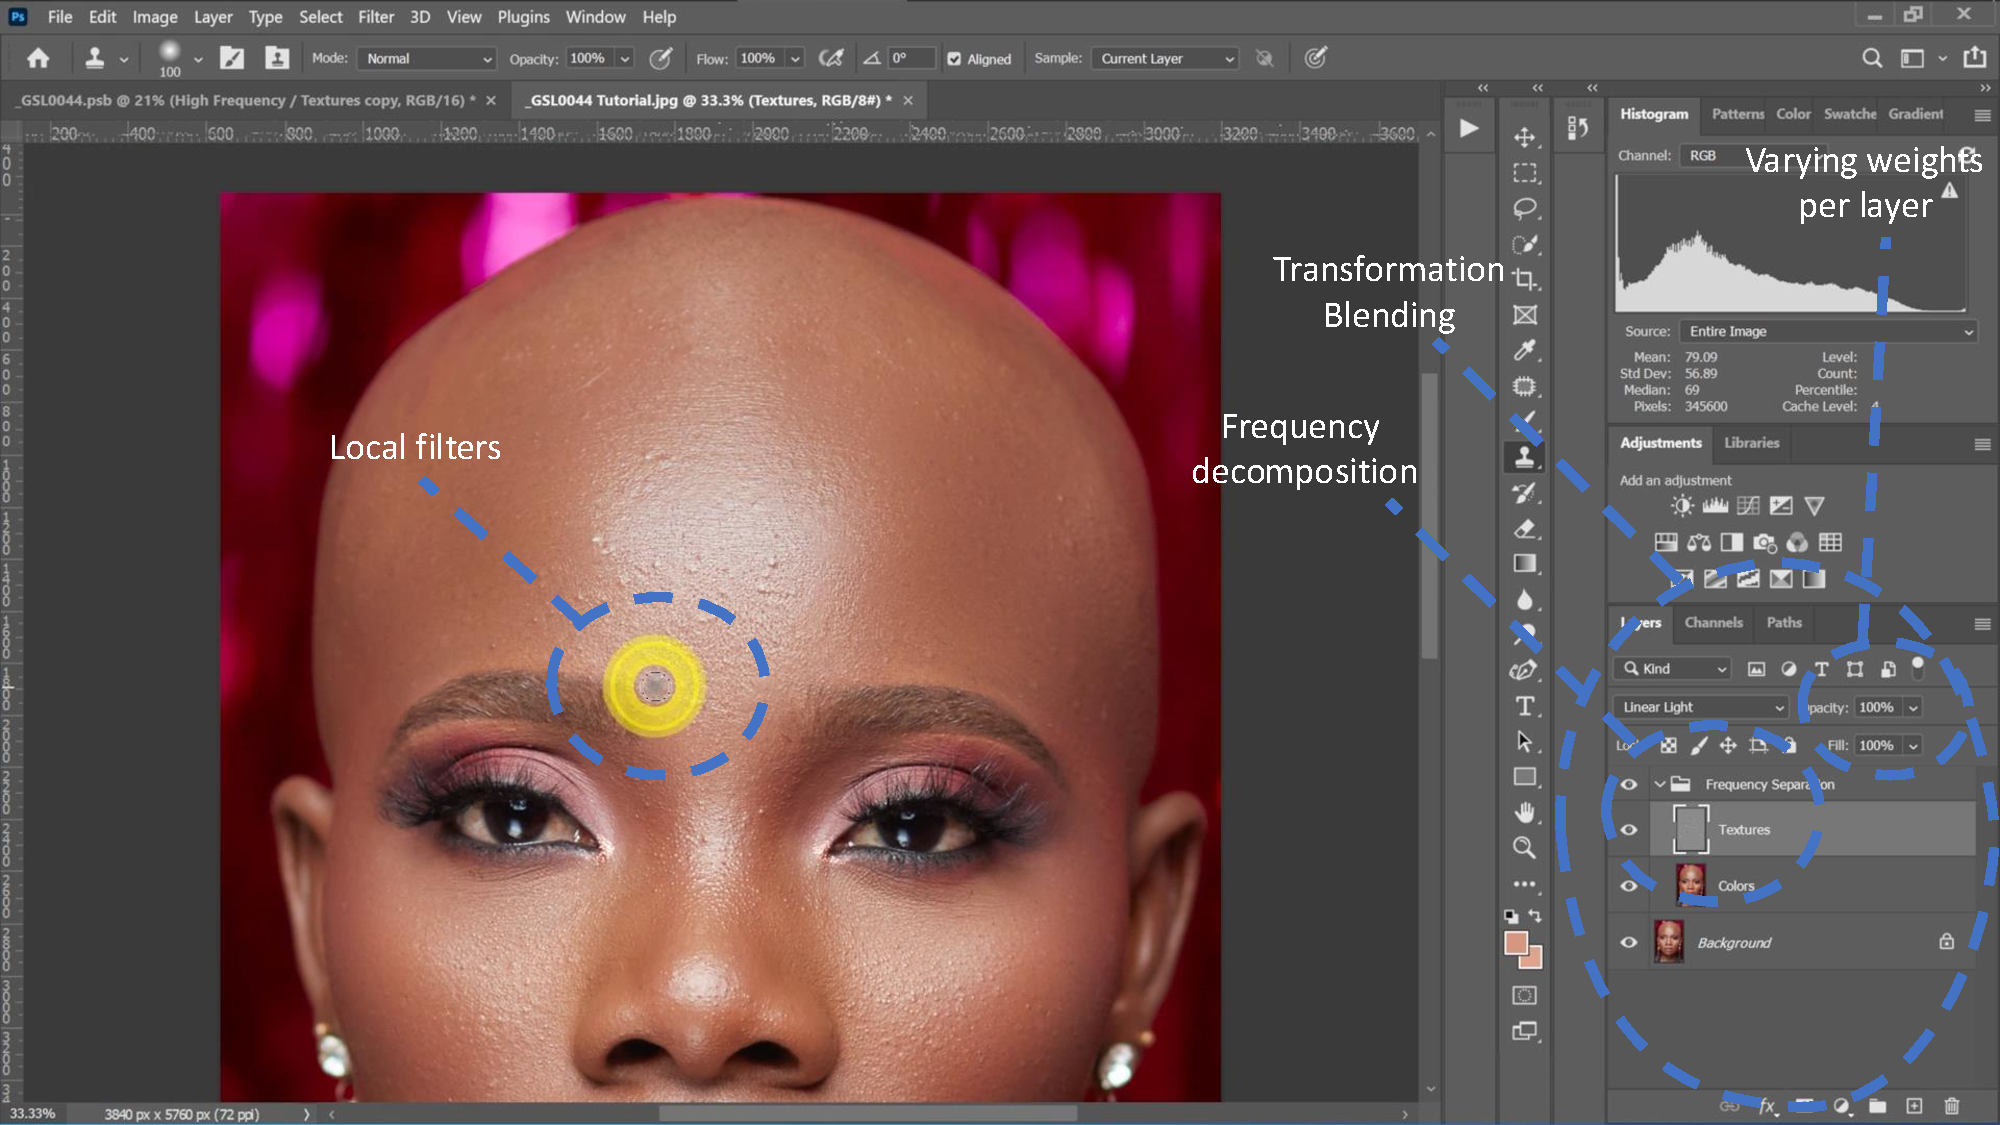
\includegraphics[width=\columnwidth]{Chapters/detail-retouching-figs/PS3.pdf}
    \caption{Local filters, such as brushes, help smoothing the skin by removing the undesired pores on the face. However, it is a tedious task for artists, requiring them to go through each of the visible pores.}

\label{fig:PS-brush}
\end{figure}

\item Third, these edits, global and local adjustments, are typically applied in separate layers and then blended with a subjective opacity value. The neural transformation blending with an MLP block outputting the weights per layer replicates the composition of different layers with their corresponding opacity values:

\begin{figure}[ht]
\centering
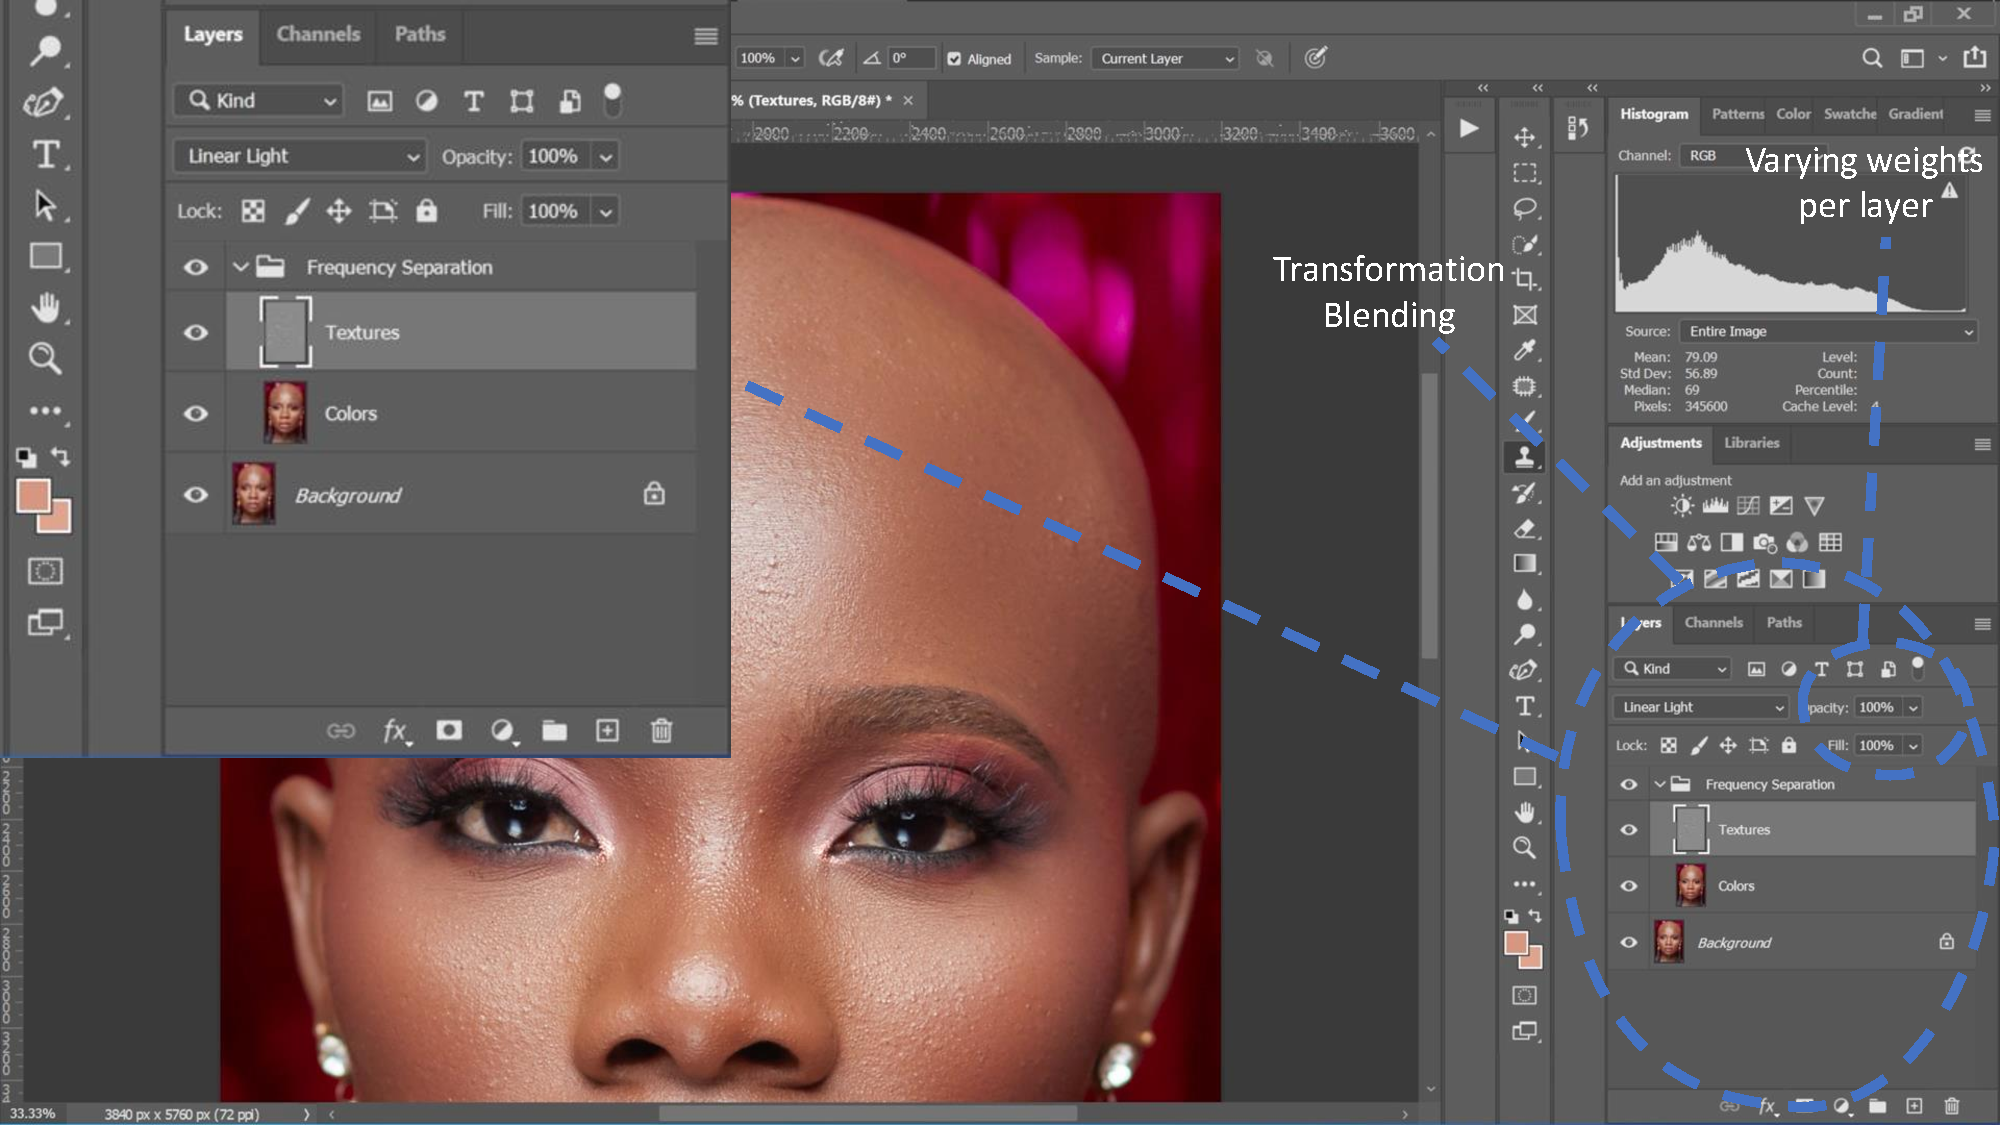
\includegraphics[width=\columnwidth]{Chapters/detail-retouching-figs/PS2.pdf}
    \caption{Artists usually work on separate layers, adjusting varying properties, such as texture, colour, etc. Later, these layers are blended together with their corresponding "opacity" values, shown in the box above the layers.}

\label{fig:PS-all-together}
\end{figure}

\end{itemize}
Although professional artist pipelines inspire this work, I illustrate in the next sections that this new image-to-image mapping representation can replicate the effect of and transfer edits for many filters.



\begin{landscape}\centering
\vspace*{\fill}
\begin{figure}[htpb]
  \centering
  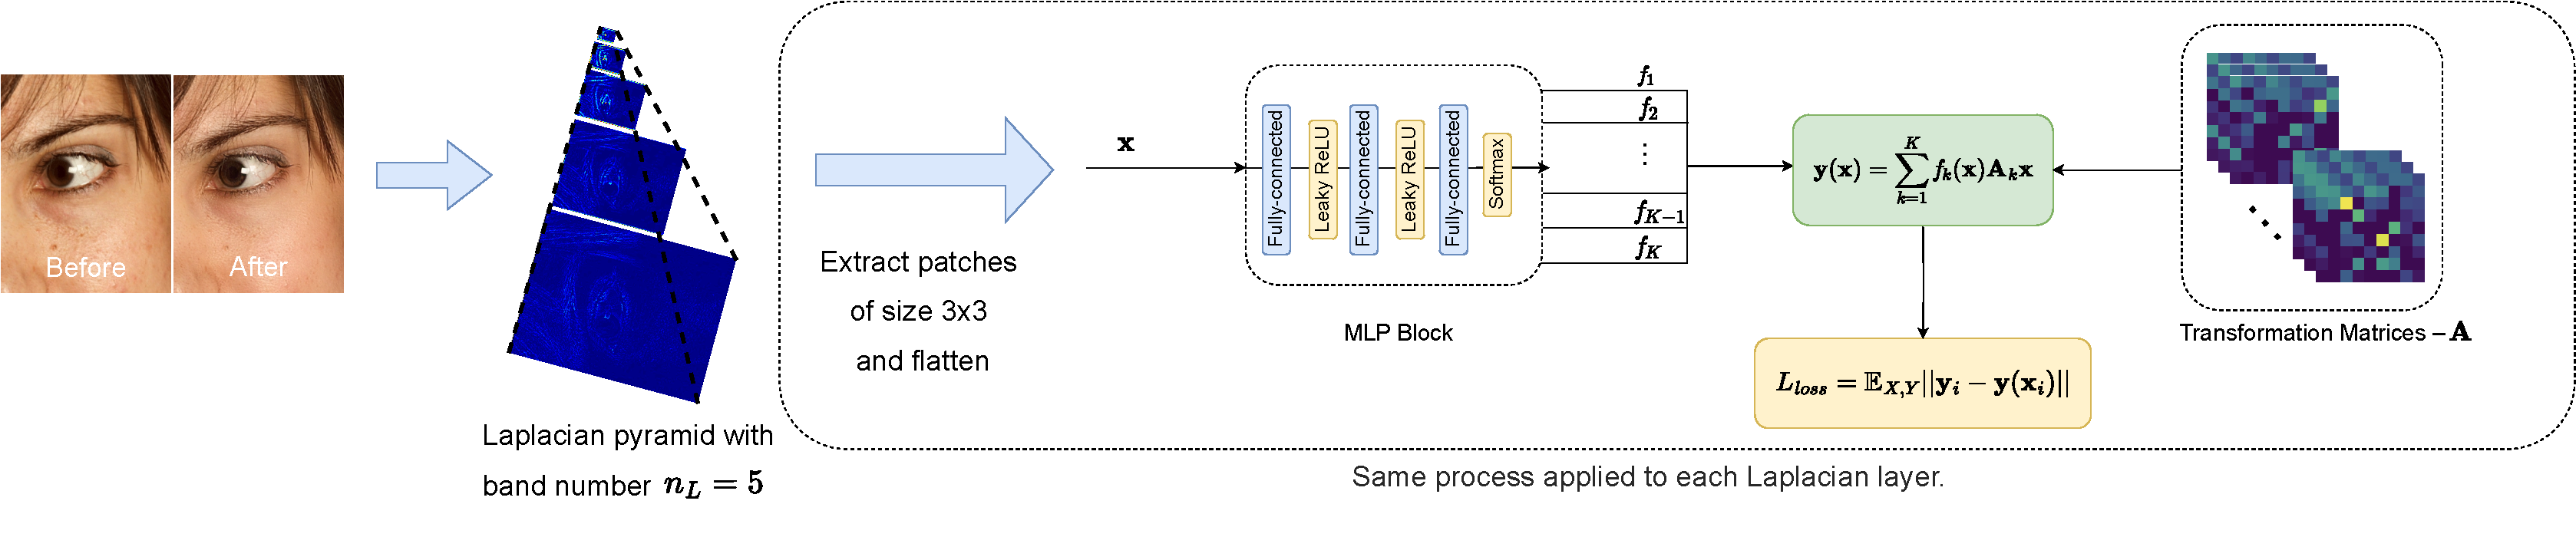
\includegraphics[width=1.5\textwidth]{Chapters/detail-retouching-figs/MainFig.pdf}
  \caption{The proposed technique learns a separate mapping per frequency band by decomposing images into five different bands with a Laplacian pyramid. At each Laplacian band $l$, a separate mapping is defined between flattened patches $\mathbf{x}_i$, $\mathbf{y}_i$ extracted from before-after bands $X_l$, $Y_l$. The field based method (MLP block) adapts transformations to input patches, providing local context-aware adjustments. The transformation matrices and MLP parameters are learned jointly from scratch for each Laplacian band of the before-after pair.}
\end{figure}
\vfill
\end{landscape}


%\begin{landscape}
%\centering
%\begin{figure*}[th] % "[t!]" placement specifier just for this example
%	\centering
%	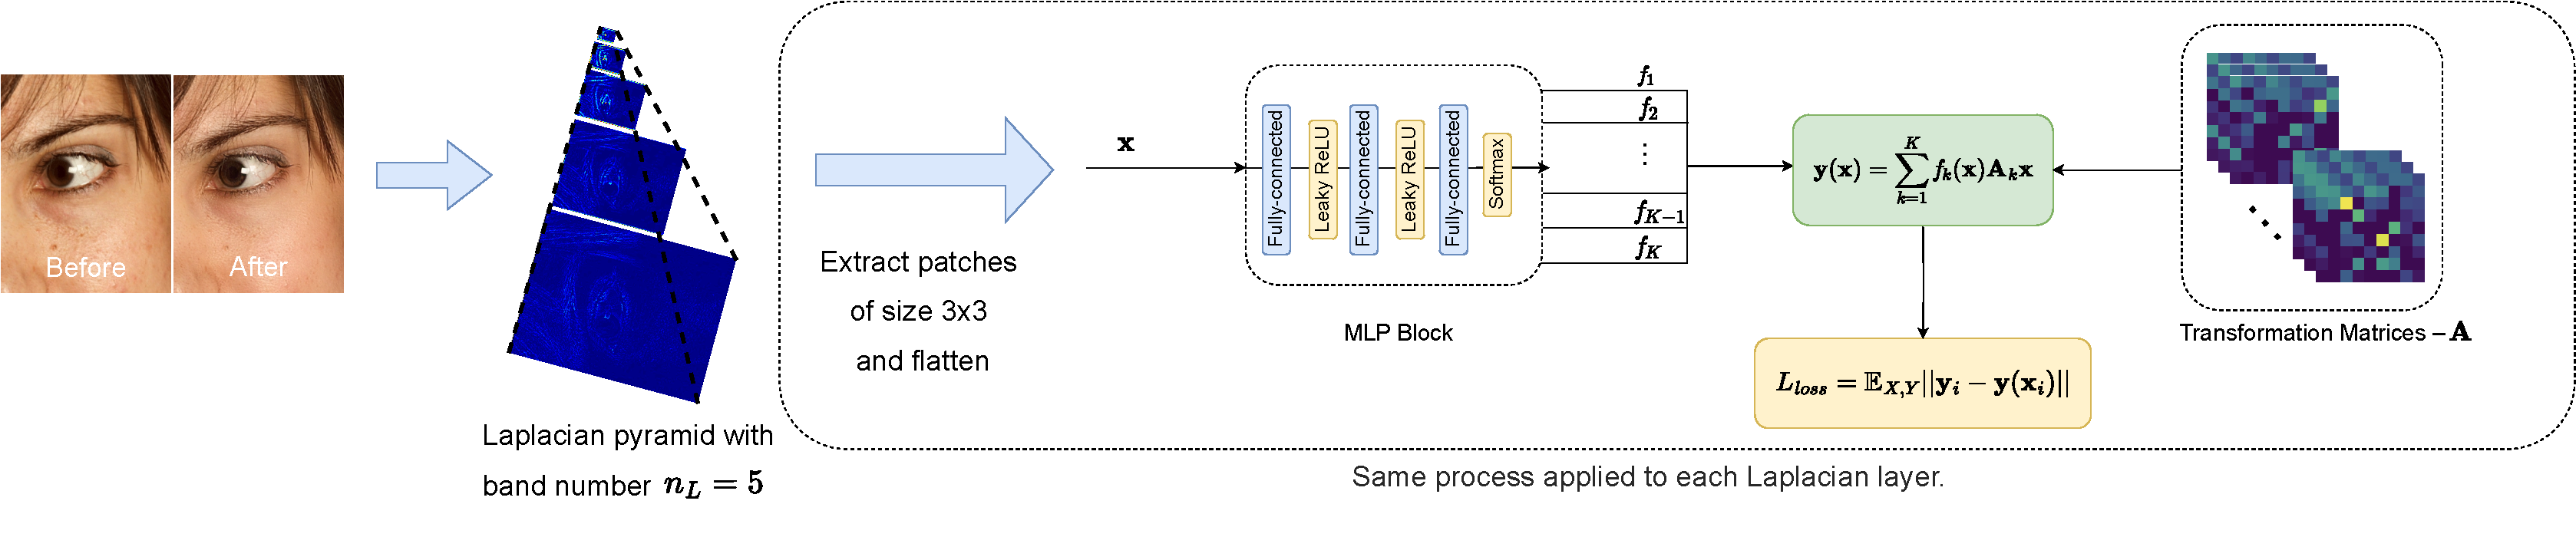
\includegraphics[width=1.5\textwidth]{Chapters/detail-retouching-figs/MainFig.pdf}
    % \includesvg[width=\textwidth]{myfig.svg}
  % \hfill
 %   \caption{The proposed technique learns a separate mapping per frequency band by decomposing images into five different bands with a Laplacian pyramid. At each Laplacian band $l$, a separate mapping is defined between flattened patches $\mathbf{x}_i$, $\mathbf{y}_i$ extracted from before-after bands $X_l$, $Y_l$. The field based method (MLP block) adapts transformations to input patches, providing local context-aware adjustments. The transformation matrices and MLP parameters are learned jointly from scratch for each Laplacian band of the before-after pair.}

%\label{fig:modelT}
%\end{figure*}
% \end{landscape}

\section{One-shot retouching}
\label{sec:Methodology}

\subsection{Frequency decomposition}\label{sec:thePatchMap}
% \myworries{Modify equations in the box - transpose is unnecessary}

I first decompose example and input images into different frequency bands by constructing a Laplacian pyramid to capture details at multiple scales. In principle, it is possible to utilise any multiscale image decomposition method. However, I observed that a basic Laplacian pyramid helped in capturing more accurate and generalisable results compared to a guided or bilateral pyramid. Therefore, I decompose images by

\begin{equation} 
	X_l = L_l(X) = 
 \left \{ \begin{aligned}
        X - G(2) \ast X \hspace{5mm} &l=0\\
        G(2^l) \ast X - G(2^{l+1}) \ast X \hspace{5mm} &l>0,
       \end{aligned}
 \right.
\end{equation}
where $G(\sigma)$ is the normalised Gaussian kernel, and $\ast$ denotes convolution. I also store the low-pass filtered image $S(X)$ such that $X = S(X) + \sum_{l=0}^{n_L} L_l(X)$. I then downsample each $L_l(X)$ and $S(X)$ according to the maximum frequency present at that band. This allows me to use small $3 \times 3$ patches at each band. In the experiments, I used $n_L = 5$ bands for the Laplacian pyramid.


Since each band is processed independently, I explain the steps of our technique below for two generic images $X$ and $Y$.


\subsection{Transformation blending}\label{sec:Blending}

The mapping is defined between patches $\mathbf{x} \in \mathbb{R}^{d_X}$ to $\mathbf{y} \in \mathbb{R}^{d_Y}$ extracted from $X$ and $Y$, respectively, where the patches are denoted by vectors stacking the pixel values, and the patch spaces are defined by $\mathbb{R}^{d_X}$ and  $\mathbb{R}^{d_Y}$. For all results in this work, I work with $3 \times 3$ patches and thus $d_X = d_Y = 9$.

The mapping takes the form of a weighted average of learned transformation matrices $\mathbf{A}$, where each transformation matrix $\mathbf{A}_k$ is first multiplied with its corresponding blending weight: 

\begin{equation} 
	\mathbf{y} (\mathbf{x}) = \sum_{k=1}^K
	\mathit{f}_k (\mathbf{x}) \mathbf{A}_k \mathbf{x},
	\label{eq:weightedSum}
\end{equation} 
Here, $K$ is the number of transformation matrices, and $f_k$ are the blending weights, learned by an MLP block of output size $K$. The $\mathbf{A}_k$'s and $f_k$'s are jointly learned by minimizing the following loss on patches extracted from the before and after images.

\begin{equation}
    L_{loss}  = \mathbb{E}_{X, Y} || \mathbf{y}_i -   \mathbf{y} (\mathbf{x}_i) ||
\end{equation}

Each $\mathbf{A}_k$ corresponds to a different type of transformation and the $f_k(\mathbf{x})$'s, represented with the MLP, allow for a smooth transition between different transformations. The form of $f_k$'s is relatively simple with three fully-connected layers and nonlinear activation functions applied after each layer. This blending forms a simple but expressive transformation as illustrated in Section \ref{sec:results}.

\subsection{Retouching an input image}

I process the input image $I$ the same way as the before-after pair. First, I decompose the input into its Laplacian layers and then extract patches for each layer. After applying the learned mappings $M_l$ to the patches of the corresponding layers $L_{l}(I)$ independently, I then reconstruct the Laplacian bands of the output image $O_l$ by placing the patches in their spatial locations and averaging over the overlapping regions. Later, I obtain the final output image $O$ by summing the outputs $O_l$ and the residual of the input image:
\begin{equation}
    O = S(I) + \sum_{l=0}^{n_L} M_l(L_l(I))\,.
\end{equation}




\subsection{Implementation}
\label{sec:Implementation}

\paragraph{Patch size and stride.} In order to capture each frequency band at the right level of detail, I do not upsample the images $L_l(X)$ and use a small $3 \times 3$ patch size (with stride $1$). I experimented with larger patch sizes. However, this turned out to be counterproductive for the detail levelItarget, as details are blurred in larger patches. They also led to overfitting and were, in general, harder to optimise for. I used a stride of $1$, and hence patches overlap on the image plane. The overlapping patches are averaged while reconstructing the image.

\paragraph{Detail and colour modifications.} This work aims to capture intricate details present in highly detailed retouches and a wide range of image processing operators. Based on the observation that various operators can edit materials in the image space using the luminance component~\cite{Boyadzhiev15Band}, I focus on learning changes in luminance while preserving the input chrominance channels. 

\paragraph{Evaluation metrics.} To quantitatively compare the technique with state-of-the-art methods, I used PSNR and SSIM metrics. This is only possible if the before-after image pair was processed with a known, reproducible operator (see Section~\ref{sec:Comparisons} for details).


\paragraph{Training details.}\label{train_det} I train different mappings with the same structure, defined in Equation \ref{eq:weightedSum}, for each frequency band of the Laplacian pyramid. Each mapping consists of one MLP block and $K$ number of transformation matrices, which are learned jointly per frequency band from scratch for each before-after pair. The MLP block employed in the experiments consists of three fully-connected layers and non-linearities applied after each layer. The output size of the last layer is the same as the number of transformation matrices.

To normalize the weights, I choose the last activation function to be Softmax, while for the first two layers, I apply Leaky ReLU. Each transformation matrix is randomly initialised with the uniform distribution in the range of $[0, 1]$. All experiments use the Adam optimiser with a learning rate of $10^{-2}$, which exponentially decays with a decay rate of $0.96$. I use $l_1$ loss function in all experiments. Through backpropagation, both the MLP parameters and the entries of the transformation matrices are jointly learned. The pseudocode for both the training and inference procedures are the following:

\begin{algorithm}
\caption{One-shot Detail Retouching}
\SetKwFunction{FDetailRetouch}{Train}
\SetKwFunction{FPyramid}{LaplacianPyramid}
\SetKwFunction{FMLPBLOCK}{MLPBlock}
\SetKwFunction{FPatch}{ExtractPatch}
\SetKwFunction{Fprob}{Backpropagate}
\SetKwProg{Fn}{Function}{:}{}
\Fn{\FDetailRetouch{'before' image $X$, 'after' image $Y$}}{
	\Comment{Decompose images into its Laplacian bands.}\\
        $X_l \gets \FPyramid(X)$\;
        $Y_l \gets \FPyramid(Y)$\;
        
        \For{$l \gets 0$ \KwTo $n_l$}{
        \Comment{Extract patches from the images.}\\
        $x_i \gets \FPatch(X_l)$\;
        $y_i \gets \FPatch(Y_l)$\;
        $f_k \gets \FMLPBLOCK(x_i)$\;
        $y(x_i) \gets \sum^{K}_{k = 0} f_k(x_i) A_k x_i$\;
        $\mathcal{L} \gets E_{X, Y} \abs{(y(x_i) - y_i)}$\;  
        $(f_k, A_k) \gets \Fprob(\mathcal{L})$}
        }
\end{algorithm}

\begin{algorithm}
\caption{One-shot Detail Retouching}
\SetKwFunction{FDetailRetouch}{Inference}
\SetKwFunction{FPyramid}{LaplacianPyramid}
\SetKwFunction{FMLPBLOCK}{MLPBlock}
\SetKwFunction{FPatch}{ExtractPatch}
\SetKwFunction{Fpatchmerge}{MergePatch}
\SetKwProg{Fn}{Function}{:}{}
\Fn{\FDetailRetouch{input image $I$, blending weights $f_k$, transformation matrices $A_k$}}{

        $I_l \gets \FPyramid(I)$\;
        
        \For{$l \gets 0$ \KwTo $n_l$}{
        $i_i \gets \FPatch(I_l)$\;
        \Comment{Transform input patches $i_i$ with learned weights and matrices.}\\
        $o_i \gets \sum^{K}_{k = 1} f_k(i_i) A_k i_i$\;
        	\Comment{Place the patches on the output grid $O_l$.}\\
        $O_l \gets \Fpatchmerge(o_i)$}
     
        \Comment{Sum all output bands with input residual.}\\
        $O = I_{n_l} + \sum_l O_l$\;
        \Return $O$}
        
\end{algorithm}

\section{Results}
\label{sec:results}


\subsection{Ablation Studies}\label{ablation}
The success of the learned mappings relies on two key components: patch-adaptive retouching and transformation blending. I thus conduct experiments to illustrate the significance of these.

%Ifirst investigate the effect of the number of transformation matrices, $K$. 
% \paragraph*{Transformation Matrices.}
\paragraph{Transformation Matrices.} I compared transformation matrices of size $9 \times 9$ with scalar values. The method still remained spatially-varying, since I left the MLP the same, and used $K=256$ scalar weights. I tested both methods on 100 images and computed average PSNR values. I observed that the technique with matrices performed better than scalar values even in simple algorithmic filters, such as Gaussian and Unsharping Masking (around 2 dB and 3 dB higher PSNRs, respectively). 

As the complexity of a retouching style depends on multiple factors, such as artists’ design choices, user preferences, or the artist toolbox, it is challenging to analyse such effects on retouching examples quantitatively. For simple algorithmic filters, such as a Gaussian filter or unsharp masking, $K=1$ can sufficiently reproduce the filter. In contrast, more complex algorithms, such as a bilateral filter, require more matrices to capture the algorithmic edits accurately (Figure \ref{fig:ablation_K}). Since retouching edits combine the effect of multiple operators and are highly non-linear, I empirically found $K=256$ offers effective results for the retouching examples. 

\begin{figure}[th] % "[t!]" placement specifier just for this example
    \centering
	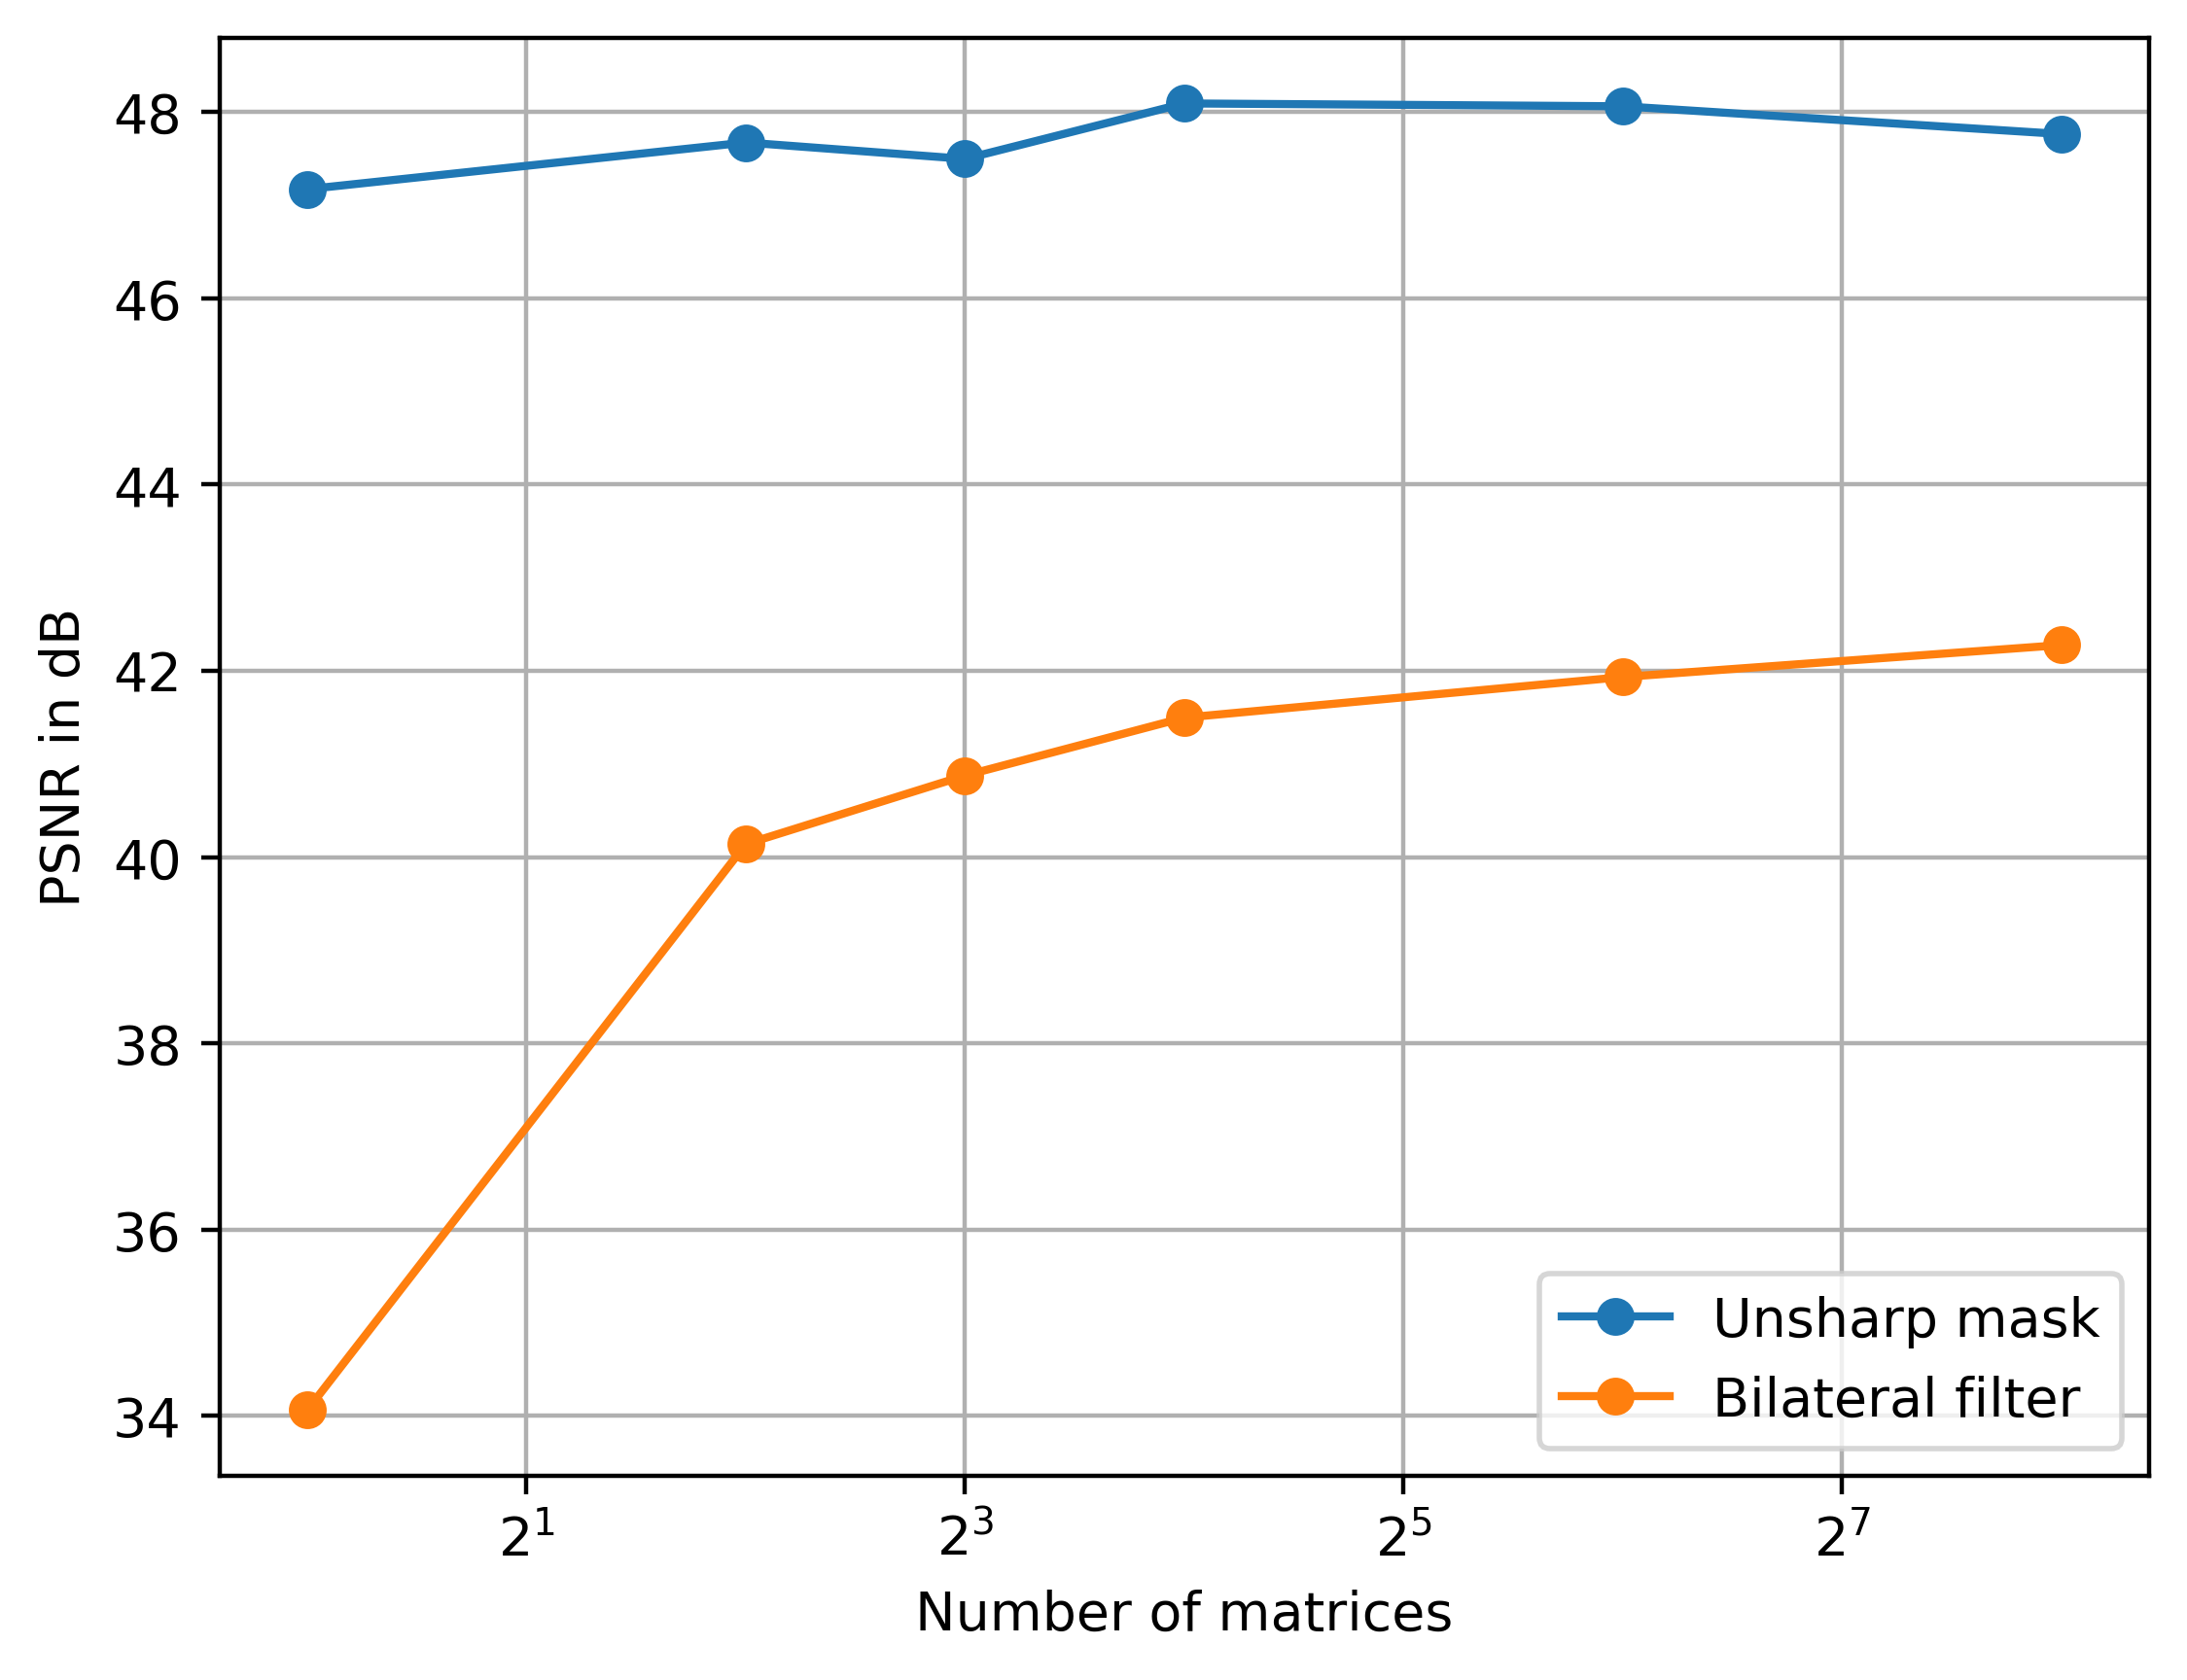
\includegraphics[width=0.5\columnwidth]{Chapters/detail-retouching-figs/ablation_matrices.png}

    \caption{The higher the complexity of the learned algorithm, the more transformation matrices the technique requires to capture the effects on local regions accurately. While $K=1$ can be sufficient for the model to capture unsharp masking, it requires more matrices to represent bilateral filtering precisely.}

    \label{fig:ablation_K}
\end{figure}

\begin{figure}%[H]
\centering
\includegraphics[width=0.8\columnwidth]{Chapters/detail-retouching-figs/AblationStudy_K.pdf}
    \caption{An MLP regressor cannot capture local edits, resulting in inaccurate retouching edits, such as blurring on the skin or around the eyes.}

\label{fig:ablation_MLP}
\end{figure}
% \paragraph*{Patch-adaptive Transformation Blending.}
\paragraph{Patch-adaptive Transformation Blending.} I also compared the patch-adaptive mapping to an MLP regressor on the extracted patches. This directly learns the mapping from the decomposition of example before-after images instead of utilising blended transformations. The MLP regressor follows a similar architecture as the MLP block (Figure \ref{fig:modelT}), with the only difference being the last activation function. I used Leaky ReLU here, since the Softmax function outputs pseudo-probabilities and is unsuitable for regression. Not explicitly handling the spatially-varying structure of the mapping and directly regressing limits the expressiveness of the model. This results in blurry results as shown in Figure~\ref{fig:ablation_MLP} because such a model cannot capture edits in intricate details, such as highlights around eyes and hair or brightening of the skin. I also tried increasing the capacity of the MLP regressor but did not observe much improvement in performance.


\paragraph{Weights visualisation.} To study the effectiveness of the weights across an image, I randomly chose eight transformation matrices and reconstructed their corresponding weights per Laplacian band. The reconstruction occurs in the same way as image patches, being placed in their location. However, since each patch of size $3 x 3$ has only one weight,Ido not need to take average over overlapping areas. Also, cropped the last eight columns of the reconstructed weight images since they were all zeros due to the size difference with patches. Figure \ref{fig:weight-vis} shows eight different reconstructed weights for each Laplacian band, obtained by the model trained with the example images in the teaser (middle \& right insets). The input to the model and the output retouched image are shown on top. As can be seen, the weights have varying values around different regions across the bands. Note that the resolution of the bands is increased to the same size for better visualisation. Otherwise, during training, each band’s resolution is kept its size based on the Laplacian pyramid.

\begin{figure}%[H]
\centering
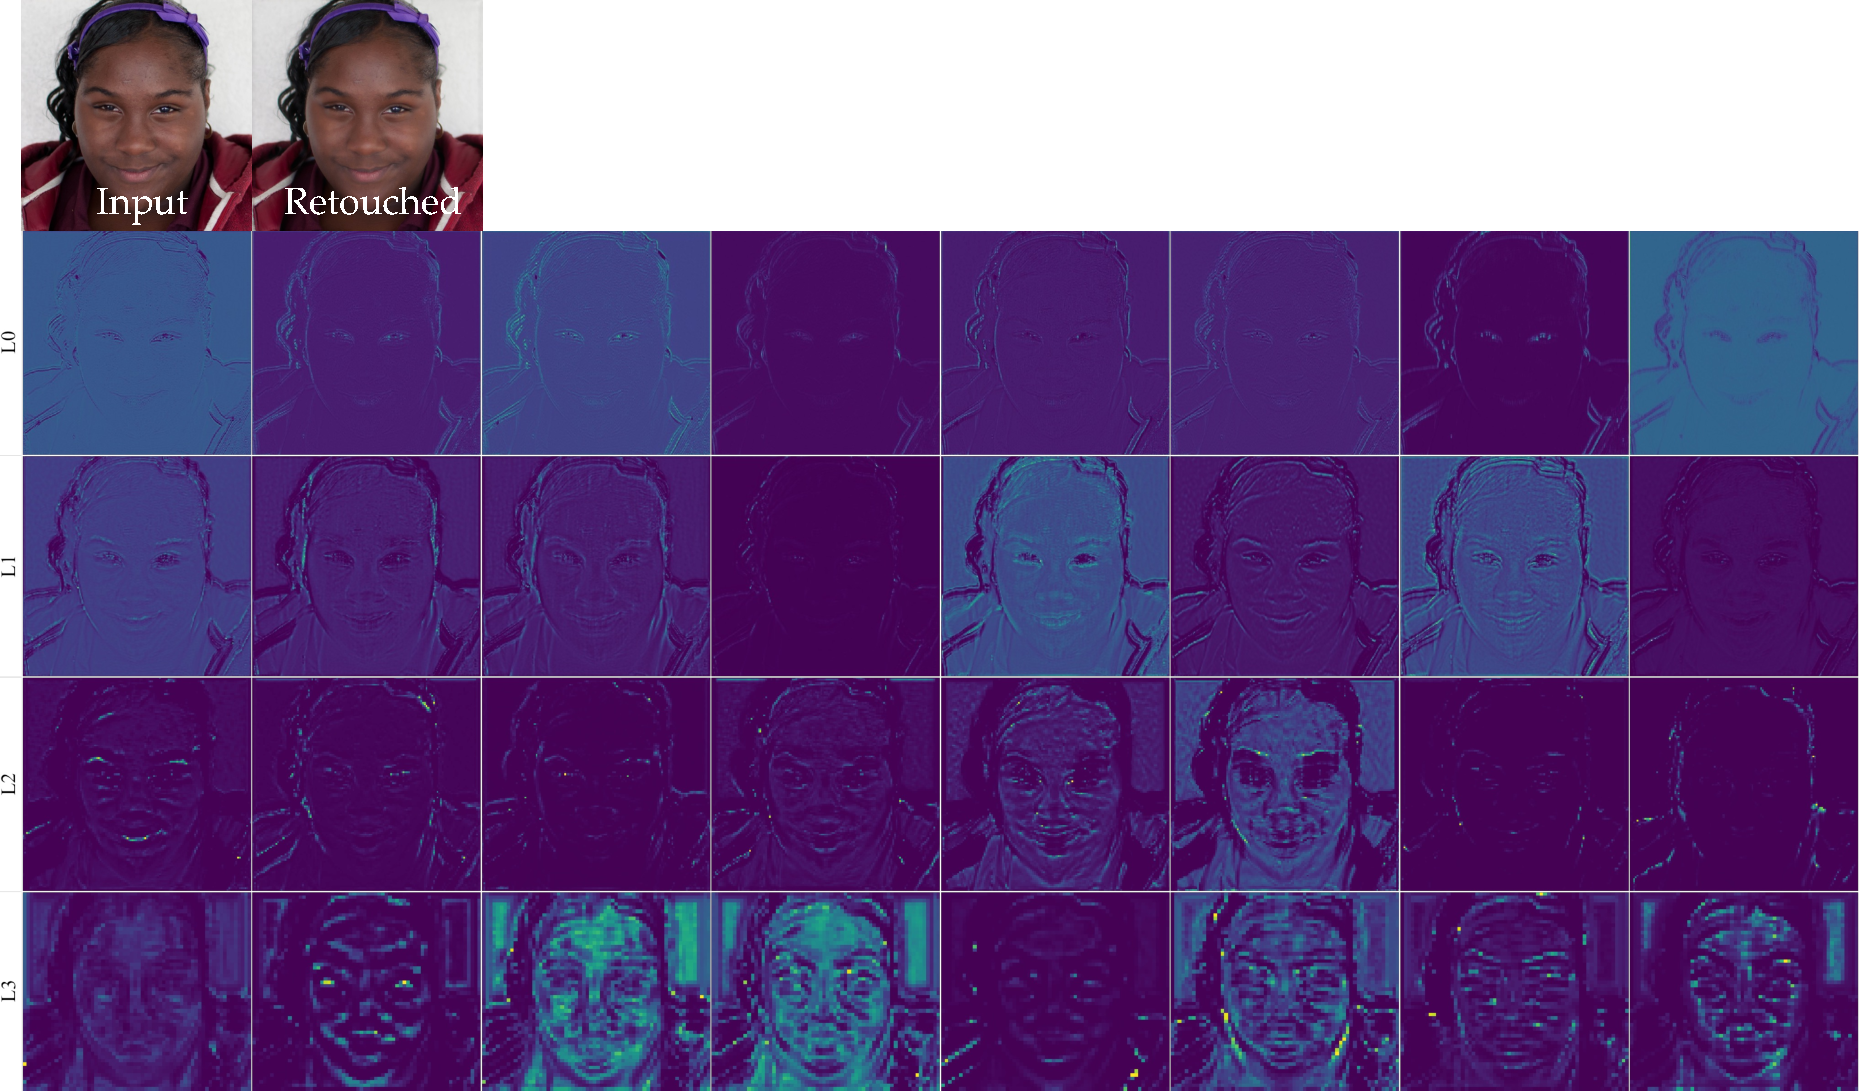
\includegraphics[width=0.8\columnwidth]{Chapters/detail-retouching-figs/weight_visualise.pdf}
    \caption{Visualisation of the reconstructed patch-adaptive weights of the model trained with example images in the teaser. Here, the input to the model is shown on top, and each row shows the weights in the corresponding Laplacian band, indicated on the left.}

\label{fig:weight-vis}
\end{figure}

\subsection{Qualitative Results}
I tested the proposed technique on a diverse range of before-after pairs, including face images from the \textbf{FFHQ} dataset \cite{karras2019style}.I focus on human portraits and face retouching in the experiments as they are arguably the most common and prioritised types of photos for retouching.I also illustrate that the technique provides visually pleasing results in different types of images, such as materials or rooms, and accurately captures image processing filters.

\begin{figure}[th] % "[t!]" placement specifier just for this example
    \centering
	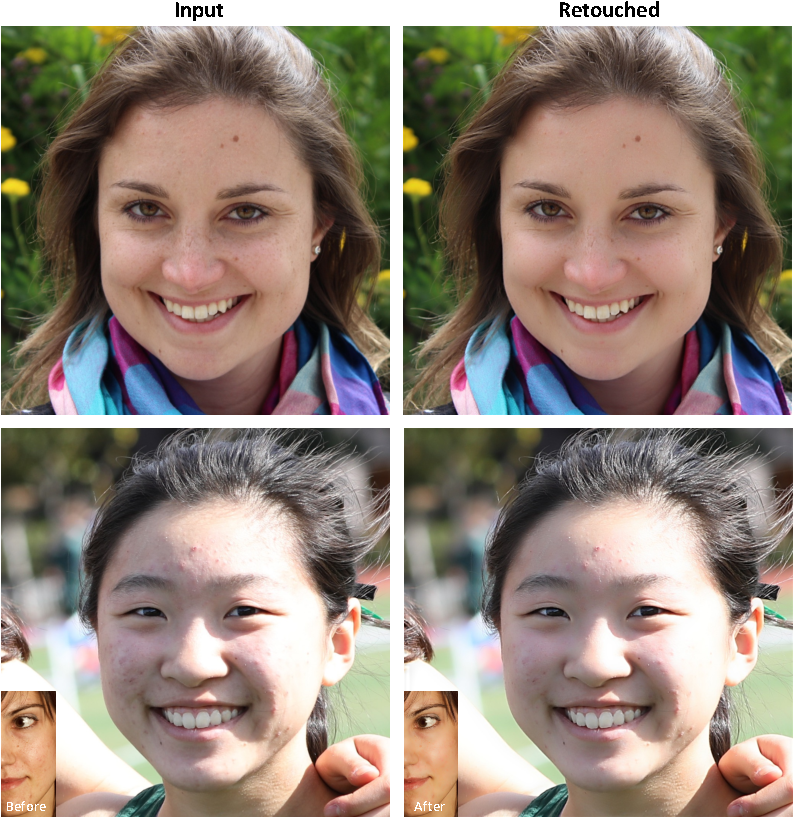
\includegraphics[width=0.8\columnwidth]{Chapters/detail-retouching-figs/res_diff_light_2_cvmp.pdf}
    \caption{\label{fig:newdataset_ex}The reproduced retouching style from the example pair (inset) improves skin texture without affecting fine details, such as eyes and hair, for a visually improved portrait. Moreover, the technique generalises well to faces with different lighting conditions and accurately reproduces the example retouching style.}
 
\end{figure}
% \paragraph*{Face retouching - skin and eye filters:}\label{faceretouching}
Human faces pose a particular challenge for the one-shot setting. However, the model can still capture highly nonlinear retouching edits and generalises well to different types of faces, view directions, and lighting conditions, as illustrated in Figures~\ref{fig:teaser}, ~\ref{fig:newdataset_ex}, and ~\ref{fig:retouchingstyles}.

\begin{figure}[th] % "[t!]" placement specifier just for this example
	\centering
	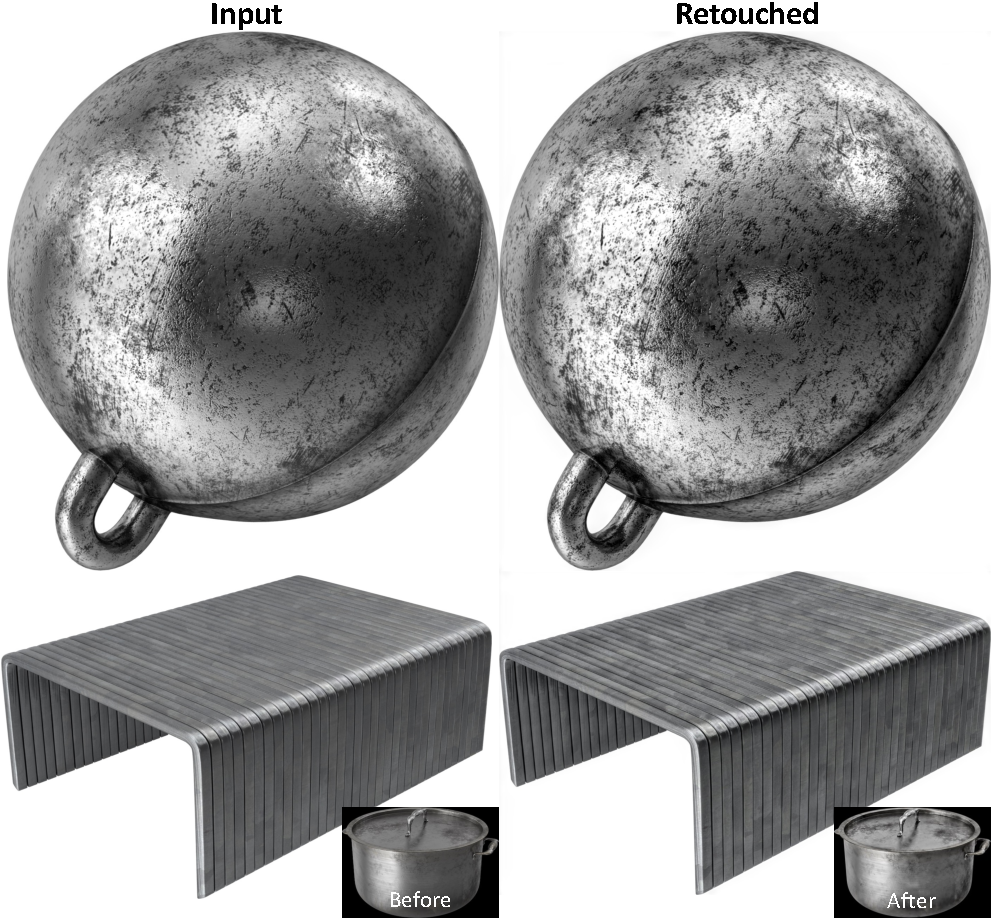
\includegraphics[width=0.8\columnwidth]{Chapters/detail-retouching-figs/MaterialResults.pdf}
    \caption{\label{fig:material_res}Material editing results on photos (left), and rendered images (right), based on the before-after pair (inset). The details, such as scratches or lines are emphasised, and materials became shinier. Image courtesy of royalmix (top and bottom-inset), tsmdunn (bottom). (PixelSquid).}

\end{figure}

The example pairs in Figures~\ref{fig:teaser}, ~\ref{fig:newdataset_ex}  and ~\ref{fig:retouchingstyles} were generated by brushing onto the skin with artist created brushes, eye sharpening (sharpening example in Figure~\ref{fig:teaser}), and further brightness/contrast adjustments. These brushes first decompose the skin into a detail and base layer, typically with frequency decomposition, alter the detail layer and blend it with the base layer. They differ in how (1) they decompose the skin into the layers, i.e., what frequencies are in each layer, and (2) they edit and blend each layer with different opacity values. This variation creates retouching nuances, as shown in Figure~\ref{fig:retouchingstyles}. The framework can still accurately capture such slight differences in styles. 

\begin{figure}[th] % "[t!]" placement specifier just for this example
    \centering
	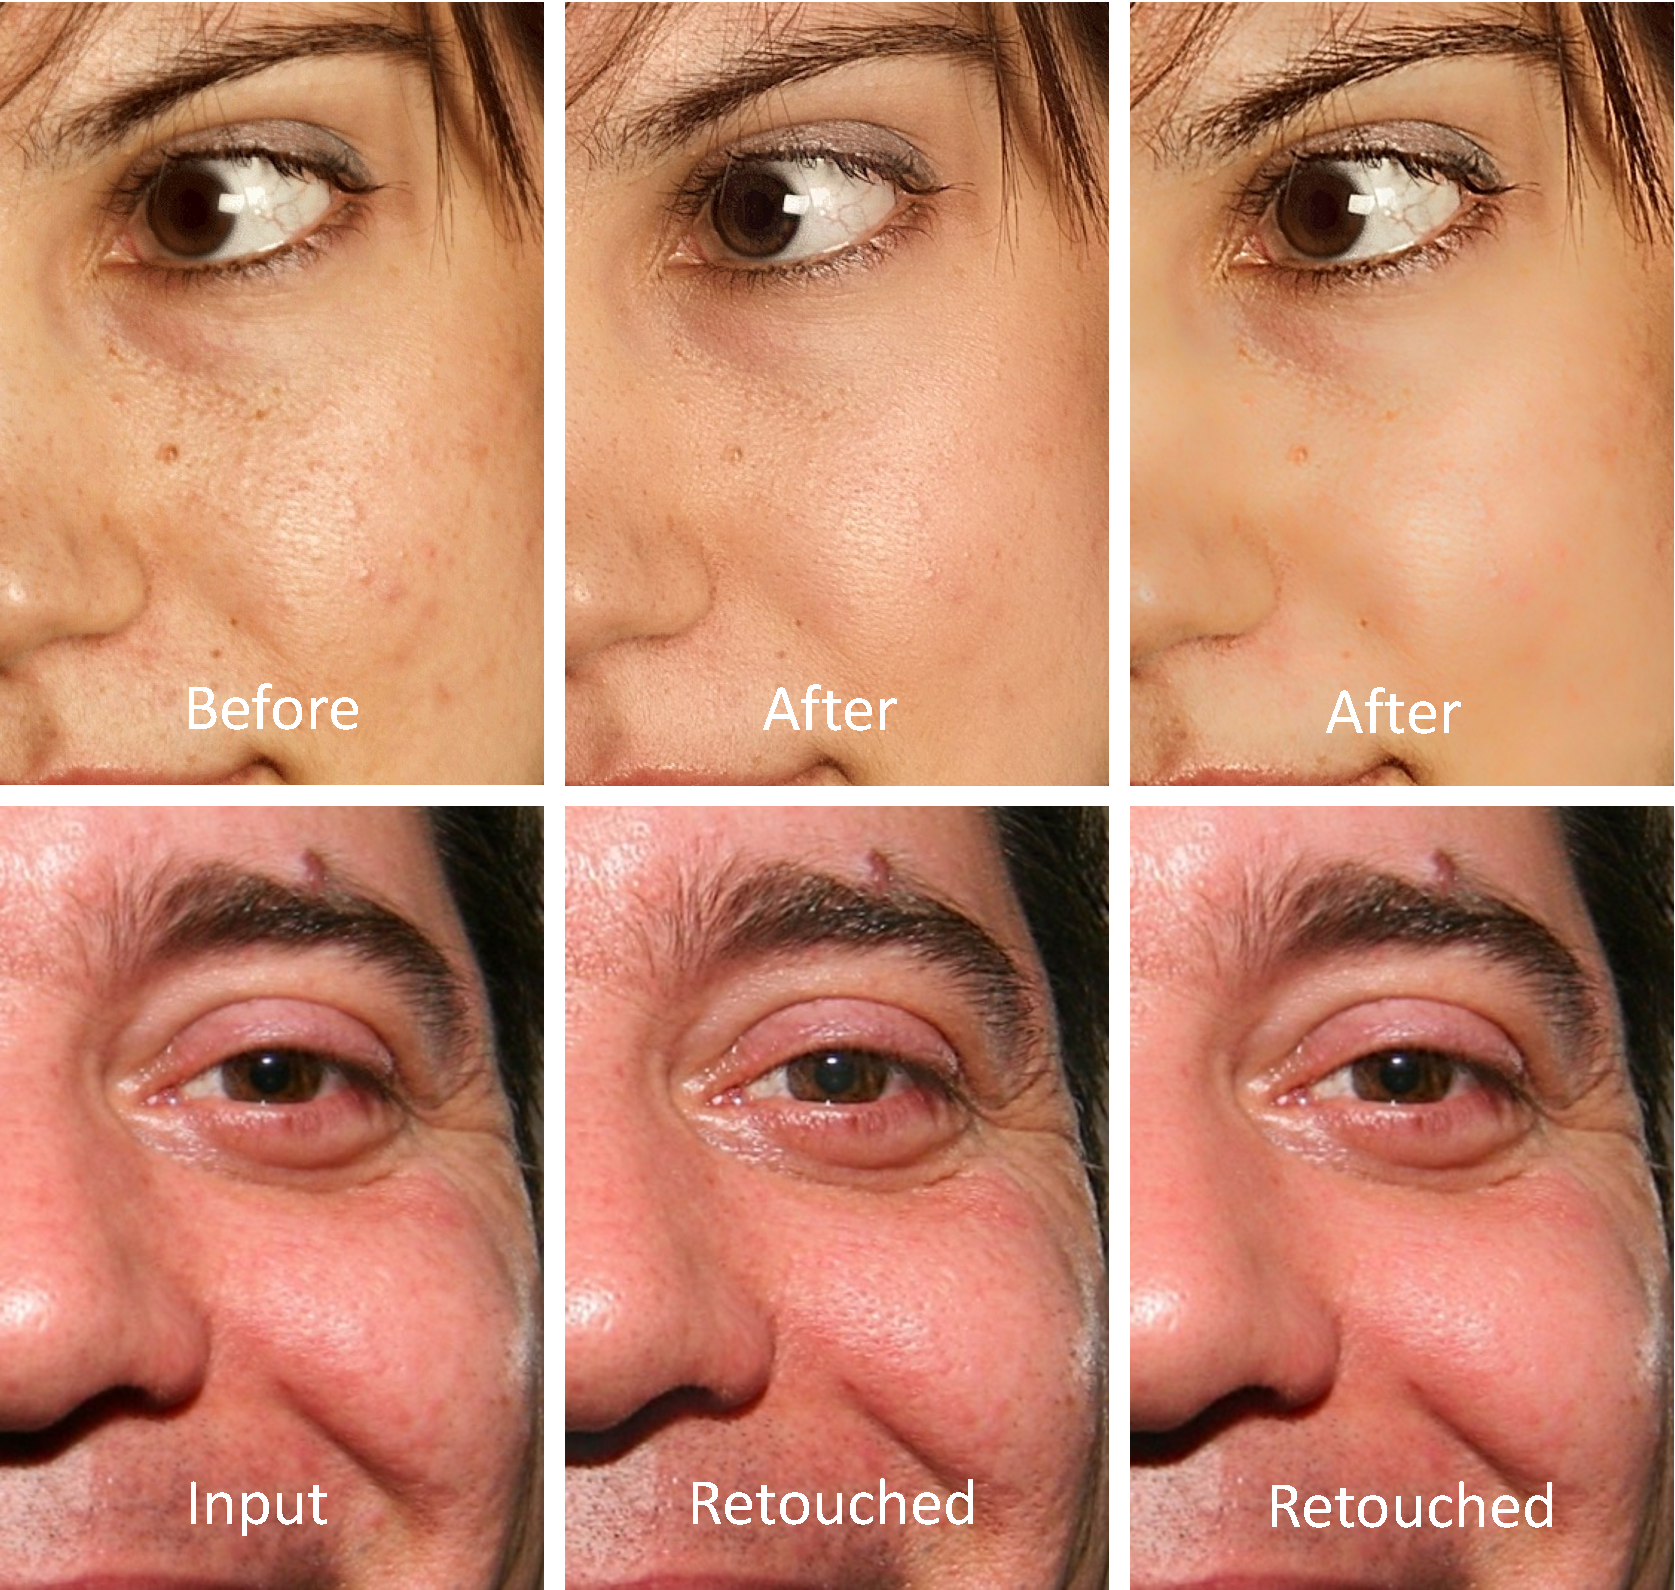
\includegraphics[width=0.8\columnwidth]{Chapters/detail-retouching-figs/Nuances.pdf}
  % \hfill
    \caption{Our patch-adaptive technique can accurately capture the nuances between different
    retouching styles as given by the examples (top row).}
\label{fig:retouchingstyles}
\end{figure}

In all experiments, intricate details of the desired retouching, such as small-scale texture, eye, facial hair or material details, and global features, such as overall lighting and tone, are accurately reproduced. It is interesting to observe that the \emph{glamour} implied by, e.g., the example retouching in Figure~\ref{fig:newdataset_ex} is transferred from the example pair very accurately without causing an artificial look. Zooming into the skin reveals that pores and wrinkles are minimised, and the blemishes and discolouring of the skin are eliminated. At the same time, depending on the retouching edit, details, such as eyes or material texture, are more highlighted or preserved, and delicate features such as hair are preserved well (Figures ~\ref{fig:newdataset_ex}, ~\ref{fig:material_res} and ~\ref{fig:retouchingstyles}). 


In summary, the proposed technique efficiently edits such intricate details, due to the significantly distinct local statistics of the texture at multiple scales, without affecting overlaying structures thanks to its spatially-varying nature and frequency decomposition. 

\subsection{Comparison with the state-of-the-art}
\label{sec:Comparisons}


Although there are various works related to automatic photo enhancement, to the best of our knowledge, none of them works with a single example pair for detail retouching. Therefore, I compare the results with closely related automatic image-to-image translation methods, namely U-Net \cite{ronneberger2015u}, ASAPNet generator \cite{shaham2021spatially}, and Deep edge-aware filters \cite{xu2015deep}. 

I trained each network from scratch with one \textit{before-after} pair. To train the U-Net architecture, I changed the activation function of its last layer to ReLU and used $l_1$ loss function with Adam optimiser (same as ours). Similar to the proposed method, ASAPNet is also a spatially-adaptive network. However, it is instead designed to hallucinate new details. Therefore, I trained their generator model in a similar fashion with $l1$ loss, removing the discriminator. After observing that bilinear downsampling in their model causes checkerboard artifacts, I removed this operator and learned an MLP per pixel, which caused the model to be highly complex with too many parameters. 


\begin{table*}[th]
\centering
\caption{Quantitative performance comparison for the reproduction of various image processing filters. Average PSNR and SSIM values are computed over 182 images of different types of images including faces, landscapes, materials, and rooms. Qualitative results can be found in the supplementary material.We highlight \colorbox{blue!25}{best PSNR} and \colorbox{orange!25}{best SSIM} results.}


\resizebox{\textwidth}{!}{\begin{tabular}{l@{\hskip 0.2in}c@{\hskip 0.1in}c@{\hskip 0.1in}c@{\hskip 0.1in}@{\hskip 0.1in}c@{\hskip 0.1in}c@{\hskip 0.1in}c}
    % \begin{tabular}{@{}cccccc@{}}
    \toprule
     \multicolumn{5}{c}{{Comparison results (PSNR in dB / SSIM)}} \\ \cline{1-5}
     {Filter Type} & {ASAPNet Generator} & {Deep Edge-aware} & {UNet} & {Ours}\\
     \midrule
    Gaussian & \cellcolor{orange!25}{39.36 / 0.983} & 36.52 / 0.979 & 40.52 / 0.979 & \cellcolor{blue!25}{40.67 / 0.983} \\%\midrule
    %   \hline
     Unsharp Mask & 29.77 / 0.889 & 32.62 / \cellcolor{orange!25}{0.959} & 32.05 / 0.919 & \cellcolor{blue!25}{33.88 /
0.931}\\%\midrule
    %   \hline
     Bilateral Filter & 33.65 / 0.936 & 33.56 / 0.958 & 34.00 / 0.939 & \colorbox{blue!25}{38.16 / 0.965}\\%\midrule
    %   \hline
     Local Laplacian ($\alpha=2$, $\sigma =0.2$) & 30.85 / 0.913 & 30.69 / 0.943 & 31.53 / 0.925 & \cellcolor{blue!25}{33.50 / 0.950} \\%\midrule
    %   \hline
     Local Laplacian ($\alpha=0.5$, $\sigma =0.1$) & 31.98 / 0.909 & 31.62 / 0.931 & 33.08 / 0.929 & \cellcolor{blue!25}{35.72 / 0.940}

     \\\bottomrule
    %  \hline
    \end{tabular}}
\label{tablecomparison}
\end{table*}


% These results are included in Table 1 for the filter types indicated in rows. The training strategy for the state-of-the-art methods is summarised in Section \ref{sec:Comparisons}. Before-after pairs along with additional results can be found in the supplementary material. Image courtesy of Arnaud Rougetet (landscape) and virtualhorizonstudio (alarm clock). (CC-BY and PixelSquid)


For a fair comparison with contemporary methods, I trained each network with the same example pair processed by four algorithmic filters: Gaussian, unsharp masking, Bilateral, and local Laplacian filters (LLF). As LLFs can perform a wide range of edge-aware operations, I apply two different versions of the filter, one for smoothing ($\alpha=2,  \sigma=0.2$) and one for enhancing details ($\alpha=0.5, \sigma=0.1$). Each network is trained from scratch with the same example pair resized to $256 \times 256$ for the corresponding filter. 
%($\alpha=0.7, \sigma=0.4$)
%Itested the models with 100 face images, randomly sampled from MIT-Adobe FiveK \cite{Bychkovsky11Learning}, 
To prove the generalisability of the technique, I tested the models on different types of images, namely face images (100 images that are randomly sampled from MIT-Adobe FiveK \cite{Bychkovsky11Learning}), material images (22 images), room images (30), and landscape images (30). Each type was trained separately with its corresponding example pair. For instance, I trained an example pair of landscape images to test the model on landscape images. I evaluated the models using average PSNR and SSIM values. To generate the ground truths of the input images, I applied the same filter as applied to the before example image to obtain the after image. I trained each model in Y-channel after converting RGB images to their YCbCr versions and evaluated the results for Y-channel images. I duplicated the Y-channel in case the model requires three-channel images. 


To obtain the UNet results for each type of images, I ran an additional experiment in which I changed the number of trainable parameters by removing some layers and trained the network from scratch for unsharp masking and bilateral filtering. The number of chosen parameters were 0.1M (with a few convolutional layers), 1.8M, 10M and 30M. For material images, I observed that 10M performed the best in terms of PSNR and SSIM values, while for other types of images 30M performed best. I tested the trained models on the images of the corresponding types and computed average PSNR values. Later, I chose the model with the best-performing parameters for each type of image for the quantitative comparison (Table \ref{tablecomparison}).

Overall, our method can outperform all architectures for each considered filter in terms of PSNR values. UNet shows the closest performance, but their network capacity is significantly higher than the proposed framework (0.16M). As the filter becomes more complex, the performance gap increases. For instance, other methods perform fairly well in simple algorithmic filters, such as Gaussian or unsharp masking. However, in spatially-varying filters, namely Bilateral filter or LLFs, this method proves more generalisable thanks to its path-adaptive structure. 

Figures \ref{fig:QualitativeComp_BF}, \ref{fig:QualitativeComp_LLF_a2}, and \ref{fig:QualitativeComp_LLF_a05} further demonstrates that our technique can preserve and edit intricate details, such as text, texture, or leaves, more effectively without causing much distortion. The nonlinear bilateral filter and Local Laplacian filters pose an additional challenge, especially in a one-shot setting. However, the proposed approach can still perform edge-aware filtering with higher accuracy than the baselines. Note that these examples are selected from the results I obtained for the quantitative comparison (Table \ref{tablecomparison}), where I only used the luminance channels and downsampled the images to $256 \times 256$. 



\begin{figure*}%[th]%[tph]{
  \centering
      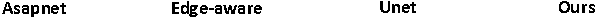
\includegraphics[width=.82\linewidth]{Chapters/detail-retouching-figs/One-shot-labels.pdf}

  \includegraphics[width=\linewidth]{Chapters/detail-retouching-figs/Qualitative_zoomed_BF.pdf}
    \caption{Qualitative comparison with baseline approaches on bilateral filtering. Bilateral filter is a nonlinear filter designed for smoothing the surfaces while preserving the edges. Results show that our proposed technique captures the bilateral-filtering effect more effectively, reducing the roughness of the surfaces while maintaining important details.} 

   \label{fig:QualitativeComp_BF}%
\end{figure*}

    
 %   These results are included in Table 1 for the filter types indicated in rows. The training strategy for the state-of-the-art methods is summarised in Section \ref{sec:Comparisons}. Before-after pairs along with additional results can be found in the supplementary material. Image courtesy of Arnaud Rougetet (landscape) and virtualhorizonstudio (alarm clock). (CC-BY and PixelSquid).

\begin{figure*}%[th]%[tph]{
  \centering
      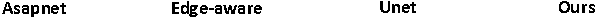
\includegraphics[width=.82\linewidth]{Chapters/detail-retouching-figs/One-shot-labels.pdf}
  \includegraphics[width=\linewidth]{Chapters/detail-retouching-figs/Qualitative_zoomed_LLF_a2_s02.pdf}
    \caption{Qualitative comparison with baseline approaches on Local Laplacian filter (LLF) ($\alpha=2, \sigma=0.2$). LLF is another edge-aware nonlinear filter designed for multiple tasks, namely edge-preserving smoothing, detail enhancement, tone mapping, and inverse tone mapping. In these examples, the parameters are chosen to have an edge-preserving smoothing effect, similar to bilateral filtering. Results show that ours offer smoother textures.} 

   \label{fig:QualitativeComp_LLF_a2}%
\end{figure*}

%These results are included in Table 1 for the filter types indicated in rows. The training strategy for the state-of-the-art methods is summarised in Section \ref{sec:Comparisons}. Before-after pairs along with additional results can be found in the supplementary material. Image courtesy of Arnaud Rougetet (landscape) and virtualhorizonstudio (alarm clock). (CC-BY and PixelSquid).

\begin{figure*}%[th]%[tph]{
  \centering
    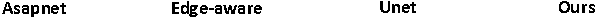
\includegraphics[width=.82\linewidth]{Chapters/detail-retouching-figs/One-shot-labels.pdf}
  \includegraphics[width=\linewidth]{Chapters/detail-retouching-figs/Qualitative_zoomed_LLF_a05_s01.pdf}
    \caption{Qualitative comparison with baseline approaches on Local Laplacian filter (LLF) ($\alpha=0.5, \sigma=0.1$). Here, the parameters are chosen accordingly to enhance the details. Our results highlight edges, such as the transition between the cloud and the sky, the numbers in the clock or the texture on the bed sheet.} 

   \label{fig:QualitativeComp_LLF_a05}%
\end{figure*}

\newpage
\subsection{Limitations and Future Work}
\begin{figure}[th] % "[t!]" placement specifier just for this example
	\centering
	\includegraphics[width=0.8\columnwidth]{Chapters/detail-retouching-figs/Limitations.pdf}
    \caption{\label{fig:limitations} The proposed technique cannot accurately handle extreme non-repeating local effects such as tattoos (top), and when example and input images are of very different semantics (bottom). Image courtesy of bgaj23 (coin). (PixelSquid).}

\end{figure}
A primary limitation of this work is its dependence on local patches at different scales, disregarding their spatial location. Hence, the method is most useful when details are retouched based on local and repeated characteristics of an image. Non-repeating spatially-dependent strong effects, e.g., tattoos or portrait stylisations with spatially varying lighting~\cite{Shih14Style}, cannot be handled by the current technique (see Figure \ref{fig:limitations}).


Since the method relies on a single example image pair, transferring filters applied to arbitrary images~\cite{Yan14Automatic} is out of the scope of this work. Example and input images are required to have similar semantics for predictable transfer. Extending the technique to more than one pair of example images will require us to have consistently retouched details on all those example images. Finally, the example before and after images are required to be perfectly aligned. This requirement can be alleviated by incorporating an ICP~\cite{Besl92AMethod}-like approach into the optimisation in Section~\ref{sec:Methodology}. 

Although the main focus in this paper is learning artist-driven subjective retouching edits, the proposed technique is general. It can be extended to transfer arbitrary image transformations, significantly where details are modified. Thus, I plan to investigate the technique further as a general transfer method for image-to-image translation. The patch-adaptive nature of the mappings makes them amenable to analysis.



\section{Summary}
\TODO{Change this paragpraph, motivate why we need detail retouching, how we achieve this, emphasising novelty with enthusiasm...}
I presented a neural field based technique for example-based automatic retouching of images. By formulating the transfer problem in the patch space, I show that blending multiple transformation matrices with patch-adaptive weights can be utilised to learn an accurate and generalisable map. This allows us to use images of different scenes, people, views, and environmental conditions as the example pair and input. I illustrated the technique's utility on various retouching examples. I believe that our image map representation can be helpful in many other image processing problems.

% \begin{figure*}%[th]
%   \centering
%   \includegraphics[height=0.8\textheight, width=\linewidth,keepaspectratio]{Images/AdditionalResults_op2.pdf}
%   \caption{
%            Retouches reproduced by our algorithm based on single before-after pairs. }
%            \label{fig:AdditionalRes}%
% \end{figure*}

% \section{Appendices}

\chapter{Text-guided Transient Attribute Transfer}\label{zero-shot}

In the previous chapter, I discussed appearance manipulation at the image level through the proposal of a low-level editing framework. The retouching framework is designed to enhance photographs by editing intricate details while refining high-level features, such as lighting or content. Conversely, this chapter focuses on a high-level manipulation task known as transient attribute transfer. In this task, we observe varying changes to the scene, including relighting, content addition or removal, and more. These edits are still learned implicitly without decomposing images into the 3D scene components.

The appearance of a scene can change dramatically over the course of a day or across seasons. While main elements, such as buildings, lakes, or forests generally remain the same, we often notice illumination changes that alter the appearance of the scene’s contents. Additionally, we might observe content being added or removed between seasons or throughout the day. For example, a scene may be covered with snow in a transient attribute change from "summer" to "winter". These changes are difficult to estimate implicitly due to the entanglement of content, illumination, and reflectance. In this chapter, I explore a conditional generative model for transferring transient attributes based on a target attribute. Specifically, I use variants of pre-trained latent diffusion models conditioned with text prompts indicating the target attribute.

I first fine-tune a stable diffusion model using the v1.5 checkpoint weights \cite{rombach2022high} and ControlNet \cite{zhang2023adding} on the Transient Attribute Dataset \cite{laffont2014transient} of 8,571 images. However, I observe that these highly complex models can easily overfit to a small dataset even in a fine-tuning setting. This challenge leads me to explore a zero-shot setup that does not require an additional dataset and use these pre-trained foundation models as a prior to guide the desired transfer instead. I evaluate the mentioned techniques qualitatively on the test images from the Transient Attribute Dataset \cite{laffont2014transient} . The zero-shot approach effectively transfers the attributes while preserving high-level content.

\section{Introduction}\label{sec:zero-shot-intro}


Attributes are high-level descriptions of visual concepts. In contrast to categories, which broadly classify objects or scenes based on high-level features, attributes often remain continuous or variable, changing across instances of the same category. For instance, in the "outdoor scene" category, attributes can be associated with seasonal transitions (e.g., winter to spring), weather changes (e.g., rainy, sunny), or times of day (e.g., daylight, sunset, night). In this work, I focus on such transient attributes that dynamically shape the visual appearance of an outdoor scene.


\begin{figure}[ht]
  \includegraphics[width=\textwidth]{Chapters/zero-shot-tat-figs/tat-teaser.pdf}
  \caption{Transition of the illumination throughout the day or the weather changes across seasons alter the scene appearance significantly in terms of colour, tone, texture, and style. However, main content, such as the structure, permanent objects, etc. remains unchanged. Transient attribute transfer aims to capture alterations related to such temporal effects. Images from the Transient Attribute Dataset \cite{laffont2014transient}.}
  \label{fig:zero-shot-teaser}
\end{figure}

Transient attributes influence our perception of a scene by altering appearance-related properties, such as colour, texture, and overall atmosphere, i.e., style and tone. From the slow transition of sunrise to daylight, the accumulation of snow on the ground, to the clearing sky after an overcast day, these attributes define the dynamic and captivating nature of the visual world. Recent works in the fields of computer vision and graphics have engaged with the transfer of such attributes, either under the umbrella term of high-level image editing or as standalone tasks. Capturing such temporal changes plays a crucial role in a range of applications, such as photography, filmmaking, gaming, and virtual and augmented reality, for producing photorealistic simulations. However, the accurate transfer of transient attributes is highly challenging due to the requirement for a deep understanding of the scene components as well as the need to maintain essential content.

This chapter aims to address these challenges by exploring recent advancements in generative models, more specifically diffusion-based approaches. The observation that fine-tuning these foundation models with a small dataset can lead to overfitting motivates me to leverage the pre-trained models to guide the transfer process in a way that improves generalisability. Therefore, I focus on a zero-shot approach that eliminates the need for extensive additional datasets, instead utilising the robust priors embedded in foundation models. I evaluate this approach through qualitative comparisons with fine-tuned models and demonstrate its ability to effectively capture transfers, such as seasonal changes and varying lighting and weather conditions, while preserving the scene's core features.

%By advancing the understanding and manipulation of transient scene attributes, this research contributes to the broader goal of enhancing the realism and flexibility of visual content generation, paving the way for more immersive and contextually adaptive visual experiences.

In summary, this chapter contributes to the broader goal of manipulating appearance in a data-efficient manner by:

%Multiple Transformation Blending
\begin{itemize}

   \item Exploiting a pre-trained diffusion model in a zero-shot setting, requiring only an input image and a single-word text prompt describing the target attribute.
    
   \item Capturing the ever-changing transitions in an outdoor scene without any explicit decomposition of scene components.

\end{itemize}


\section{Related work}\label{zero-shot-RW}
This work falls into the broader category of text-guided image-to-image translation. Here, I will review the related works on text-guided image generation and manipulation.

\subsection{Text-to-image synthesis}

Recent years have seen significant advancements in text-to-image synthesis, from the initial Generative Adversarial Network (\gls{GAN})-based approaches \cite{li2020manigan,xu2018attngan,zhang2017stackgan,zhang2018stackgan++} to the latest diffusion \cite{gu2022vector,ho2020denoising,nichol2021improved,ramesh2022hierarchical,rombach2022high,saharia2022photorealistic,song2020denoising,zhang2023adding} and transformer models \cite{ding2022cogview2,esser2021taming,ramesh2021zero,yu2022scaling}. Notably, DALL·E 2 \cite{ramesh2022hierarchical} and Imagen \cite{ho2022imagen} condition the diffusion models with text prompts. Pre-trained CLIP models \cite{radford2021learning} are also explored for guidance in image generation with text descriptions \cite{crowson2022vqgan,ramesh2022hierarchical}. More recently, Stable Diffusion \cite{rombach2022high}, trained on a large number of image-text pairs \cite{schuhmann2021laion}, was released to the public and has since become a key tool in the field for both image generation and manipulation. Later, ControlNet \cite{zhang2023adding} includes spatial conditioning controls, such as edges, depth, segmentation, and human pose, to Stable Diffusion for image generation with enhanced control. Our work utilises the latest advancements in conditional image generation and explores their pre-trained capacity to transfer transient attributes.


\subsection{Text-guided image manipulation}
Pre-trained generator models and CLIP \cite{radford2021learning} have been deployed for text-guided image manipulation, with extended applications including video editing and style transfer \cite{bar2022text2live,gal2022stylegan,kwon2022clipstyler,liu2021fusedream,patashnik2021styleclip}. For instance, StyleCLIP \cite{patashnik2021styleclip}, based on a \gls{GAN}-based generative model StyleGAN \cite{karras2020analyzing}, modifies input latent vectors with a CLIP-based loss, while VQGAN-CLIP \cite{crowson2022vqgan} guides VQ-GAN \cite{esser2021taming} using CLIP for high-quality image generation and editing. Furthermore, diffusion models have been extensively studied for text-driven image manipulation \cite{avrahami2022blended,gal2022image,kawar2023imagic,kim2022diffusionclip,liu2023more,meng2021sdedit,nichol2021glide,ruiz2023dreambooth}. Imagic \cite{kawar2023imagic} obtains text embeddings that align with the input image and the target text prompt and finetunes a pre-trained diffusion model to capture the desired edits. InstructPix2Pix \cite{brooks2023instructpix2pix} finetunes Stable Diffusion \cite{rombach2022high} with human instructions generated with the help of GPT-3 \cite{brown2020language}.

Similar to our work, DiffEdit \cite{couairon2022diffedit}, MasaCtrl \cite{cao2023masactrl}, and ZeCon \cite{yang2023zero} perform tuning-free text-guided image manipulation without requiring additional extensive datasets. DiffEdit \cite{couairon2022diffedit} utilises DDIM inversion \cite{dhariwal2021diffusion,song2020denoising} along with automatically generated masks to capture local image edits. MasaCtrl \cite{cao2023masactrl} introduces a mutual self-attention method guided by a mask that is extracted from cross-attention maps in diffusion models. ZeCon \cite{yang2023zero} introduces a zero-shot contrastive loss that works in a patch-based feature space for image style transfer. DiffEdit \cite{couairon2022diffedit} and MasaCtrl \cite{cao2023masactrl} aim for local edits with mask guidance, potentially missing global transfers that are more dominant in the transitions between transient attributes. ZeCon \cite{yang2023zero} edits high-level content without concerns about photorealism, consequently not preserving the main structures. In contrast, I explore a tuning-free method that can 1) maintain photorealism and the essential content, and 2) capture global transfers, such as illumination changes, without any mask guidance.




\section{Methodology}
I first finetune two pre-trained models,  a stable diffusion model with the v1.5 checkpoint weights \cite{rombach2022high} and ControlNet \cite{zhang2023adding} on the Transient Attribute Dataset \cite{laffont2014transient}. 

\subsection{Transient attribute dataset} 

The dataset consists of 8,571 images captured from 101 webcams, all annotated with 40 attribute labels. In order to capture static viewpoints over long periods, \citeauthor{laffont2014transient} \cite{laffont2014transient} chose a group of outdoor webcams from the following existing sources: the Archive of Many Outdoor Scenes \cite{jacobs2007consistent} and the Webcam Clip Art Dataset \cite{lalonde2009webcam}. The dataset includes images of scenes with large variations, ranging from mountainous views to urban areas, with resolutions varying between $640 \times 360$ and $4,000 \times 3,000$. Images captured from the same webcam are also manually aligned to a reference frame using a warping method.

\paragraph{Attribute labels.} Attributes are selected through crowdsourcing from an initial list of 92 scene attributes. In a crowdsourced experiment on Amazon Mechanical Turk, \citeauthor{laffont2014transient} \cite{laffont2014transient} observe that some properties rarely occur or do not vary across scenes, while weather-, lighting-, or emotion-related properties can change dramatically across the images of the same scene. This leads to a reduced number of attributes (40) in five categories: lighting, weather, seasons, subjective impressions, and additional attributes.

The attributes are as follows: \textit{dirty, daylight, night, sunrise sunset, dawn dusk, sunny, clouds, fog, storm,snow
, warm, cold, busy, beautiful, flowers, spring, summer, autumn, winter, glowing, colourful, dull, rugged, midday, dark
, bright, dry, moist, windy, rain, ice, cluttered, soothing, stressful, exciting, sentimental, mysterious, boring, gloomy, lush}.

Each image is later annotated with the corresponding attributes by workers on Amazon Mechanical Turk. As attributes lie on a continuous spectrum, the workers are asked to respond with "totally / a little / not at all" to the question "how much does each image exhibit this attribute?" These responses are later assigned label values of 1 / 0.5 / 0, and aggregated scores ranging from 0 (attribute not present) to 1 (attribute present) are estimated using a two-stage estimator. More details about the workers' performance and the estimation approach can be found in Section 3.2 of the main paper \cite{laffont2014transient}.

\subsection{Transient attribute transfer}

\paragraph{Finetuning.} Following the same convention for the attributes list, I select the annotations with scores > 0.8 to generate the associated text prompts for the images. In cases where images have multiple annotations with high scores, I merge them with a comma separator. For example, if an image has high scores for both the "sunny" and "daylight" annotations, then the text prompt is "daylight, sunny". I finetune the models with 8,571 images conditioned on the text prompts (attribute labels). For the finetuning of the models, I reform the dataset following the instructions provided in the models' official GitHub repository. I only finetune the U-Net parameters, freezing the parameters of all other components (encoders and decoders).

\begin{figure}[ht]
  \includegraphics[width=\textwidth]{Chapters/zero-shot-tat-figs/TAT-overview.pdf}
  \caption{The fine-tuning of both Stable Diffusion v1.5 and ControlNet includes an input image (source) along with a text prompt extracted from the annotations with the objective of learning the target attribute. Note that the figure only consists of a representative of the diffusion models. The network architecture of ControlNet remains the same as described in the main paper \cite{zhang2023adding}.}
  \label{fig:finetuning-overview}
\end{figure}


%\TODO{GPU info and how long you trained}

%\TODO{explain DDIM and DDPM in background}

\paragraph{DDIM inversion.} To guide the input image with a latent diffusion model, I utilise \gls{DDIM} inversion \cite{dhariwal2021diffusion,song2020denoising} , which inverts the DDIM sampling process by adding noise to the input image. Here, the idea is to start the sampling process from the noisy input image instead of pure random noise. Figure \ref{fig:ddim-inversion} shows that the input image gradually turns into random noise as the number of time steps increases. Instead of using the random noise generated at the last step, if I start from, let’s say, somewhere in the middle, I can preserve the main structures of the input image, for example, third subfigure in Figure  \ref{fig:ddim-inversion}). Later, while sampling an output image with this intermediate latent, the priors embedded in the pre-trained model can steer the noisy input image towards a target image with the text guidance.

\begin{figure}[ht]
  \includegraphics[width=\textwidth]{Chapters/zero-shot-tat-figs/DDIM_forward.png}
  \caption{In the forward process of a diffusion model, an input image gradually turns into a random noise by adding small amounts of Gaussian noise at each time step. Here, the total number of time steps is 100. In DDIM inversion, the sampling process replaces the random noise with an intermediate time step, such as $t_s = 49$, for its starting point.}
  \label{fig:ddim-inversion}
\end{figure}

Note that I use a latent diffusion model; hence, the noising process indeed occurs in the latent space. Here, I decode the noised latents with the VAE decoder of the model for visualisation. 

\paragraph{DDIM sampling.}
At a given time step $t$, the noisy image $\bm{x}_t$ is the original image ($\bm{x}_0$) mixed with some noise ($\epsilon$), mathematically defined as follows (from the DDIM paper \cite{song2020denoising}):

\begin{equation}
\bm{x}_t = \sqrt{\alpha_t}\bm{x}_0 + \sqrt{1 - \alpha_t}\epsilon
\end{equation}
where $\epsilon$ is some gaussian noise with unit variance, $\alpha_t$ is the noise scheduler. 

Sampling starts with pure noise at time step $T$ and gradually approaches $t = 0$. The next $\bm{x}_{t-1}$ in the sampling trajectory is calculated by predicting the noise $\epsilon_{\theta}(\bm{x}_t)$ with the learned model, which is used to predict $\bm{x}_0$. The noise prediction is incorporated into the "step" towards $\bm{x}_t$. Additional noise can also by added with a scale $\sigma_t$:

\begin{equation}
\bm{x}_{t -1} = \sqrt{\alpha_{t - 1}}\biggl(\frac{\bm{x}_t - \sqrt{1 - \alpha_t}\epsilon_{\theta}^{(t)}(\bm{x}_t)}{\sqrt{\alpha_t}}\biggl) + \sqrt{1 - \alpha_{t - 1} - \sigma_t^2} \, . \, \epsilon_{\theta}^{(t)}(\bm{x}_t) + \sigma_t \, \epsilon_t
\label{eq:ddim-sample}
\end{equation}
Here, the first term inside the parenthesis is the "predicted $\bm{x}_0$" multiplied with the noise scheduler, and the second term is the "direction pointing to $\bm{x}_t$". In my experiments, I do not add any additional noise term ($\sigma_t = 0$) to keep the sampling process fully deterministic. That is, samples follow a fixed procedure from $\bm{x}_T$ to $\bm{x}_0$.

Another important term to mention before discussing the experimental results is the guidance scale. A pre-trained U-Net model predicts the noise $\epsilon_t$ at each time step. In the text-conditional case, the noise prediction includes one term for the unconditional prediction and one for the text-conditioned prediction. The output noise prediction becomes the weighted average of these two, with a guidance scale $\sigma_s$:

$$\epsilon_{pred} = \epsilon_{uncond} + \sigma_s * (\epsilon_{text} - \epsilon_{uncond} )$$.

Here, I work with the classifier-free guidance.

%here: \href{https://github.com/lllyasviel/ControlNet}{ControlNet}, \href{https://github.com/timothybrooks/instruct-pix2pix}{Stable Diffusion v1.5}. 


\section{Experiments}\label{zero-shot-exp}

\subsection{Finetuning}
During finetuning, ControlNet learns a highly accurate mapping between the input and target images according to text guidance. Figure  \ref{fig:controlnet-train} shows that even the details, such as tree branches, small buildings, or windows, remain as they should. The effect of text guidance is also clearly visible in the model outputs, such as "daylight" enlightening the scene (first two columns) or "night" darkening the street (right-most column).
 
\begin{figure}[ht]
  \includegraphics[width=\textwidth]{Chapters/zero-shot-tat-figs/Controlnet2.png}
  \caption{ControlNet samples from the training examples guided with the associated text prompts. Rows demonstrate input images, target images and the model outputs, in order. The subtitles indicate the attributes guiding the model.}
  \label{fig:controlnet-train}
\end{figure}

Although ControlNet performs extremely well on the training examples, its complex architecture, with a significantly high number of parameters, causes overfitting to the dataset of approximately 8000 images, leading to a performance decrease on the test dataset with losses in details and structures (Figure \ref{fig:zero-shot-comparison} - third right-most column). For instance, the car and the hut in the second row from the bottom appear to have been replaced with an unfinished construction. Another example would be the "night" prompt, where additional buildings are placed in what was supposed to be the parking area.

In terms of overfitting, the finetuned Stable Diffusion (second right-most column in Figure \ref{fig:zero-shot-comparison}) can preserve the wooden house in the "winter" prompt and maintain the car structure in "daylight." It can also perform content creation with respect to text guidance, comparable to ControlNet. However, both models can overdo the content creation with some newly added structures, such as clouds, covering large areas in the input image.

\subsection{Zero-shot latent diffusion}
In the zero-shot case, the similarity of the model output to the input image is controlled by the start step  $t_s$, which counts from the end step  $T$. That is, the input of the sampling process is the intermediate latent that was denoised for $t_s$ steps, starting with pure noise. I keep the total number of steps as 150 in all experiments. I also experimented with larger and smaller time steps; however, I observed that as long as the ratio of the start step to the total number of steps is the same, the results remain similar. Therefore, I only experimented with the start step to maintain the core features.


The guidance scale is another crucial parameter for the success of the zero-shot setting, as it transforms the input image according to the desired attribute. I tried four different values (10, 20, 30, 40) and observed that there is no one-size-fits-all value for all images. This also applies to the start step and poses a trade-off between the preservation of the essential content and the strength of the desired transfers. I chose the zero-shot results in Figure \ref{fig:zero-shot-comparison}  (right-most column) based on the subjective judgement of this trade-off.

\subsection{Grid search}

\begin{figure}[ht]
  \includegraphics[width=\textwidth]{Chapters/zero-shot-tat-figs/grid-search.png}
  \caption{Grid search on DDIM inversion for the start step and the guidance scale. Here, the text prompt is "sunrise sunset".}
  \label{fig:zero-shot-grid-search}
\end{figure}

I ran an additional grid search on both parameters to find a balance between the text guidance and similarity to the input image. I experimented with $20, 50, 80, 100, 120$ for the start step out of the total number of 150 steps, and $10, 20, 30, 40$ for the guidance scale. Figure \ref{fig:zero-shot-grid-search} shows the grid search results for a test image, where we observe that increasing the guidance scale changes the appearance more strongly, whereas increasing the start step reduces the generation ability of the model.



\subsection{Qualitative comparison}
\paragraph{Baselines.} I also compare the finetuning and the zero-shot results with \citeauthor{laffont2014transient} \cite{laffont2014transient} and InstructPix2Pix \cite{brooks2023instructpix2pix} qualitatively. \citeauthor{laffont2014transient} \cite{laffont2014transient} learns the transforms from a pair of \textit{ Match - Target} images, as shown in the second and third columns. It has the disadvantage of requiring two additional images. On the other hand, InstructPix2Pix \cite{brooks2023instructpix2pix} is a diffusion-based model designed to edit images according to instructions. It is finetuned with a large dataset of image-target pairs along with their associated instructions. To adapt their model to our task, I convert the attributes to instructions by adding "make it" to the front of the adjective version of the attribute. For instance, if the prompt is initially "summer," then the InstructPix2Pix input becomes "make it sunny." Without this adjustment, I observed little to no changes in the input images.


 
 \begin{figure}[ht]
  \includegraphics[width=\textwidth]{Chapters/zero-shot-tat-figs/zeros-shot-qual-comp-updated.pdf}
  \caption{Qualitative comparison with the baseline methods on the test images of the Transient Attribute Dataset \cite{laffont2014transient}. Additional results can be found in Appendix \ref{TAT:add_res}.}
  \label{fig:zero-shot-comparison}
\end{figure}

Figure \ref{fig:zero-shot-comparison} shows that Zero-shot (right-most column) overall attains compelling results, comparable with InstructPix2Pix (fifth column). It maintains the core structures while transferring the target attributes to the input image. \citeauthor{laffont2014transient} \cite{laffont2014transient} can also accurately capture the transfer, but their edits remain limited to the \textit{Match - Target} pair, being unable to add some additional content, such as snow or raindrops. Both ControlNet (third column from the right) and Stable Diffusion (second from the right) are better capable of generating new content (clouds, snow, daylight, etc.). However, these models are less reliable in terms of content preservation. 



\section{Limitations and future work}
The grid search of the parameters in DDIM inversion is indeed sub-optimal, requiring manual labour for each image. Automatically optimising the parameter values based on a quantitative metric would be the future work of this project. Additionally, transient attributes usually rely on a continuous spectrum with less distinction between attributes as opposed to categories. In the future, I would like to explore the controllability of the transitions between the attributes, such as a slider interpolating appearances between two attributes, as done in the HyperBRDF work (BRDF editing, Section \ref{sec:brdf-editing}).

\section{Summary}

Transient attributes are the essence of the scene atmosphere, shaping its appearance dramatically in a natural way. Such changes to the appearance include highly complex patterns due to the coupled scene components, i.e., unknown illumination, reflectance, and geometry. In this chapter, I present highly accurate as well as creative transient attribute transfers captured by variants of pre-trained latent diffusion models. The observation that fine-tuning is costly and can overfit to a small dataset motivates me to utilise the pre-trained model as a prior in a zero-shot setting. The DDIM inversion offers a balance between the creation of new content and the preservation of the core features with a tweak of only two parameters (start step and guidance scale). This approach has the potential to advance scene appearance manipulations by eliminating the requirement of additional extensive datasets. 

%\TODO{explain fine-tuning GPU usage somewhere please}
% \begin{figure*}%[th]
%   \centering
%   \includegraphics[height=0.8\textheight, width=\linewidth,keepaspectratio]{Images/AdditionalResults_op2.pdf}
%   \caption{
%            Retouches reproduced by our algorithm based on single before-after pairs. }
%            \label{fig:AdditionalRes}%
% \end{figure*}

% \section{Appendices}

\chapter{HyperBRDF: Neural Generalizable Material Representation}
\label{ch:HyperBRDF}

Appearance is the byproduct of illumination and reflectance, in which the two interact with each other, covering the shape of the objects. Photographs can only capture the appearance with scene components coupled together. Previous chapters discuss appearance manipulations at the image level without any explicit effort for the decomposition of human-distinguishable scene properties. Image-based editing techniques are instrumental in many real-world applications; however, they suffer from the lack of explicit control over scene properties, such as light sources, material types or object geometries. This chapter goes beyond the image-level editing of appearance and brings a physics and graphics aspect to appearance representations. More specifically, I propose a neural representation of reflectance, which can be incorporated into renderers for photorealistic simulation of the scene appearance.

Bidirectional reflectance distribution functions (\gls{BRDF}) define the reflectance as a function of illumination and viewing directions. This chapter presents HyperBRDF, a technique to estimate measured \gls{BRDF}s from a sparse set of samples. HyperBRDF offers accurate \gls{BRDF} reconstructions that are generalisable to new materials. This opens the door to \gls{BRDF} reconstructions from a variety of data sources. The success of the approach relies on the ability of hypernetworks to generate a robust representation of \gls{BRDF}s and a set encoder that allows us to feed inputs of different sizes to the architecture. The set encoder and the hypernetwork also enable the compression of densely sampled \gls{BRDF}s. I evaluate the technique both qualitatively and quantitatively on the well-known MERL dataset of 100 isotropic materials. HyperBRDF accurately 1) estimates the \gls{BRDF}s of unseen materials even for an extremely sparse sampling, 2) compresses the measured \gls{BRDF}s into very small embeddings, e.g., 7D. 


\TODO{Intro paragpragh needed to connect this chapter with main theme of the thesis. Start with motivation, leave it to end while writing the main Intro}
\TODO{give credit to Alejandro  for MainFig, GGX fittings and Casual Capture, also Chenliang for t-SNE figure}


\section{Introduction}
\label{sec:intro}


In computer graphics and vision, achieving realistic renderings for intricate surface materials hinges on accurately describing the interaction of light with the surfaces. This is conventionally conveyed through the modeling and reconstruction of a 4D Bidirectional Reflectance Distribution Function (BRDF), which quantifies the relationship between the incident and outgoing light intensities for a specific material. In this chapter, I propose a novel generalizable BRDF representation model that can estimate the BRDFs of new materials from highly sparse and unstructured point-based samples \footnote{Point-based samples refer to the BRDF values acquired at specific points on a surface with known viewing and lighting directions.} and compress the densely sampled values into very small latent embeddings.


While there has been prior work that attempts to tackle similar tasks by estimating the free parameters of analytic BRDF functions or the principal components of BRDF functions from images or reflectance measurements, the oversimplified models of the complex BRDF function lead to inaccuracies when predicting real materials, thereby diminishing the realism in renderings~\cite{ngan2005}. Moreover, the process of fitting through nonlinear optimization is inherently unstable, computationally expensive, and prone to local minima, hindering the accurate reconstruction of material appearance~\cite{dupuy2015, guarnera2016}. Measured BRDFs of real-world materials can also be fraught with errors due to equipment limitations, adding to the complexity of the fitting process~\cite{nielsen2015optimal}. 

\begin{figure}
  \centering
   \includegraphics[width=\linewidth]{Chapters/hyperbrdf-figs/teaser_cropped.png}
   \caption{A room scene rendered with materials reconstructed by HyperBRDF, including sparse reconstruction (table top and legs, door, door and picture frames, hinge), compression (two teapots on the left, door handle) and BRDF interpolation (right-most teapot). Scene courtesy of Benedikt Bitterli.}
   \label{fig:teaser}
\end{figure}

Recent advances in deep learning have enabled the accurate representation of complex continuous signals (\textit{e.g.} images, surfaces, volumes, materials, \textit{etc.}) using a Neural Field~\cite{sitzmann2020siren, ffn, cnf2023}, \textit{i.e.} a neural network mapping coordinate inputs to sampled values, without compromising model compactness. Consequently, neural fields have gained substantial popularity for representing continuous BRDFs in recent works~\cite{sztrajman2021neural, cnf2023}. However, reconstructing a neural field representation for BRDFs typically requires training the network with a regression loss function to overfit to a single material, which demands dense sampling and extensive computational resources, while being unable to generalize to new materials.

More recently, Generalizable Neural Fields~\cite{rebain2022attention} (GNFs) have emerged as a promising solution to the aforementioned challenges. Rather than overfitting to individual signals, GNFs are designed to learn a generalized mapping, either deterministic or probabilistic, between sampled signals and their full neural field representations in a fashion similar to supervised learning.
The key strategy of GNFs involves conditioning the neural fields with a latent embedding of the signal samples. Popular conditioning mechanisms include concatenated latent vectors~\cite{park2019deepsdf}, hypernetworks~\cite{ha2017hypernetworks}, and attention-based set latent representations~\cite{jiang2021cotr}. Once the conditional neural field is properly learned, reconstruction of the full signal can be achieved at inference time, and even with highly sparse and unstructured samples.


Inspired by GNFs, I propose a novel framework, HyperBRDF, for generalizable neural BRDF representation for both the estimation of unseen materials from sparse and unstructured samples and the compression of measured BRDFs into low-dimensional latent space. In this framework, I employ a multi-layer perceptron (MLP) model as the neural field backbone for BRDF representation, a hyper-network for conditioning, and a set encoder that allows for mapping an arbitrary number of reflectance measurements from arbitrary directions to a compact latent embedding for conditional BRDF generation. 
The built-in nonlinear interpolation capability of the hyper-network also offers robust and adaptable material editing and blending across various sample sizes.


Unlike previous work, the BRDF reconstruction of HyperBRDF is highly efficient without the need for extensive training to overfit individual materials, while also maintaining state-of-the-art performance in reconstruction accuracy for sample size below 4000; see Figure~\ref{fig:imp_comp_upt}.


In summary, HyperBRDF offers a novel solution for the challenging task of generalizable BRDF modelling with the following key contributions:
\begin{itemize}
    \item{\textbf{Generalizability and Adaptability:} HyperBRDF ensures robustness and adaptability across varying sample sizes and appearances, making it highly effective for estimating the BRDFs of unseen materials from highly sparse and unstructured sampling. Its adaptability also extends to highly compact representation of BRDFs, overall outperforming the prior state-of-the-art compression method; see Table \ref{table: oursvsnps}.}
    

    \item{\textbf{Realism and Accuracy:}
    My extensive evaluation demonstrates the superior performance of HyperBRDF in reconstructing the BRDFs of 20 test materials from a limited number of samples, ranging from 40 to 4000, outperforming prior methods in terms of appearance modeling and color preservation (by at least 2dB in peak-signal-to-noise ratio and 1 in Delta E).
    }
\end{itemize}

\section{Motivation and impact}
\label{sec:hyperbrdf-mot}

The representation of measured BRDFs is crucial in computer graphics, especially in physically-based rendering (PBR) for applications such as filmmaking, gaming, virtual and augmented reality, and product design, aiming for immersive realism. PBR provides a more precise portrayal of light-material interactions. However, real-world BRDF models are reconstructed by taking samples with a device, such as a camera or gonioreflectometer and often demand numerous samples, making acquisition, storage, and manipulation costly and challenging. For instance, the MERL dataset \cite{Matusik2003jul}, the main dataset I utilised for experiments, captures 330 high dynamic range images with a CCD camera for each material in roughly four hours. The RGL dataset \cite{dupuy2018adaptive}, the secondary dataset included in training, captures samples with a gonioreflectometer that leads to captures times of approximately 2.5 hours for isotropic materials. Therefore, HyperBRDF offers multiple impactful contributions: 
\begin{itemize}
 \item can integrate with professional setups where capturing only one material can take hours. HyperBRDF’s superior sparse reconstruction ability can help significantly reduce the manual and heavy workload of material acquisition. I also discuss the related work aligned with this research line in Section \ref{hyperbrdf-RW}.
 \item Providing BRDF compression with high accuracy and efficiency, encoding over a million samples into a 7D latent vector, saving storage space and increasing transfer speed. 
 \item Allowing easy material editing through its latent space representation.
 \end{itemize}

\section{Related Work}
\label{sec:relatedwork}


\subsection{Analytic BRDF Models}
Analytic models are the most common representation for BRDFs. Classic BRDF models include Phong~\cite{blinn77}, Cook-Torrance~\cite{cooktorrance1982}, Ward~\cite{ward1992} and GGX~\cite{walter2007microfacet}. Following models have increased their reconstruction capabilities by combining analytic formulations with data-driven representations of some or all of their components~\cite{dupuy2015, ashikhmin2007, bagher2016}. Notably, the ABC model~\cite{low2012} has been shown to provide an accurate reconstruction of measured materials, while only requiring the fitting of a handful of tunable parameters. These models are usually fast at evaluation, easily editable, and present a low memory footprint. However, they usually rely on oversimplifications of the reflectance distribution shapes, and thus have a limited capacity for the reconstruction of complex real-world materials~\cite{ngan2005, guarnera2016}. Therefore, recent works have started exploring neural representations to overcome these limitations.



\subsection{Regression-based BRDF Estimation}
For a simpler representation of measured BRDFs, BRDF decomposition methods, such as PCA decomposition 
\cite{matusik2003data, nielsen2015optimal, serrano2018intuitive}, non-negative matrix factorization \cite{lawrence2004efficient, lawrence2006inverse}, Gaussian mixture \cite{sun2007interactive}, tensor decomposition \cite{bilgili2011general, tongbuasirilai2020compact} 
and non-parametric models~\cite{bagher2016non} have been proposed. The main limitation of PCA and factorization methods is  that they have a limited capacity to represent complex functions without overfitting to the training dataset. In contrast, our method can represent the complex BRDFs even with sparse samples while maintaining generalizability.


\paragraph{Deep learning for BRDF modeling.}

Multiple methods have been recently proposed for neural BRDF representation~\cite{rainer2019neural, hu2020deepbrdf, sztrajman2021neural, zheng2021compact, maximov2019deep, chen2021invertible, fan2021neural, cnf2023}. These methods usually offer a flexible representation, and thus are well fitted to encode the complex reflectance distributions of real-world measured materials. However, an accurate fitting of these methods usually requires lengthy optimizations and a very large number of sample measurements, typically from $8 \times 10^5$ to $1.5 \times 10^6$. \cite{maximov2019deep} learned materials with baked illumination via small fully-connected networks. NBRDF \cite{sztrajman2021neural} and CNF~\cite{cnf2023} leveraged neural fields to learn individual BRDF functions. Closer to our work, DeepBRDF~\cite{hu2020deepbrdf} and Neural Processes~\cite{zheng2021compact} introduce neural network architectures to learn a compressed latent space from a dataset of multiple materials. However, these methods only address the problem of compressing BRDF samples into a low dimensional space, hence overfitting to the dataset. Our method, on the other hand, also offers a generalizable approach for the reliable reconstruction of unseen materials from sparse and unstructured real-world reflectance measurements.


\subsection{Efficient BRDF Acquisition}
Realistic reflectance acquisition commonly requires a large amount of physical acquisition samples collected from different directions, making the process time-consuming and data intensive. To take fewer samples, hence reducing the BRDF capture time, optimization of a sample pattern with a linear statistical analysis of a database of BRDFs \cite{nielsen2015optimal} and the joint optimization of the sample pattern and a non-linear BRDF model~\cite{liu2023learning} have been proposed.

\paragraph{Spatially-varying BRDFs (SVBRDF):} For efficient SVBRDF capture, several methods based on multiplexing-based, also known as illumination-based, acquisition systems \cite{kang2018efficient, kang2019learning, ma2021free, ma2023opensvbrdf, tunwattanapong2013acquiring} have been proposed. A common approach has been to optimize the lighting patterns for efficient acquisition, followed by a BRDF fitting to an analytic model. Recent works have also leveraged deep learning architectures to learn a mapping from images to texture maps of analytic SVBRDF parameters~\cite{guo2021highlight, hui2017reflectance, deschaintre2018single, deschaintre2019flexible, martin2022materia, zhou2021adversarial,gao2019deep}. 

In contrast to those works, our focus is the reconstruction of spatially uniform BRDF that can accurately represent arbitrary complex materials. The works on spatially-varying BRDFs and efficient capture could be considered orthogonal to ours, and those methods could be potentially combined with ours. 


\subsection{Hypernetworks and GNFs}
The capacity of hypernetworks to dynamically output neural network weights, which allows models to adjust to input conditions, has drawn attention. Its promise in a variety of computer vision tasks, including dynamic network adaptation and generating neural implicit fields, has been demonstrated by recent works, such as HyperGAN \cite{ratzlaff2019hypergan} and Hyperdiffusion \cite{erkocc2023hyperdiffusion}.
The concept of a generalizable neural field has also been extensively applied to the reconstruction of neural radiance fields~\cite{wang2022attention, yang2023contranerf}, but not sufficiently studied in other domains.
These research efforts serve as our source of inspiration as we apply hypernetworks and GNFs to BRDF estimation, improving the model's adaptability to various material appearances.


\section{Methodology}

\begin{figure*}[t]
  \centering

   \includegraphics[width=\linewidth]{Chapters/hyperbrdf-figs/MainFig_13_11.pdf}
   \caption{During training, the set encoder and hypernetwork decoder are trained on a set of materials to predict the weights of hyponet (MLP) so that it can reconstruct the training set. The BRDF data is provided as a set of BRDF coordinates, $H_n,D_n$, and the corresponding reflectance values $f_r(H_n,D_n)$. To reconstruct a new material from a small set of BRDF reflectance samples, the trained set encoder and hypernetwork decoder are used to predict the weights of hyponet for the unknown material. Once those weights are known, we can query BRDF at any coordinates and for any new materials, conditioned on the embedding of their sampled BRDF values.}
   \label{fig:mainfig} \end{figure*}

Based on our observation that recent work misses a generalized and adaptable BRDF representation, we propose a novel representation for measured BRDFs that learns compact embeddings of the BRDFs with a hypernetwork model.

\subsection{Pre-processing}\label{sec:pre-proc}

Measured BRDFs usually contain high dynamic range (HDR) data, including arbitrarily high values, especially for the specular components. Hence, we pre-process the BRDF data by applying a Log Relative Mapping~\cite{nielsen2015optimal} of the form:
\begin{equation}
  \rho' = \ln{\left(\frac{\rho + \epsilon}{\rho_{ref} + \epsilon} +1\right)}
  \label{eq:preprocess}
\end{equation}
where $\rho$ refers to the BRDF values, $\epsilon = 0.002$ is a small constant value to avoid zero-division, and $\rho_{ref}$ is a reference BRDF value for relative mapping. The reference BRDF value is chosen to be the median value for each angle over the entire dataset.


We also observe that input parameterization has a strong impact on the reconstruction quality since it guides the neural network model to learn different aspects of the reflectance function. Therefore, similar to NBRDF~\cite{sztrajman2021neural}, we express the BRDFs as functions of the Cartesian vectors $H$ and $D$ in the Rusinkiewicz parameterization \cite{rusinkiewicz1998new},
\textit{i.e.}, $\rho=f_r(H, D)$, where $H, D \in S^2$ indirectly encode the information about the incident and outgoing light directions.

Importantly, in this parameterization the directions of specular reflection have a single fixed representation as $H=(0,0,1)$, which provides an easier pattern for the network to learn than the traditional $\omega_i, \omega_o$ encoding.


\subsection{Hypernetwork}
\label{sec:hypernet}

In Figure~\ref{fig:mainfig}, we show the diagram of our hypernetwork model~\cite{sitzmann2020siren} for BRDF representation, with three main components: 1) a set encoder that generates compact latent representations $Z$ of BRDFs based on an arbitrary number of directional samples, 2) a hypernetwork decoder that decodes the latent to estimate the parameters of a neural field,
and 3) a neural field controlled by the decoder that represents the BRDFs of the material, which we refer to as a hyponet, following the convention of prior work~\cite{sitzmann2020metasdf}.


\subsubsection{Set Encoder} %add number of layers

The set encoder takes as input an arbitrary set of samples, $n=1..N$, taken from a BRDF measurement. Each measurement consists of directional coordinates ${H_n, D_n}$, given in the Rusinkiewicz parameterization~\cite{rusinkiewicz1998new}, and their corresponding BRDF values $f_r(H_n,D_n)$. The set encoder is composed of four fully-connected layers with two hidden layers of feature size 128 for each. The input is the concatenation of BRDF values $(N, 3)$ and coordinates $(N, 6)$. The activation function applied after each layer is ReLU. Each sample is encoded into a 40-dimensional embedding, and the sample set is reduced to a single embedding by applying a symmetric operation (averaging).
% \FZ{Permutation invariant operations are common in point set networks. Consider referring to the literature to motivate our design over alternatives.}
The use of a set encoder, which is commonly adopted in point set networks \cite{zaheer2017deepsets}, ensures permutation invariance and provides a high degree of flexibility in terms of the input, enabling the encoding of BRDFs with an arbitrary number of data-points, irregularly sampled, and in no pre-defined order.


\subsubsection{Hypernetwork Decoder and Hyponet} %add number of layers and type
The hypernetwork decoder converts the embeddings from the set encoder into the weights of the hyponet that represents the BRDFs of a single material. The hypernetwork decoder is composed of 10 blocks of a fully-connected neural network with three layers. Each block outputs the corresponding weights and biases of hyponet. The hyponet consists of five fully-connected layers with input layer of size 6 for coordinates, three hidden layers of size 60 for each, output layer of size 3 for BRDF values. Our neural representation of materials, hyponet, follows the structure of NBRDF~\cite{sztrajman2021neural}, but replaces the exponential activation in the last layer with a ReLU activation due to BRDF properties ($\rho \ge 0$). This network provides a continuous representation of a BRDF, and has been shown to provide state-of-the-art reconstructions of measured BRDFs, with performances competitive with the fastest analytic BRDF models.


\subsection{Training}
\label{sec:traindet}


We train the hypernetwork by optimizing the following loss, which consists of a reconstruction term $\mathcal{L}_\text{rec}$ and two regularization terms $\mathcal{L}_\text{weights}$ and $\mathcal{L}_\text{latent}$ for the hyponet weights $w$ and the latent embeddings $z$ ~\cite{ha2017hypernetworks}:
\begin{equation}
    \mathcal{L} = \mathcal{L}_\text{rec} +
              \lambda_1 \underbrace{\frac{1}{W} \sum_{j=1}^W w^2_j}_{\mathcal{L}_\text{weights}} +
              \lambda_2 \underbrace{\frac{1}{Z} \sum_{k=1}^Z z^2_k}_{\mathcal{L}_\text{latent}}
    \label{eq:loss}
\end{equation}

We define the reconstruction loss as the mean squared error between the cosine weighted predicted and ground-truth BRDF values:

\begin{equation}
    \mathcal{L}_{\text{rec}} = \sum_{n=1}^{N}\sum_{m=1}^{M}\frac{\left|\left|\rho^{\text{pred}}_{n, m} \cos{\theta_{n, m}} - \rho^{\text{true}}_{n, m} \cos{\theta_{n, m}}\right|\right|_{2}}{NM}
    \label{eq:Lrec}
\end{equation}

where $\rho^{\text{pred}}_{n, m}$ and $\rho^{\text{true}}_{n, m}$ indicate the predicted and ground truth BRDF values of the $n$-th sample of the $m$-th material, both processed as described in Eqn \ref{eq:preprocess}, and $\theta$ measures the angle between the incident ray and the surface normal. The cosine term weighs BRDFs based on the assumption of uniform incoming radiance and leads to more visually accurate results \cite{ngan2005experimental}.


We train our network for 80 epochs with $1\,458\,000$ samples per material. It takes around 15 minutes with an NVIDIA A100 80GB GPU support. 


\paragraph{Inference:}
When inferring the reflectance values, our model first estimates hyponet weights from sparse samples of a test material, which takes around 0.01 seconds without GPU. Later, we feed query coordinates to the hyponet to predict the BRDF values of the material. With the conversion of the predicted BRDF into a renderable format, this process takes around 9 seconds without GPU. The continuous representation of BRDFs with the hyponet offers a nonlinear built-in interpolation and, hence, accurately reconstruct unseen materials from even a few samples.
\section{Experiments}\label{sec:exp}


\subsection{Datasets and baselines}

To show the effectiveness of the proposed method, I use MERL \cite{Matusik2003jul} and RGL (51 isotropic materials) \cite{dupuy2018adaptive} datasets, which are the most commonly used \gls{BRDF} datasets that include isotropic materials. The MERL dataset \cite{Matusik2003jul} consists of 100 real-world materials, covering a wide range of appearances. Each material includes reflectance measurements from a dense set of directions, parameterised as the spherical angles ($\theta$, $\phi$) of the $H$ and $D$ vectors from the Rusinkiewicz parameterisation \cite{rusinkiewicz1998new}. Each colour channel has a resolution of $90 \times 90 \times 180$, leading to 1,458,000 reflectance measurements. 



\subsection{Sparse BRDF reconstruction}\label{sec:brdf_rec}

To understand the reconstruction capacity of HyperBRDF, I first train the model with all available samples (1,458,000). I observe that reducing the number of samples by around half (640,000) results in a similar performance (Table \ref{table: ours_large_samples}). For comparison with baselines, I train the hypernetwork model with 80 MERL materials that are randomly selected. I leave the remaining 20 materials for testing. I also train HyperBRDF with a mixed dataset of 80 MERL materials and 51 isotropic RGL materials. I later test the trained model on the same test dataset (20 MERL materials). I apply a separate log relative mapping to RGL materials by computing the median over the isotropic RGL dataset.
 
I qualitatively compare the results against the ground truths through renderings of the materials. The renderings are obtained by a Mitsuba renderer with an environment map illumination. HyperBRDF can capture the diffuse colours of varying unseen appearances even for the materials with specular components. 


The main advantage of the hypernetwork architecture is that it is flexible in the number of samples fed to the network. That is, we can reconstruct unseen materials with fewer samples than the sample number used during training. Thanks to its built-in nonlinear interpolation that comes from the hyponet, I obtain high quality reconstruction results with fewer samples. 

Considering the hypernetwork architecture, we understand that the gap between reconstruction results with sparse samples relies on the embeddings $z$ (latent vectors). I hence analyse the embeddings for the materials reconstructed with varying number of samples. Figure \ref{fig:tsne-vis-imputation} illustrates the t-SNE clustering of the test embeddings with different number of samples. It is visible that the embeddings of the same material reconstructed with different sample sizes lie close in the t-SNE space.

\begin{figure}[t]
  \centering
  % \fbox{\rule{0pt}{2in} \rule{0.9\linewidth}{0pt}}
   \includegraphics[width=0.8\linewidth]{Chapters/hyperbrdf-figs/tsne6_2_den1-cropped-compressed.pdf}
   \caption{t-SNE clustering of the test embeddings with different sample sizes, including $N=8, 40, 160, 4\,000, 40\,000, 640\,000$.}

   \label{fig:tsne-vis-imputation}
\end{figure}


\subsubsection{Qualitative comparison}\label{sec:qual_comp}
\begin{figure*}[t]
  \centering
%\adjustbox{trim={0.\width} {.\height} {0.89\width} {.\height},clip}%
  %{\includegraphics[width=0.9\linewidth]{Chapters/hyperbrdf-figs/imp_comp_upt_3vals.pdf}}
%\adjustbox{trim={0.113\width} {.\height} {0.596\width} {.\height},clip}%
  %{\includegraphics[width=0.9\linewidth]{Chapters/hyperbrdf-figs/imp_comp_upt_3vals.pdf}}
%\adjustbox{trim={0.41\width} {.\height} {0.298\width} {.\height},clip}%
  %{\includegraphics[width=0.9\linewidth]{Chapters/hyperbrdf-figs/imp_comp_upt_3vals.pdf}}
%\adjustbox{trim={0.707\width} {.\height} {0.\width} {.\height},clip}%
 % {\includegraphics[width=0.9\linewidth]{Chapters/hyperbrdf-figs/imp_comp_upt_3vals.pdf}}

%\adjustbox{trim={0.\width} {.\height} {0.89\width} {.06\height},clip}%
  %{\includegraphics[width=0.9\linewidth]{Chapters/hyperbrdf-figs/imp_comp_upt_3vals_bad.pdf}}
%\adjustbox{trim={0.113\width} {.\height} {0.596\width} {.06\height},clip}%
  %{\includegraphics[width=0.9\linewidth]{Chapters/hyperbrdf-figs/imp_comp_upt_3vals_bad.pdf}}
%\adjustbox{trim={0.41\width} {.\height} {0.298\width} {.06\height},clip}%
  %{\includegraphics[width=0.9\linewidth]{Chapters/hyperbrdf-figs/imp_comp_upt_3vals_bad.pdf}}
%\adjustbox{trim={0.707\width} {.\height} {0.\width} {.06\height},clip}%
 % {\includegraphics[width=0.9\linewidth]{Chapters/hyperbrdf-figs/imp_comp_upt_3vals_bad.pdf}}
  
  \adjustbox{trim={0.07\width} {.\height} {0.816\width} {.\height},clip}%
  {\includegraphics[width=0.9\linewidth]{Chapters/hyperbrdf-figs/qual_comp_ggx_2.pdf}}
\adjustbox{trim={0.184\width} {.\height} {0.41\width} {.\height},clip}%
{\includegraphics[width=0.9\linewidth]{Chapters/hyperbrdf-figs/qual_comp_ggx_2.pdf}}
\adjustbox{trim={0.593\width} {.\height} {0.\width} {.\height},clip}%
  {\includegraphics[width=0.9\linewidth]{Chapters/hyperbrdf-figs/qual_comp_ggx_2.pdf}}
 %{\includegraphics[width=0.9\linewidth]{Chapters/hyperbrdf-figs/qual_comp_ggx_2.pdf}}
\\
\hspace{1.9cm}{\includegraphics[width=0.73\linewidth]{Chapters/hyperbrdf-figs/N_labels2.pdf}}
   \caption{Qualitative comparison results for reconstruction with small sample sizes. Thanks to the prior that the hypernetwork model learns for material appearance through training, it can accurately estimate theBRDFs of unseen materials and preserve the colours better than the baselines.}  

   \label{fig:imp_comp_upt}
\end{figure*}

\begin{figure*}[t]
  \centering
    {\includegraphics[width=0.35\linewidth]{Chapters/hyperbrdf-figs/legend.png}}\\
  {\includegraphics[width=0.32\linewidth, height=3.4cm]{Chapters/hyperbrdf-figs/PSNR_ggx.pdf}}
  {\includegraphics[width=0.32\linewidth, height=3.4cm]{Chapters/hyperbrdf-figs/DeltaE_ggx.pdf}}
  {\includegraphics[width=0.32\linewidth, height=3.4cm]{Chapters/hyperbrdf-figs/MAE_ggx.pdf}}
  {\includegraphics[width=0.32\linewidth, height=3.4cm]{Chapters/hyperbrdf-figs/RMSE_ggx.pdf}}
    {\includegraphics[width=0.32\linewidth, height=3.4cm]{Chapters/hyperbrdf-figs/RAE_ggx.pdf}}
    {\includegraphics[width=0.32\linewidth, height=3.4cm]{Chapters/hyperbrdf-figs/SSIM_ggx.pdf}}
   \caption{Average \gls{PSNR}, Delta E (CIE 2000), \gls{SSIM}, MAE, RMSE, and RAE results across different sample sizes. }
   \label{fig:imp_plots}
\end{figure*}



I first compare the results with the ground truth renderings for varying sample sizes. Figure \ref{fig:imp_comp_upt} shows that the hypernetwork can still reconstruct test materials even with $N = 40$ samples. However, as I reduce the sample number to 10, the reconstruction quality highly decreases. 

During inference time, hypernetwork fits the samples to a \gls{BRDF}. Even with a few samples, it can still accurately reconstruct test materials. Its success comes from the fact that it learns a prior for material appearance through training with a dataset of multiple materials. Therefore, I validate this generalisable approach by comparing the hypernetwork with an analytic model, GGX  \cite{walter2007microfacet}, NBRDF \cite{sztrajman2021neural} and PCA with Log Relative Mapping (IPCA) \cite{nielsen2015optimal}.

Sparse GGX results are obtained by fitting to the sparse number of measured \gls{BRDF} samples using a non-linear optimisation (L-BFGS-B method) with Log $\mathcal{L}_{1}$ loss (same loss used in NBRDF). For the results with all samples, I used the dj\_brdf mitsuba plug-in \cite{dupuy2015photorealistic}. NBRDF \cite{sztrajman2021neural} is designed to implicitly represent an individual \gls{BRDF}. It can reconstruct materials with very high accuracy (\gls{SSIM} $\approx$ 0.995) when the sample size is high. It first trains the network on a material and then estimates the \gls{BRDF} values of the same material. For a fair comparison, I first fit an NBRDF model to a material \gls{BRDF} with the query sample size, then estimate the function with the same sample size. 

I also compare the results with a PCA-based strategy (IPCA). To represent the \gls{BRDF} data, PCA-based methods  \cite{matusik2003data, ngan2006image} construct a matrix ${A} \in \mathbb{R}^{m \times n}$, where n = $180 \times 90 \times 90 \times 3$ = 4,374,000 is the feature number, m = 80 is sample number. The matrix is later decomposed into its principal components via Singular Value Decomposition. PCA itself struggles with the decomposition of high dynamic range data. Therefore, the Log Relative Mapping (IPCA) is proposed~\cite{nielsen2015optimal}, which is defined in the pre-processing step (Section \ref{sec:pre-proc}). This improves the reconstruction quality, offering competitive reconstructions against HyperBRDF as shown in Figure \ref{fig:imp_comp_upt}.

For all methods including HyperBRDF, samples are drawn from a uniform distribution over Rusinkiewicz coordinates. For IPCA results, I split train and test dataset in the same way as HyperBRDF, i.e., 80 MERL materials for train and 20 for test, and use all available samples for learning the principal components. To reconstruct the test materials from sparse samples, I first run a least-squared-error optimisation and predict the weights of the material for the corresponding principal components. To decide the number of components, I ran an additional ablation study, where 
I computed the average mean squared error over the test dataset for the reconstruction from sparse samples ($N = 40$). We observed that ($N_{PC} = 8$) gives the minimum error on the test dataset. Hence, I choose the number of principal components as $N_{PC} = 8$ and keep it same for sparse sampling results.

 
I keep the range for sparse sample numbers between $N = 40$ and $N = 4000$. Figure \ref{fig:imp_comp_upt} shows the rendering results for the minimum and maximum number of this range. Compared to GGX, IPCA and NBRDF, the hypernetwork can capture the appearances more precisely. Although this approach has difficulty estimating specular components (last two rows in Figure~\ref{fig:imp_comp_upt}), overall it offers reconstructions with much higher accuracy. 

I observe that the diffuse colours of some reconstructed materials by NBRDF can be completely off (natural-209, teflon) due to function fitting with sparse samples. Hypernetwork, on the other hand, can preserve diffuse colours better thanks to the prior it learns through training.


\subsubsection{Quantitative evaluation}

I compare the proposed method quantitatively with the aforementioned techniques in multiple image-based error metrics through rendering results. The metrics include \gls{PSNR}, Delta E (CIE 2000), \gls{SSIM}, \gls{MAE}, root mean square error (RMSE), and relative absolute error (RAE). I take the average over the test dataset for each metric. I plot the metric results across five different sample sizes (40, 160, 400, 2000, 4000). Since I optimise IPCA on the test dataset for the $N = 40$ case, it offers more competitive results. Nevertheless, HyperBRDF can reconstruct the \gls{BRDF}s of unseen materials more precisely. Figure \ref{fig:imp_plots} shows that across all sample sizes, the hypernetwork attains superior performance in terms of \gls{PSNR}, Delta E (CIE 2000) and \gls{SSIM}. 

Additionally, Table \ref{table: ours_diff_samples} shows that expanding the training set, even with materials captured from a different point-based setup, helps improve the performance of the hypernetwork. Also, note that compared to MERL materials, the colours of RGL materials are more saturated, which could explain a slight increase in Delta E.


 \begin{table*}[ht]
    \centering
    \caption{Hypernetwork sparse reconstruction - Average metric results across varying sample sizes ($N$) over the test set. We highlight \colorbox{blue!25}{best} and \colorbox{orange!25}{second best} results.}
    
    {\begin{tabular}{l@{\hskip 0.4in}c@{\hskip 0.2in}c@{\hskip 0.2in}c@{\hskip 0.1in}|@{\hskip 0.1in}c@{\hskip 0.2in}c@{\hskip 0.2in}c}\toprule
    

& \multicolumn{3}{c}{MERL} & \multicolumn{3}{c}{MERL + RGL}
\\\cmidrule(lr){2-4}\cmidrule(lr){5-7}
% \toprule
  $N$ & PSNR\textuparrow & Delta E\textdownarrow & SSIM\textuparrow & PSNR\textuparrow & Delta E\textdownarrow & SSIM\textuparrow \\

 \toprule

$40$ & 29.581 & 3.189 & 0.968 & 30.018 & 3.112 & 0.963\\
$160$ & 31.341 & 2.681 & 0.973 & 31.929 & 2.454 & 0.962\\
$400$ & 32.743 & 2.272 & \cellcolor{blue!25} 0.979 & 33.855 & 2.432 & 0.977\\
$2000$ & \cellcolor{blue!25} 34.527 & \cellcolor{orange!25}2.256 & \cellcolor{blue!25} 0.979 & \cellcolor{blue!25} 34.527 & \cellcolor{orange!25} 2.243 & \cellcolor{blue!25} 0.983\\
$4000$ & \cellcolor{orange!25} 33.170 &  \cellcolor{blue!25} 2.138 & \cellcolor{orange!25} 0.977 & \cellcolor{orange!25} 34.355 & \cellcolor{blue!25} 2.166 & \cellcolor{orange!25} 0.982\\

\bottomrule
    \end{tabular}\par}
    \label{table: ours_diff_samples}
\end{table*}

\paragraph{Sparse and full reconstruction results:}

\begin{table*}[ht]
    \centering
    \caption{Hypernetwork - Average metric results across varying sample sizes ($N$) over the test set (Sparse and full reconstruction of unseen materials).}

    \resizebox{0.75\linewidth}{!}{%
    {\begin{tabular}{l@{\hskip 0.2in}c@{\hskip 0.2in}c@{\hskip 0.2in}c@{\hskip 0.2in}c@{\hskip 0.2in}c@{\hskip 0.2in}c}\toprule

 Metrics/$N$ & $8$ & $40$ & $4000$ & $40\,000$ & $640\,000$ & $1\,458\,000$\\
 \toprule
PSNR\textuparrow & 23.090 & 29.822 & 33.170 & 33.019 & \cellcolor{blue!25}33.166 & \cellcolor{orange!25} 33.128 \\
Delta E\textdownarrow & 5.948 & 3.086 & 2.138 & \cellcolor{orange!25} 2.118 & \cellcolor{blue!25}2.117 & 2.181 \\
SSIM\textuparrow & 0.927 & 0.969 & 0.977 & \cellcolor{blue!25} 0.979 & \cellcolor{blue!25} 0.979 & \cellcolor{orange!25}0.978 \\
MAE\textdownarrow & 13.167 & 5.306 & 3.642 & \cellcolor{orange!25} 3.568 & \cellcolor{blue!25}3.492 & 3.574 \\
RMSE\textdownarrow & 22.293 & 9.601 & 6.791 & \cellcolor{orange!25} 6.618 & \cellcolor{blue!25}6.507 & 6.740 \\
RAE\textdownarrow & 0.339 & 0.134 & 0.093 & \cellcolor{orange!25} 0.091 & \cellcolor{blue!25}0.089 & \cellcolor{orange!25} 0.091 \\
\bottomrule
    \end{tabular}\par}}
    \label{table: ours_large_samples}
\end{table*}


\subsubsection{Comparison with casual capture setups}
Casual \gls{BRDF} estimation methods reconstruct \gls{BRDF}s from a captured material image; hence, they struggle with disentangling the material from unknown illumination, often requiring a data-driven prior. As a result, most recent papers make simplifying assumptions about the material, fitting to a Phong or an analytic model. Even though iBRDF \cite{chen2021invertible} explores fitting to real-world reflectance measurements, HyperBRDF still overwhelmingly outperforms their reconstruction quality with only 160 samples and above. When iBRDF is run with the same rendering setup on the same test dataset, we observe that even HyperBRDF's $N=160$ case overall offers more accurate results. Thus, casual capture remains highly impractical for professional applications mentioned earlier. Also, note that iBRDF trains their model with ground-truth measured \gls{BRDF} values, and hence their requirements for supervision are no less than HyperBRDF. 


%In casual \gls{BRDF} estimation, the main bottleneck lies in decoupling unknown illumination from the material, often necessitating a data-driven prior, thus is not our main focus. Consequently, most recent papers resort to assuming a Phong or analytic model for simple materials. Although iBRDF \cite{chen2021invertible} relaxed this constraint, we significantly outperform their reconstruction quality with only 160 samples and above. We ran iBRDF with the same rendering setup on our test dataset and observe that even our $N=160$ case overall offers more accurate results. Thus, casual capture remains highly impractical for professional applications mentioned earlier. We also highlight that iBRDF relies on ground-truth measured \gls{BRDF} values for training, and hence requires no less supervision than ours. 

\begin{table}[ht]
    \centering
    \caption{Comparison with iBRDF \cite{chen2021invertible}  - Average metric results over the renderings of the entire MERL dataset. We highlight \colorbox{blue!25}{best} and \colorbox{orange!25}{second best} results.}

    {%
    {\begin{tabular}{l@{\hskip 0.5in}c@{\hskip 0.3in}c@{\hskip 0.3in}c}\toprule


  &  PSNR \textuparrow & Delta E \textdownarrow & SSIM \textuparrow \\
 \toprule
 HyperBRDF ($N = 400$) & \cellcolor{blue!25} 32.74  & \cellcolor{blue!25}  0.979  & \cellcolor{blue!25} 2.272\\
 iBRDF (Best) \cite{chen2021invertible} & \cellcolor{orange!25}  31.46 &  0.954 & 2.879\\
 HyperBRDF ($N = 160$) & 31.34  & \cellcolor{orange!25}  0.973  & \cellcolor{orange!25} 2.681\\

\bottomrule
    \end{tabular}\par}}
    \label{table: oursvsibrdf}
\end{table}


\subsection{Compression}\label{sec:compression}
The high capacity of the hypernetwork also allows the compression of the densely sampled \gls{BRDF} data into low-dimensional latent representations. The hypernetwork can process highly compact \gls{BRDF} embeddings, and once decoded, reconstructs the \gls{BRDF} data precisely. I compare HyperBRDF with Neural Processes (NPs) \cite{zheng2021compact}, the state-of-the-art \gls{BRDF} compression method, and show that the hypernetwork model overall performs better in all three metrics. 


To compare this method with NPs, I overfit HyperBRDF to the mixed dataset of MERL and isotropic RGL materials, consisting of 151 materials in total. Since the latent dimension of NPs is 7D, I also train the hypernetwork with 7D latent space. It is worth mentioning that NPs cause invalid sample values in certain MERL materials, blacking some parts of the renderings. In contrast, this method consistently decompresses materials with high reconstruction accuracy (Table \ref{table: oursvsnps}). Additional rendering results can be found in Appendix \ref{hyperbrdf:add_res}.

\begin{table}[ht]
    \centering
    \caption{Compression - Average metric results over the renderings of the entire MERL dataset. We highlight \colorbox{blue!25}{best} and \colorbox{orange!25}{second best} results.}

    {%
    {\begin{tabular}{l@{\hskip 0.5in}c@{\hskip 0.3in}c@{\hskip 0.3in}c}\toprule


  &  PSNR \textuparrow & Delta E \textdownarrow & SSIM \textuparrow \\
 \toprule
 HyperBRDF (40D) & \cellcolor{blue!25} 47.682 & \cellcolor{blue!25} 0.567 & \cellcolor{blue!25} 0.994\\
 HyperBRDF (7D) & \cellcolor{orange!25} 47.492 & \cellcolor{orange!25} 0.574 & \cellcolor{blue!25} 0.994\\
 NPs & 46.125 & 2.424 & 0.935\\
 IPCA & 29.892 & 3.315 & 0.979\\

\bottomrule
    \end{tabular}\par}}
    \label{table: oursvsnps}
\end{table}


\begin{figure*}[ht]
  \centering
  {\includegraphics[width=\linewidth]{Chapters/hyperbrdf-figs/compression_comp1.pdf}}
   \caption{Reconstruction results for BRDF compression (GT: ground truths).}
   \label{fig:comp-fig}
\end{figure*}


\subsection{BRDF editing}\label{sec:brdf-editing}

Compared to analytic \gls{BRDF}s that have a fixed number of parameters to tweak, editing measured \gls{BRDF}s is rather a nontrivial task due to irregular data structure. On the other hand, the hypernetwork is capable of \gls{BRDF} editing thanks to its representation of materials in a low-dimensional space. We can easily reconstruct various appearances by linearly interpolating between the embeddings of two different materials. Figure \ref{fig:interpolation} shows newly-reconstructed materials through linear interpolation between two different embeddings from the reconstructed MERL materials. 


\begin{figure*}[ht]
  \centering
  % \fbox{\rule{0pt}{2in} \rule{0.9\linewidth}{0pt}}
   \includegraphics[width=\linewidth]{Chapters/hyperbrdf-figs/interpolation_extended.pdf}

   \caption{BRDF editing through linear interpolation between the embeddings of two materials.}
   \label{fig:interpolation}
\end{figure*}

\subsection{Ablation studies}\label{sec:abl}
\subsubsection{Latent dimension}
I experimented with the dimension size of the latent representations $Z$ on the test dataset for the reconstruction with all available samples and observed that 40-dimensional embeddings give the minimum average mean squared error (the first row of Table \ref{table: z_abl}). Therefore, I chose the latent space size to be 40. However, I also observed that these can change with the number of sparse samples. For consistency, I kept it same for all the reconstruction results. 

\subsubsection{Log relative mapping (LRM)}\label{sec:lrm}
I apply Log Relative Mapping (LRM) \cite{nielsen2015optimal} to the \gls{BRDF} data before feeding it the hypernetwork, as described in Section \ref{sec:pre-proc}. I illustrate that LRM improves the reconstruction quality for both PCA and hypernetwork results in Table \ref{table: comparison results} and Figure \ref{fig:qual_comp}. In the results, IPCA refers to the mapping-applied version of PCA, and "HyperBRDF (No LRM)" to HyperBRDF without LRM.


\subsubsection{Cosine weighting}
Similar to \citeauthor{ngan2005experimental} \cite{ngan2005experimental}, I also weigh the \gls{BRDF}s with a cosine term based on the assumption of uniform incoming radiance and observed that it offers higher accuracy (Table \ref{table: cos_abl}).

\begin{table}[ht]
    \centering
    \caption{Average metric results over the renderings of the test set (20 MERL materials).}

    {\begin{tabular}{l@{\hskip 0.3in}c@{\hskip 0.3in}c@{\hskip 0.3in}c}\toprule
    % \resizebox{0.5\linewidth}{!}{%
    % {\begin{tabular}{ccc}\toprule

 &  No Cosine &  Cosine\\
 \toprule
 PSNR\textuparrow & 33.077 & \cellcolor{blue!25} 33.166 \\
Delta E\textdownarrow & 2.233 & \cellcolor{blue!25} 2.117 \\
SSIM\textuparrow & 0.974 & \cellcolor{blue!25} 0.979 \\
MAE\textdownarrow & 3.908 & \cellcolor{blue!25} 3.492 \\
RMSE\textdownarrow & 7.370 & \cellcolor{blue!25} 6.507 \\
RAE\textdownarrow & 0.098 & \cellcolor{blue!25} 0.089 \\
\bottomrule
    \end{tabular}\par}
    \label{table: cos_abl}
\end{table}

\subsubsection{Principal component analysis (PCA)}
In Section \ref{sec:qual_comp}, I briefly discussed the ablation study I ran to choose the number of principal components for the best-performing IPCA results. Here, I elaborate on the effect of the number of principal components on the performance of IPCA. 


\paragraph{Number of Principal Components:}
I analyzed the optimal number of principal components by initially choosing the same numbers as we did for the ablation study of the latent dimension. Looking at Table \ref{table: z_abl}, I observe that $N_{PC}$ gives the minimum error for sparse cases, where the number of samples $N$ is 40. I further validated the choice $N_{PC} = 8$ by running IPCA with the number of principal components ranging from 1 to 16 with an incremental change of 1. Figure \ref{fig:ipca_opt} illustrates that $N_{PC} = 8$ still gives the minimum mean squared error (MSE) averaged over the test set.


\begin{figure}[ht]
  \centering

  {\includegraphics[width=0.6\linewidth]{Chapters/hyperbrdf-figs/ipca_opt_q_40_cropped.pdf}}
   \caption{IPCA optimisation for the number of principal components.}
   \label{fig:ipca_opt}
\end{figure}

\begin{table*}[ht]
    \centering
    \caption{Average mean squared errors for varying latent space dimensions (first row) and number of principal components (second row).}

    \resizebox{0.9\linewidth}{!}{%
    {\begin{tabular}{l@{\hskip 0.1in}c@{\hskip 0.1in}c@{\hskip 0.1in}c@{\hskip 0.1in}c@{\hskip 0.1in}c@{\hskip 0.1in}c@{\hskip 0.1in}c@{\hskip 0.1in}c}\toprule

 Methods/Dimension & 8 & 20 & 30 & 40 & 50 & 60 & 70 & 80\\
 \toprule
  HyperBRDF & 0.073 & \cellcolor{orange!25} 0.046 & 0.062 & \cellcolor{blue!25} 0.045 & 0.051 & 0.053 & 0.049 & \cellcolor{orange!25} 0.046\\
 IPCA & \cellcolor{blue!25} 0.131 & 0.278 & 12.288 & \cellcolor{orange!25} 0.507 & 0.878 & 0.883 & 0.965 & 1.124\\
 
\bottomrule
    \end{tabular}\par}}
    \label{table: z_abl}
\end{table*}


\subsection{Scene renderings}
Furthermore, I rendered various scenes \cite{resources16} using HyperBRDF's reconstructed materials, including sparse reconstruction, compression and interpolation. The details about the reconstructed materials are as follows (Figure \ref{fig:scene-render}): \textbf{\textit{teapot:}} steel. \textbf{\textit{dragons:}} interpolation of delrin and green-metallic-paint, white marble (dragon paint), silver-metallic-paint3 (ground), dark-red-paint (cloth). \textbf{\textit{cars:}} chrome steel, gold metallic paint3, specular-red-phenolic (car paint), exterior car parts (aluminium), inner wheel (alumina-oxide). \textbf{\textit{kitchen:}} cupboards (natural-209), utensils (chrome), handles, pot, microwave and cooker (two-layer-silver), extractor hood (aluminium), pot and kettle handles (black-obsidian), kettle paint (dark-red-paint), tea towel and cushions (yellow-paint), radio and lamp (polyethylene). \textbf{\textit{living room:}} sofa, coffee table, side tables, wall book shelf (pure-rubber), cushions (green-metallic-paint), twigs (natural-209), legs (dark-specular-fabric).
\textbf{\textit{sofas:}} violet rubber and green latex (sofa cover). 

\begin{figure}[ht]
  \centering
  {\includegraphics[width=0.95\linewidth]{Chapters/hyperbrdf-figs/SceneRenderings1.pdf}}
   \caption{Scene renderings with materials reconstructed by HyperBRDF.}
   \label{fig:scene-render}
\end{figure}

\subsection{Limitations and future work}\label{sec:limits}
\paragraph{Specular components:} HyperBRDF struggles with the estimation of specular components as shown in Figure~\ref{fig:imp_comp_upt} (last two rows). It is likely because of the high gap between the values of diffuse that are close to zero and the values of specular components that are arbitrarily high. A separate estimation pipeline for each component within the network can help improve the results.


\paragraph{BRDF editing:} The \gls{BRDF} editing approach is rather non-intuitive with an interpolation approach. Finding a map between the embeddings and certain attributes of the materials, such as diffuse/specular colours or haziness, can lead to more interactive \gls{BRDF} editing. I plan to map the latent space to material parameter space so that users can easily edit materials through more interpretable parameters.

\paragraph{SVBRDF representations:} In this work, I focused on the task of generalisable neural representations for spatially uniform \gls{BRDF}s. As the future work, I plan to extend HyperBRDF to SVBRDF representations.

\section{Summary}\label{sec:conc}

I presented a hypernetwork model for neural BRDF representation, which is suitable for point-based BRDF acquisition setups. Representing the discrete BRDF values of a material as a continuous generalizable neural field, HyperBRDF offers (1) accurate reconstructions of unseen materials from a sparse set of samples and (2) compression of the highly densed BRDF values into compact latent representations. 

Thanks to the set encoder that enables an arbitrary number of input samples and the neural field, hyponet, that offers the nonlinear built-in interpolation, I showed that the hypernetwork model can capture the BRDFs of test materials better than the baselines. I also illustrated our model's compression capacity on the entire MERL dataset, showing consistent results across varying materials.


\input{Chapters/Conclusion}


%%%%%%%%%%%%%%%%%%%%%%%%%%%%%%%%%%%%%%%%%%%%%%%%%%%%%%%%%%%%%%%%%%%%%%%%%%%%%%%%
%% Bibliography:
%%
\cleardoublepage
\phantomsection
\addcontentsline{toc}{chapter}{Bibliography}
\bibliographystyle{plainnat}
\bibliography{thesis}



%%%%%%%%%%%%%%%%%%%%%%%%%%%%%%%%%%%%%%%%%%%%%%%%%%%%%%%%%%%%%%%%%%%%%%%%%%%%%%%%
%% Appendix:
%%

\appendix

\chapter{One-shot Detail Retouching}
\label{one-shot-add}


\begin{figure}[ht]
  \centering
  % \fbox{\rule{0pt}{2in} \rule{0.9\linewidth}{0pt}}
    %\adjustbox{trim={0.0\width} {.62\height} {0.0\width} {0.0\height},clip}%
  {`\includegraphics[width=0.8\linewidth]{Chapters/appendix-figs/face.pdf}}

   \caption{Qualitative comparison - Additional results.}
   \label{fig:appendix-DR-face}
\end{figure}

\begin{figure}[ht]
  \centering
  % \fbox{\rule{0pt}{2in} \rule{0.9\linewidth}{0pt}}

    %\adjustbox{trim={0.0\width} {.\height} {0.0\width} {0.385\height},clip}%
  {\includegraphics[width=0.8\linewidth]{Chapters/appendix-figs/room.pdf}}

   \caption{Qualitative comparison - Additional results.}
   \label{fig:appendix-DR-room}
\end{figure}


\begin{figure}[ht]
  \centering
  % \fbox{\rule{0pt}{2in} \rule{0.9\linewidth}{0pt}}
   % \adjustbox{trim={0.0\width} {.62\height} {0.0\width} {0.0\height},clip}%
  {\includegraphics[width=0.8\linewidth]{Chapters/appendix-figs/material.pdf}}

   \caption{Qualitative comparison - Additional results.}
   \label{fig:appendix-DR-material}
\end{figure}

\begin{figure}[ht]
  \centering
  % \fbox{\rule{0pt}{2in} \rule{0.9\linewidth}{0pt}}

    %\adjustbox{trim={0.0\width} {.\height} {0.0\width} {0.385\height},clip}%
  {\includegraphics[width=0.8\linewidth]{Chapters/appendix-figs/landscape.pdf}}

   \caption{Qualitative comparison - Additional results.}
   \label{fig:appendix-DR-landscape}
\end{figure}



\chapter{Transient Attribute Transfer}
\label{TAT:add_res}


\begin{figure}[ht]
  \centering
  % \fbox{\rule{0pt}{2in} \rule{0.9\linewidth}{0pt}}
    \adjustbox{trim={0.0\width} {.62\height} {0.0\width} {0.0\height},clip}%
  {\includegraphics[width=0.95\linewidth]{Chapters/appendix-figs/TAT-compressed.pdf}}

   \caption{Qualitative comparison - Additional results.}
   \label{fig:appendix-tat1}
\end{figure}

\begin{figure}[ht]
  \centering
  % \fbox{\rule{0pt}{2in} \rule{0.9\linewidth}{0pt}}

    \adjustbox{trim={0.0\width} {.\height} {0.0\width} {0.385\height},clip}%
  {\includegraphics[width=0.8\linewidth]{Chapters/appendix-figs/TAT-compressed.pdf}}

   \caption{Qualitative comparison - Additional results.}
   \label{fig:appendix-tat2}
\end{figure}



\chapter{HyperBRDF}
\label{hyperbrdf:add_res}

\section{Full reconstruction}\label{sec:full_rec}

We first evaluated the full reconstruction capacity of our method by using all available samples during the inference time. Figure \ref{fig:qual_comp} shows our results without/with LRM (Sec. \ref{sec:lrm}) along with the results for Hyper autoencoder (Hyper-AE) \cite{sztrajman2021neural}, PCA, and IPCA. For all methods, we do the same train/test split and compare the methods both qualitatively (Figure \ref{fig:qual_comp}) and quantitatively (Table \ref{table: comparison results}) over the test set. Please note that Hyper-AE is not included in the results for reconstruction with sparse samples since it only works with a fixed grid of input samples, unable to reconstruct materials with varying sizes. 


Figure \ref{fig:qual_comp} shows that our method attains superior results in terms of the reconstruction quality of measured BRDFs. The reconstructed materials with PCA or Hyper-AE cannot capture the material properties, such as the diffuse components, effectively. They can also cause some artifacts (chrome, green-metallic-paint). The linear structure of PCA cannot handle the high dynamic range of the data. Although IPCA \cite{nielsen2015optimal} improves the results substantially, they still have difficulty capturing the right colors. The NBRDF \cite{sztrajman2021neural} reconstruction results can be found in their supplementary. Since our hypernetwork model offers a generalizable approach to NBRDF, it is expected that an overfitting NBRDF model performs better in reconstruction with full samples. 

\begin{table*}[ht]
    \centering
    \caption{Quantitative comparison results for full reconstruction over the renderings of the test set.}
        \resizebox{0.8\linewidth}{!}
    {\begin{tabular}{l@{\hskip 0.2in}c@{\hskip 0.2in}c@{\hskip 0.2in}c@{\hskip 0.2in}c@{\hskip 0.2in}c}\toprule
 & Hyper-AE & PCA &  IPCA & Ours (No LRM) & Ours \\
\toprule
 PSNR \textuparrow & 21.696 & 16.407 & 28.471 & 20.696 & \cellcolor{blue!25}33.128 \\
  Delta E \textdownarrow & 7.761 & 13.233 & 4.023 & 8.970 & \cellcolor{blue!25}2.181 \\
 SSIM\textuparrow & 0.873 & 0.818 & 0.975 & 0.896 & \cellcolor{blue!25}0.978 \\
 MAE\textdownarrow & 13.058 & 30.949 & 5.940 & 16.927 & \cellcolor{blue!25}3.574 \\
 RMSE\textdownarrow & 23.051 & 47.018 & 10.276 & 28.314 & \cellcolor{blue!25}6.740 \\
 RAE\textdownarrow & 0.329 & 0.780 & 0.158 & 0.421 & \cellcolor{blue!25}0.091 \\

\bottomrule
    \end{tabular}\par}
    \label{table: comparison results}
\end{table*}

%\clearpage
\begin{figure*}[ht]
  \centering
\adjustbox{trim={0.\width} {.\height} {0.\width} {.\height},clip}%
  {\includegraphics[width=0.66\linewidth]{Chapters/appendix-figs/qualitative_comp_40_all_samples-compressed.pdf}}
    \includegraphics[width=0.02\linewidth]{Chapters/hyperbrdf-figs/vbar.png}

   \caption{Qualitative comparison for full reconstruction capacity on the test dataset.}

   \label{fig:qual_comp}
\end{figure*}


\newpage
\section{Sparse reconstruction}

\begin{figure*}[ht]
  \centering
  % \fbox{\rule{0pt}{2in} \rule{0.9\linewidth}{0pt}}
   % \includegraphics[width=\linewidth]{fig/different_sample_result_ext.pdf}

  {\includegraphics[width=0.65\linewidth]{Chapters/appendix-figs/supp_40-compressed.pdf}}
      % {\includegraphics[width=0.45\linewidth]{Chapters/hyperbrdf-figs/supp_40_rms.pdf}}
  {\includegraphics[width=0.02\linewidth]{Chapters/hyperbrdf-figs/vbar.png}}
   \caption{Sparse reconstruction results, $N = 40$.}
   \label{fig:40}
\end{figure*}

% \clearpage
\begin{figure*}[ht]
  \centering
  % \fbox{\rule{0pt}{2in} \rule{0.9\linewidth}{0pt}}
   % \includegraphics[width=\linewidth]{fig/different_sample_result_ext.pdf}

  {\includegraphics[width=0.65\linewidth]{Chapters/appendix-figs/supp_160-compressed.pdf}}
      % {\includegraphics[width=0.45\linewidth]{Chapters/hyperbrdf-figs/supp_160_rms.pdf}}
  {\includegraphics[width=0.02\linewidth]{Chapters/hyperbrdf-figs/vbar.png}}
   \caption{Sparse reconstruction results, $N = 160$.}
   \label{fig:160}
\end{figure*}

% \clearpage
\begin{figure*}[ht]
  \centering
  % \fbox{\rule{0pt}{2in} \rule{0.9\linewidth}{0pt}}
   % \includegraphics[width=\linewidth]{fig/different_sample_result_ext.pdf}

  {\includegraphics[width=0.65\linewidth]{Chapters/appendix-figs/supp_400-compressed.pdf}}
      % {\includegraphics[width=0.45\linewidth]{Chapters/hyperbrdf-figs/supp_400_rms.pdf}}
  {\includegraphics[width=0.02\linewidth]{Chapters/hyperbrdf-figs/vbar.png}}
   \caption{Sparse reconstruction results, $N = 400$.}
   \label{fig:400}
\end{figure*}

% \clearpage
\begin{figure*}[ht]
  \centering
  % \fbox{\rule{0pt}{2in} \rule{0.9\linewidth}{0pt}}
   % \includegraphics[width=\linewidth]{fig/different_sample_result_ext.pdf}

  {\includegraphics[width=0.65\linewidth]{Chapters/appendix-figs/supp_2000-compressed.pdf}}
      % {\includegraphics[width=0.45\linewidth]{Chapters/hyperbrdf-figs/supp_2000_rms.pdf}}
  {\includegraphics[width=0.02\linewidth]{Chapters/hyperbrdf-figs/vbar.png}}
   \caption{Sparse reconstruction results, $N = 2000$.}
   \label{fig:2000}
\end{figure*}

\begin{figure*}[ht]
  \centering
  % \fbox{\rule{0pt}{2in} \rule{0.9\linewidth}{0pt}}
   % \includegraphics[width=\linewidth]{fig/different_sample_result_ext.pdf}

  {\includegraphics[width=0.65\linewidth]{Chapters/appendix-figs/supp_4000-compressed.pdf}}
    % {\includegraphics[width=0.45\linewidth]{Chapters/hyperbrdf-figs/supp_4000_rms.pdf}}
  {\includegraphics[width=0.02\linewidth]{Chapters/hyperbrdf-figs/vbar.png}}
   \caption{Sparse reconstruction results, $N = 4000$.}
   \label{fig:4000}
\end{figure*}

\section{Compression}
 \begin{figure*}[ht]
   \centering
%{\includegraphics[width=\linewidth]{Chapters/appendix-figs/Compression.pdf}}
    \adjustbox{trim={0.0\width} {.839\height} {0.0\width} {0.0\height},clip}%
  {\includegraphics[width=0.85\linewidth]{Chapters/appendix-figs/Compression-compressed.pdf}}
  \caption{Compression - Additional results - 1}
    \label{fig:full-comp}
 \end{figure*}
 
\newpage
 \begin{figure*}[ht]
   \centering
%{\includegraphics[width=\linewidth]{Chapters/appendix-figs/Compression.pdf}}
    \adjustbox{trim={0.0\width} {.678\height} {0.0\width} {0.161\height},clip}%
  {\includegraphics[width=0.85\linewidth]{Chapters/appendix-figs/Compression-compressed.pdf}}
  \caption{Compression - Additional results - 2}
    \label{fig:full-comp}
 \end{figure*}

\newpage
 \begin{figure*}[ht]
   \centering
%{\includegraphics[width=\linewidth]{Chapters/appendix-figs/Compression.pdf}}
    \adjustbox{trim={0.0\width} {.517\height} {0.0\width} {0.322\height},clip}%
  {\includegraphics[width=0.85\linewidth]{Chapters/appendix-figs/Compression-compressed.pdf}}
  \caption{Compression - Additional results - 3}
    \label{fig:full-comp}
 \end{figure*}





%%%%%%%%%%%%%%%%%%%%%%%%%%%%%%%%%%%%%%%%%%%%%%%%%%%%%%%%%%%%%%%%%%%%%%%%%%%%%%%%
%% Index:
%%
\printthesisindex

\end{document}
